\documentclass[12pt,]{tufte-book}

% ams
\usepackage{amssymb,amsmath}

\usepackage{ifxetex,ifluatex}
\usepackage{fixltx2e} % provides \textsubscript
\ifnum 0\ifxetex 1\fi\ifluatex 1\fi=0 % if pdftex
  \usepackage[T1]{fontenc}
  \usepackage[utf8]{inputenc}
\else % if luatex or xelatex
  \makeatletter
  \@ifpackageloaded{fontspec}{}{\usepackage{fontspec}}
  \makeatother
  \defaultfontfeatures{Ligatures=TeX,Scale=MatchLowercase}
  \makeatletter
  \@ifpackageloaded{soul}{
     \renewcommand\allcapsspacing[1]{{\addfontfeature{LetterSpace=15}#1}}
     \renewcommand\smallcapsspacing[1]{{\addfontfeature{LetterSpace=10}#1}}
   }{}
  \makeatother
\fi

% graphix
\usepackage{graphicx}
\setkeys{Gin}{width=\linewidth,totalheight=\textheight,keepaspectratio}

% booktabs
\usepackage{booktabs}

% url
\usepackage{url}

% hyperref
\usepackage{hyperref}

% units.
\usepackage{units}


\setcounter{secnumdepth}{2}

% citations
\usepackage{natbib}
\bibliographystyle{plainnat}

%% tint override
\setcitestyle{round} 

% pandoc syntax highlighting
\usepackage{color}
\usepackage{fancyvrb}
\newcommand{\VerbBar}{|}
\newcommand{\VERB}{\Verb[commandchars=\\\{\}]}
\DefineVerbatimEnvironment{Highlighting}{Verbatim}{commandchars=\\\{\}}
% Add ',fontsize=\small' for more characters per line
\usepackage{framed}
\definecolor{shadecolor}{RGB}{248,248,248}
\newenvironment{Shaded}{\begin{snugshade}}{\end{snugshade}}
\newcommand{\KeywordTok}[1]{\textcolor[rgb]{0.13,0.29,0.53}{\textbf{#1}}}
\newcommand{\DataTypeTok}[1]{\textcolor[rgb]{0.13,0.29,0.53}{#1}}
\newcommand{\DecValTok}[1]{\textcolor[rgb]{0.00,0.00,0.81}{#1}}
\newcommand{\BaseNTok}[1]{\textcolor[rgb]{0.00,0.00,0.81}{#1}}
\newcommand{\FloatTok}[1]{\textcolor[rgb]{0.00,0.00,0.81}{#1}}
\newcommand{\ConstantTok}[1]{\textcolor[rgb]{0.00,0.00,0.00}{#1}}
\newcommand{\CharTok}[1]{\textcolor[rgb]{0.31,0.60,0.02}{#1}}
\newcommand{\SpecialCharTok}[1]{\textcolor[rgb]{0.00,0.00,0.00}{#1}}
\newcommand{\StringTok}[1]{\textcolor[rgb]{0.31,0.60,0.02}{#1}}
\newcommand{\VerbatimStringTok}[1]{\textcolor[rgb]{0.31,0.60,0.02}{#1}}
\newcommand{\SpecialStringTok}[1]{\textcolor[rgb]{0.31,0.60,0.02}{#1}}
\newcommand{\ImportTok}[1]{#1}
\newcommand{\CommentTok}[1]{\textcolor[rgb]{0.56,0.35,0.01}{\textit{#1}}}
\newcommand{\DocumentationTok}[1]{\textcolor[rgb]{0.56,0.35,0.01}{\textbf{\textit{#1}}}}
\newcommand{\AnnotationTok}[1]{\textcolor[rgb]{0.56,0.35,0.01}{\textbf{\textit{#1}}}}
\newcommand{\CommentVarTok}[1]{\textcolor[rgb]{0.56,0.35,0.01}{\textbf{\textit{#1}}}}
\newcommand{\OtherTok}[1]{\textcolor[rgb]{0.56,0.35,0.01}{#1}}
\newcommand{\FunctionTok}[1]{\textcolor[rgb]{0.00,0.00,0.00}{#1}}
\newcommand{\VariableTok}[1]{\textcolor[rgb]{0.00,0.00,0.00}{#1}}
\newcommand{\ControlFlowTok}[1]{\textcolor[rgb]{0.13,0.29,0.53}{\textbf{#1}}}
\newcommand{\OperatorTok}[1]{\textcolor[rgb]{0.81,0.36,0.00}{\textbf{#1}}}
\newcommand{\BuiltInTok}[1]{#1}
\newcommand{\ExtensionTok}[1]{#1}
\newcommand{\PreprocessorTok}[1]{\textcolor[rgb]{0.56,0.35,0.01}{\textit{#1}}}
\newcommand{\AttributeTok}[1]{\textcolor[rgb]{0.77,0.63,0.00}{#1}}
\newcommand{\RegionMarkerTok}[1]{#1}
\newcommand{\InformationTok}[1]{\textcolor[rgb]{0.56,0.35,0.01}{\textbf{\textit{#1}}}}
\newcommand{\WarningTok}[1]{\textcolor[rgb]{0.56,0.35,0.01}{\textbf{\textit{#1}}}}
\newcommand{\AlertTok}[1]{\textcolor[rgb]{0.94,0.16,0.16}{#1}}
\newcommand{\ErrorTok}[1]{\textcolor[rgb]{0.64,0.00,0.00}{\textbf{#1}}}
\newcommand{\NormalTok}[1]{#1}

% longtable
\usepackage{longtable,booktabs}

% multiplecol
\usepackage{multicol}

% strikeout
\usepackage[normalem]{ulem}

% morefloats
\usepackage{morefloats}


% tightlist macro required by pandoc >= 1.14
\providecommand{\tightlist}{%
  \setlength{\itemsep}{0pt}\setlength{\parskip}{0pt}}

% title / author / date
\title{Testtheorie mit R}
\author{Martin Papenberg}
\date{}

%% -- tint overrides
%% fonts, using roboto (condensed) as default
\usepackage[sfdefault,condensed]{roboto}
%% also nice: \usepackage[default]{lato}

%% colored links, setting 'borrowed' from RJournal.sty with 'Thanks, Achim!'
\RequirePackage{color}
\definecolor{link}{rgb}{0.1,0.1,0.8} %% blue with some grey
\hypersetup{
  colorlinks,%
  citecolor=link,%
  filecolor=link,%
  linkcolor=link,%
  urlcolor=link
}

%% macros
\makeatletter

%% -- tint does not use italics or allcaps in title
\renewcommand{\maketitle}{%     
  \newpage
  \global\@topnum\z@% prevent floats from being placed at the top of the page
  \begingroup
    \setlength{\parindent}{0pt}%
    \setlength{\parskip}{4pt}%
    \let\@@title\@empty
    \let\@@author\@empty
    \let\@@date\@empty
    \ifthenelse{\boolean{@tufte@sfsidenotes}}{%
      %\gdef\@@title{\sffamily\LARGE\allcaps{\@title}\par}%
      %\gdef\@@author{\sffamily\Large\allcaps{\@author}\par}%
      %\gdef\@@date{\sffamily\Large\allcaps{\@date}\par}%
      \gdef\@@title{\begingroup\fontseries{b}\selectfont\LARGE{\@title}\par}%
      \gdef\@@author{\begingroup\fontseries{l}\selectfont\Large{\@author}\par}%
      \gdef\@@date{\begingroup\fontseries{l}\selectfont\Large{\@date}\par}%
    }{%
      %\gdef\@@title{\LARGE\itshape\@title\par}%
      %\gdef\@@author{\Large\itshape\@author\par}%
      %\gdef\@@date{\Large\itshape\@date\par}%
      %\gdef\@@title{\begingroup\fontseries{b}\selectfont\LARGE\@title\par\endgroup}%
      %\gdef\@@author{\begingroup\fontseries{l}\selectfont\Large\@author\par\endgroup}%
      %\gdef\@@date{\begingroup\fontseries{l}\selectfont\Large\@date\par\endgroup}%
      \gdef\@@title{\begingroup\fontseries{b}\fontsize{28}{60}\selectfont\@title\par\endgroup}%
      \gdef\@@author{\begingroup\fontseries{l}\fontsize{16}{20}\selectfont\@author\par\endgroup}%
      \gdef\@@date{\begingroup\fontseries{l}\fontsize{16}{20}\selectfont\@date\par\endgroup}%
    }%
    \phantom{XXX}
    \vspace{12pc}
    \@@title
    \vspace{4pc}
    \@@author
    \@@date
  \endgroup
  \thispagestyle{plain}% suppress the running head
  \tuftebreak% add some space before the text begins
  \@afterindentfalse\@afterheading% suppress indentation of the next paragraph
}

%% -- tint does not use italics or allcaps in section/subsection/paragraph
\titleformat{\chapter}%
  [display]% shape
  {\relax\ifthenelse{\NOT\boolean{@tufte@symmetric}}{\begin{fullwidth}}{}}% format applied to label+text
  %{\itshape\huge\thechapter}% label
  {\huge Chapter \thechapter}% label
  {0pt}% horizontal separation between label and title body
  %{\huge\rmfamily\itshape}% before the title body
  {\fontseries{b}\selectfont\huge}% before the title body
  [\ifthenelse{\NOT\boolean{@tufte@symmetric}}{\end{fullwidth}}{}]% after the title body

\titleformat{\section}%
  [hang]% shape
  %{\normalfont\Large\itshape}% format applied to label+text
  {\fontseries{b}\selectfont\Large}% format applied to label+text
  {\thesection}% label
  {1em}% horizontal separation between label and title body
  {}% before the title body
  []% after the title body

\titleformat{\subsection}%
  [hang]% shape
  %{\normalfont\large\itshape}% format applied to label+text
  {\fontseries{m}\selectfont\large}% format applied to label+text
  {\thesubsection}% label
  {1em}% horizontal separation between label and title body
  {}% before the title body
  []% after the title body

\titleformat{\paragraph}%
  [runin]% shape
  %{\normalfont\itshape}% format applied to label+text
  {\fontseries{l}\selectfont}% format applied to label+text
  {\theparagraph}% label
  {1em}% horizontal separation between label and title body
  {}% before the title body
  []% after the title body

%% -- tint does not use italics here either
% Formatting for main TOC (printed in front matter)
% {section} [left] {above} {before w/label} {before w/o label} {filler + page} [after]
\ifthenelse{\boolean{@tufte@toc}}{%
  \titlecontents{part}% FIXME
    [0em] % distance from left margin
    %{\vspace{1.5\baselineskip}\begin{fullwidth}\LARGE\rmfamily\itshape} % above (global formatting of entry)
    {\vspace{1.5\baselineskip}\begin{fullwidth}\fontseries{m}\selectfont\LARGE} % above (global formatting of entry)
    {\contentslabel{2em}} % before w/label (label = ``II'')
    {} % before w/o label
    {\rmfamily\upshape\qquad\thecontentspage} % filler + page (leaders and page num)
    [\end{fullwidth}] % after
  \titlecontents{chapter}%
    [0em] % distance from left margin
    %{\vspace{1.5\baselineskip}\begin{fullwidth}\LARGE\rmfamily\itshape} % above (global formatting of entry)
    {\vspace{1.5\baselineskip}\begin{fullwidth}\fontseries{m}\selectfont\LARGE} % above (global formatting of entry)
    {\hspace*{0em}\contentslabel{2em}} % before w/label (label = ``2'')
    {\hspace*{0em}} % before w/o label
    %{\rmfamily\upshape\qquad\thecontentspage} % filler + page (leaders and page num)
    {\upshape\qquad\thecontentspage} % filler + page (leaders and page num)
    [\end{fullwidth}] % after
  \titlecontents{section}% FIXME
    [0em] % distance from left margin
    %{\vspace{0\baselineskip}\begin{fullwidth}\Large\rmfamily\itshape} % above (global formatting of entry)
    {\vspace{0\baselineskip}\begin{fullwidth}\fontseries{m}\selectfont\Large} % above (global formatting of entry)
    {\hspace*{2em}\contentslabel{2em}} % before w/label (label = ``2.6'')
    {\hspace*{2em}} % before w/o label
    %{\rmfamily\upshape\qquad\thecontentspage} % filler + page (leaders and page num)
    {\upshape\qquad\thecontentspage} % filler + page (leaders and page num)
    [\end{fullwidth}] % after
  \titlecontents{subsection}% FIXME
    [0em] % distance from left margin
    %{\vspace{0\baselineskip}\begin{fullwidth}\large\rmfamily\itshape} % above (global formatting of entry)
    {\vspace{0\baselineskip}\begin{fullwidth}\fontseries{m}\selectfont\large} % above (global formatting of entry)
    {\hspace*{4em}\contentslabel{4em}} % before w/label (label = ``2.6.1'')
    {\hspace*{4em}} % before w/o label
    %{\rmfamily\upshape\qquad\thecontentspage} % filler + page (leaders and page num)
    {\upshape\qquad\thecontentspage} % filler + page (leaders and page num)
    [\end{fullwidth}] % after
  \titlecontents{paragraph}% FIXME
    [0em] % distance from left margin
    %{\vspace{0\baselineskip}\begin{fullwidth}\normalsize\rmfamily\itshape} % above (global formatting of entry)
    {\vspace{0\baselineskip}\begin{fullwidth}\fontseries{m}\selectfont\normalsize\rmfamily} % above (global formatting of entry)
    {\hspace*{6em}\contentslabel{2em}} % before w/label (label = ``2.6.0.0.1'')
    {\hspace*{6em}} % before w/o label
    %{\rmfamily\upshape\qquad\thecontentspage} % filler + page (leaders and page num)
    {\upshape\qquad\thecontentspage} % filler + page (leaders and page num)
    [\end{fullwidth}] % after
}{}

% tint: no smallcaps in header 
% The 'fancy' page style is the default style for all pages.
\fancyhf{} % clear header and footer fields
\ifthenelse{\boolean{@tufte@twoside}}
  %{\fancyhead[LE]{\thepage\quad\smallcaps{\newlinetospace{\plainauthor}}}%
  %  \fancyhead[RO]{\smallcaps{\newlinetospace{\plaintitle}}\quad\thepage}}
  %{\fancyhead[RE,RO]{\smallcaps{\newlinetospace{\plaintitle}}\quad\thepage}}
  {\fancyhead[LE]{\thepage\quad{\newlinetospace{\plaintitle}}}%
    \fancyhead[RO]{{\newlinetospace{\plaintitle}}\quad\thepage}}%
  {\fancyhead[RE,RO]{{\newlinetospace{\plaintitle}}\quad\thepage}}
  



\makeatother


\usepackage{dsfont}
\usepackage{upgreek}
\usepackage{soul}
\usepackage[german]{babel}

\usepackage{amsthm}
\newtheorem{theorem}{Theorem}[chapter]
\newtheorem{lemma}{Lemma}[chapter]
\theoremstyle{definition}
\newtheorem{definition}{Definition}[chapter]
\newtheorem{corollary}{Corollary}[chapter]
\newtheorem{proposition}{Proposition}[chapter]
\theoremstyle{definition}
\newtheorem{example}{Example}[chapter]
\theoremstyle{definition}
\newtheorem{exercise}{Exercise}[chapter]
\theoremstyle{remark}
\newtheorem*{remark}{Remark}
\newtheorem*{solution}{Solution}
\begin{document}

\maketitle



\clearpage

\Large

\noindent Autor: Martin Papenberg \\

\noindent 
\href{mailto:martin.papenberg@hhu.de}{martin.papenberg@hhu.de},
\href{http://www.psychologie.hhu.de/arbeitsgruppen/diagnostik-und-differentielle-psychologie/arbeitsgruppe/martin-papenberg.html}{Website}
\\

\vspace{1cm}

\noindent „Testtheorie mit R“ wird regelmäßig erweitert. Die aktuelle Version kann unter
\href{https://osf.io/y4a6k/}{https://osf.io/y4a6k/} abgerufen werden. \\

\vspace{0.3cm}

\noindent Letzte Aktualisierung: \today

\vspace{2cm}

\noindent \textbf{Lizenz}

\vspace{0.3cm}

\noindent 
\includegraphics[width=88px]{./licence.png}

\vspace{0.2cm}

\noindent Dieses Dokument ist unter einer
\href{http://creativecommons.org/licenses/by/4.0/}{Creative Commons
  Attribution 4.0 International License} veröffentlicht.

\normalsize

{
\setcounter{tocdepth}{1}
\tableofcontents
}

\clearpage

\chapter{Einstieg}\label{einstieg}

Dieses Skript bietet einen Einstieg in die statistische
Programmiersprache \texttt{R}. Es wurde als Begleitmaterial für eine
ein-semestrige Lehrveranstaltung im Master-Studiengang Psychologie an
der Heinrich-Heine-Universität Düsseldorf entworfen. Im Seminar wird
kein Vorwissen über \texttt{R} vorausgesetzt. Ich habe das Skript
öffentlich gemacht in der Hoffnung, dass es auch für andere
\texttt{R}-Einsteiger nützlich sein kann. Es wird stetig aktualisiert;
der aktuelle Stand ist jeweils der zweiten Seite zu entnehmen.

\texttt{R} kann -- unter anderem -- als eine Alternative zur
kommerziellen Statistik-Software IBM-SPSS verwendet werden. Anders als
SPSS ist \texttt{R} \emph{frei}, d.h. wir können es gratis aus dem
Internet runterladen, auf beliebig vielen Computern installieren, und
unsere Analysen mit jeder anderen Person teilen, da niemand eine Lizenz
zur Nutzung benötigt. Da \texttt{R} mithilfe von \emph{Paketen} beliebig
erweitert werden kann, stehen neue statistische Verfahren häufig schnell
zur Verfügung (etwa \emph{Bayesianische Statistik}). Die Nutzung von
\texttt{R} ist in den letzten Jahren stark angestiegen.\footnote{https://stackoverflow.blog/2017/10/10/impressive-growth-r/}
Auch in der psychologischen Forschung wird \texttt{R} immer mehr zum
Standard.\footnote{https://www.psychologicalscience.org/observer/why-you-should-become-a-user-a-brief-introduction-to-r}

Wir lernen die Nutzung von \texttt{R} anhand von Beispielen der
psychologischen Diagnostik bzw. der Testtheorie kennen. Dabei werden
auch echte Datensätze verwendet, beispielsweise ein Datensatz zum
\emph{Narcissistic Personality Inventory}, der online frei verfügbar ist
über das ``Open Source Psychometrics Project''
(\url{https://openpsychometrics.org/}).

\section{Über dieses Skript}\label{uxfcber-dieses-skript}

Dieses Skript wurde als Begleitmaterial für eine Lehrveranstaltung
konzipiert. Das Seminar selbst hat einen starken praktischen Anteil; in
jeder Stunde werden Übungsaufgaben in \texttt{R} bearbeitet.\footnote{Die
  Übungen des Seminars aus dem Sommersemester 2018 und die zur
  Bearbeitung nötigen Daten -- wie auch der jeweils aktuelle Stand
  dieses Skripts -- können unter \url{https://osf.io/y4a6k/} abgerufen
  werden.} Das Skript bietet den theoretischen Unterbau zu den Übungen.
Es wird empfohlen, das Skript parallel zu den Seminarstunden zu lesen.

Wenn man davor steht, \texttt{R} zu lernen, sollte man sich klar machen,
dass die reine Aufarbeitung einer oder mehrerer schriftlicher Lektüren
nicht ausreichend ist. Die praktische Anwendung -- das Ausprobieren und
``Rumspielen'' -- sollte einen mindestens genau so großen Anteil haben.
Erst durch die Fehler, die man beim praktischen Arbeiten macht -- und
die macht man immer --, lassen sich die eigenen \texttt{R}-Fertigkeiten
weiterentwickeln.

Insgesamt gilt: Das Skript und die Übungen stellen nur eine kleine
Auswahl dessen vor, was \texttt{R} bietet. Notwendigerweise werden
Inhalte ausgelassen. Bei der Darstellung wird vor allem Wert auf die
inhaltliche Sinnhaftigkeit und Verständlichkeit gelegt; dafür kann es
vorkommen, dass -- wenn angemessen -- Kompromisse bei der technischen
Genauigkeit eingegangen werden.\footnote{Kapitel 2 enthält
  beispielsweise eine Beschreibung verschiedener Datentypen in
  \texttt{R} (Zahlen, Text, etc.). Diese Liste deckt zwar die für uns
  wichtigsten Datentypen ab, ist aber nicht vollständig. Aus
  inhaltlichen Gründen folgt sie außerdem nicht der internen
  ``technischen'' Kategorisierung von Daten in \texttt{R}.} Für so gut
wie jede allgemeine Regel gibt es Spezialfälle, die eine Ausnahme
bilden. Auf solche Spezialfälle werde ich bei der Beschreibung
allgemeiner Grundsätze der Programmiersprache \texttt{R} nicht immer
Rücksicht nehmen. Das Skript so ausgelegt, dass ein Grundstein an
Kenntnissen gelegt wird, jedoch die Meisterung von \texttt{R} noch
weitere eigenständige Einarbeitung erfordert.

\subsection{Feedback und
Fehlermeldungen}\label{feedback-und-fehlermeldungen}

Für Feedback und eine Rückmeldung bei der Entdeckung von Fehlern im
Skript (auch und insbesondere bei der Entdeckung einfacher
Rechtschreibfehler, doppelter oder fehlender Wörter, fehlender Kommas,
etc.) bin ich sehr dankbar! Meldungen können mir an
\href{mailto:martin.papenberg@hhu.de}{martin.papenberg@hhu.de} gesendet
werden.

\subsection{Credit}\label{credit}

Zur Erstellung des Skripts wurden \texttt{R} \citep[3.4.4,][]{R-base}
und die \texttt{R}-Pakete \emph{bookdown} \citep[0.5,][]{R-bookdown},
\emph{knitr} \citep[1.18,][]{R-knitr}, \emph{rmarkdown}
\citep[1.8,][]{R-rmarkdown}, und \emph{tufte} \citep[0.2,][]{R-tufte}
genutzt.

Ich danke Juliane Tkotz für ihr nützliches Feedback zum Skript. Hanna
Siegers, Marlene Wettstein und Frank Calio danke ich ebenfalls für ihre
Fehlersichtungen.

\section{Die Arbeitsumgebung}\label{die-arbeitsumgebung}

Im Seminar nutzen wir die ``integrierte Entwicklungsumgebung'' (engl:
integrated developement environment; \emph{IDE}) RStudio, um mit
\texttt{R} zu arbeiten. Zum Nachvollziehen des Skripts und der Übungen
solltet ihr deswegen RStudio auf eurem eigenen Rechner / Laptop
installieren.\footnote{Falls ihr eine andere Umgebung benutzt, ist das
  natürlich auch kein Problem. Ich selber benutze sogar nur selten
  RStudio. Alternativen sind beispielsweise rkward
  (\url{https://rkward.kde.org/}) oder emacs ESS
  (\url{https://ess.r-project.org/}).} Das geht über diesen Link:

\url{https://www.rstudio.com/products/rstudio/download/\#download}

Vermutlich wollt ihr eine Installationsdatei für Windows herunterladen,
es gibt aber auch Optionen für Linux und Mac. Dafür schaut ihr unter
``Installers for Supported Platforms'' beispielsweise unter ``RStudio
1.1.442 - Windows Vista/7/8/10''.

\textbf{Wichtig:} RStudio ist nur die \texttt{R}-Umgebung, die wir
nutzen, aber nicht die Programmiersprache \texttt{R} selbst. \texttt{R}
muss noch einmal unter \url{https://cran.r-project.org/} gesondert
heruntergeladen werden.

Hier könnt ihr beispielsweise über ``Download R for Windows'' \(\to\)
``install R for the first time'' gehen. Wenn ihr RStudio und \texttt{R}
heruntergeladen habt, startet RStudio und schreibt Folgendes in die
\texttt{R}-Konsole und drückt \texttt{Enter}:

\begin{marginfigure}
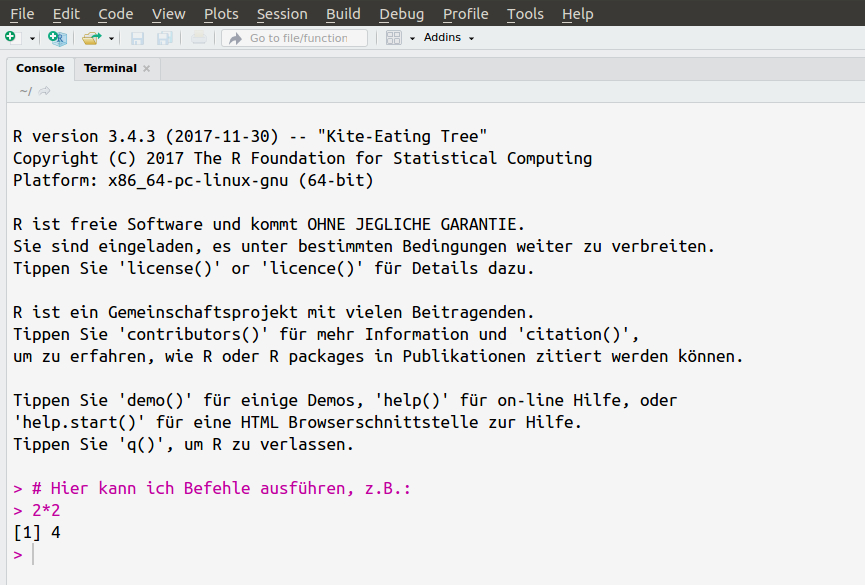
\includegraphics{../images/Konsole.jpg} So sieht die \texttt{R}-Konsole
in RStudio aus.
\end{marginfigure}

\begin{Shaded}
\begin{Highlighting}[]

\StringTok{"Hallo Welt!"}
\end{Highlighting}
\end{Shaded}

Wenn folgende Ausgabe erscheint, hat die Installation funktioniert:

\begin{verbatim}
[1] "Hallo Welt!"
\end{verbatim}

\section{\texorpdfstring{Die
\texttt{R}-Konsole}{Die R-Konsole}}\label{die-r-konsole}

Befehle können wir in \texttt{R} in die Konsole eingeben. Wir können das
als Kommunikation verstehen: Wir teilen \texttt{R} etwas mit, und
\texttt{R} gibt uns dazu passend etwas zurück -- \textbf{wenn unsere
Anfrage ein \emph{syntaktisch} korrekter \texttt{R}-Befehl war}.
Andernfalls gibt uns \texttt{R} eine Fehlermeldung zurück. Zum Beispiel
können wir die \texttt{R}-Konsole als Taschenrechner benutzen:

\begin{Shaded}
\begin{Highlighting}[]
\DecValTok{1} \OperatorTok{+}\StringTok{ }\DecValTok{3}
\end{Highlighting}
\end{Shaded}

\begin{verbatim}
[1] 4
\end{verbatim}

\begin{Shaded}
\begin{Highlighting}[]
\DecValTok{3} \OperatorTok{-}\StringTok{ }\DecValTok{17}
\end{Highlighting}
\end{Shaded}

\begin{verbatim}
[1] -14
\end{verbatim}

\begin{Shaded}
\begin{Highlighting}[]
\DecValTok{3} \OperatorTok{*}\StringTok{ }\DecValTok{2}
\end{Highlighting}
\end{Shaded}

\begin{verbatim}
[1] 6
\end{verbatim}

\begin{Shaded}
\begin{Highlighting}[]
\DecValTok{3}\OperatorTok{^}\DecValTok{2}
\end{Highlighting}
\end{Shaded}

\begin{verbatim}
[1] 9
\end{verbatim}

\begin{Shaded}
\begin{Highlighting}[]
\DecValTok{3}\OperatorTok{^}\DecValTok{2} \OperatorTok{+}\StringTok{ }\DecValTok{4}\OperatorTok{^}\DecValTok{2}
\end{Highlighting}
\end{Shaded}

\begin{verbatim}
[1] 25
\end{verbatim}

\begin{Shaded}
\begin{Highlighting}[]
\DecValTok{10}\OperatorTok{/}\DecValTok{5}
\end{Highlighting}
\end{Shaded}

\begin{verbatim}
[1] 2
\end{verbatim}

\begin{Shaded}
\begin{Highlighting}[]
\NormalTok{## Auf Klammerung achten:}
\NormalTok{(}\DecValTok{3} \OperatorTok{+}\StringTok{ }\DecValTok{5}\NormalTok{)}\OperatorTok{/}\DecValTok{2}
\end{Highlighting}
\end{Shaded}

\begin{verbatim}
[1] 4
\end{verbatim}

\begin{Shaded}
\begin{Highlighting}[]
\DecValTok{3} \OperatorTok{+}\StringTok{ }\DecValTok{5}\OperatorTok{/}\DecValTok{2}
\end{Highlighting}
\end{Shaded}

\begin{verbatim}
[1] 5.5
\end{verbatim}

\section{Der Skript-Editor}\label{der-skript-editor}

Zumeist werden wir \texttt{R}-Code nicht nur in der Konsole schreiben
und ausführen. Wenn wir einen Befehl in der Konsole geschrieben und mit
\texttt{Enter} ausgeführt haben, ist er ja quasi verschwunden.\footnote{Praktisch:
  Wenn ich mich in der Konsole befinde, kann ich mit den Pfeil-Tasten
  (vor allem wichtig: Pfeil-nach-oben) auf meine letzten Befehle wieder
  zugreifen. Probiert es aus.} Um Analysen übersichtlich,
nachvollziehbar und reproduzierbar zu gestalten, speichern wir unseren
Code in sogenannten Quellcode-Dateien ab. Dafür gibt es in RStudio (und
auch in anderen \texttt{R}-Umgebungen) einen Texteditor. Wir können eine
neue Quellcode-Datei unter ``Datei \(\to\) Neue Datei \(\to\) R Skript''
öffnen. Darin können wir unseren R-Code schreiben und permanent auf
unserem Computer abspeichern (und ggf. mit anderen Personen teilen).
Textdateien, die R-Code enthalten, speichern wir mit der Dateiendung
``.r'' oder ``.R'' ab.

Das Praktische: Wenn wir Code im Editor schreiben, können wir ihn auch
direkt von dort ausführen; wir müssen ihn nicht noch einmal in die
Konsole ``copy-pasten''. Das funktioniert so: Wenn sich mein Cursor in
einer Zeile befindet und ich \texttt{STRG-Enter} drücke, wird der Code
in dieser Zeile ausgeführt. Wenn ich einen Code-Abschnitt markiere, kann
ich ebenso mit \texttt{STRG-Enter} genau diesen Abschnitt ausführen. Der
Code wird in diesen Fällen an die Konsole gesendet, die dann die
Ausführung des Codes für uns übernimmt.

\section{Kommentare}\label{kommentare}

Wenn ein \texttt{\#}-Symbol in die Konsole oder den Skript-Editor
geschrieben wird, wird der Rest dessen, was in dieser Zeile steht, nicht
mehr interpretiert, d.h.: nicht als R-Code ausgeführt. Beispiel:

\begin{Shaded}
\begin{Highlighting}[]

\CommentTok{# 5 + 5 }
\CommentTok{# nichts ist passiert - `R` gibt mir nicht 10 aus}
\end{Highlighting}
\end{Shaded}

Man nutzt \texttt{\#}, um Code zu ``kommentieren'', das heißt um zu
erklären und zu dokumentieren, was der geschriebene Code macht. Diese
Kommentare fügt man in den Quelldateien ein, in denen man die eigenen
Analysen abspeichert. Dieses Skript enthält viel
\texttt{R}-Code,\footnote{Codeblöcke im Skript bestehen immer aus dem
  eigentlichen Code (dieser ist leicht grau hinterlegt) und der
  \emph{Ausgabe}, die bei Eingabe des Codes auch so in der
  \texttt{R}-Konsole erscheinen würde. Den Code könnt ihr auch selbst
  per \emph{Copy-\&-Paste} nachvollziehen (was ich auch empfehle). Die
  Ausgabe des Codes erkennt ihr meistens daran, dass sie mit
  \texttt{{[}1{]}} startet; so wird in der \texttt{R}-Konsole das erste
  Element der Ausgabe eines Vektors gekennzeichnet (siehe Kapitel 2).}
den ich stets kommentiere. (Ich habe die Angewohnheit, ein doppeltes
\texttt{\#\#} am Anfang einer Zeile zu benutzen, aber das hat keinerlei
Bedeutung.) Gewöhnt euch ebenfalls an, \textbf{immer} euren eigenen Code
zu kommentieren. Das gilt sowohl für ``richtige'' Projekte als auch für
Übungsaufgaben. Das Kommentieren für Code ist vor allem nützlich, um
anderen Personen euren Code zugänglich und verständlich zu machen. Im
häufigsten Fall seid ihr selbst in zwei Wochen diese ``andere'' Person.

\section{Ausblick}\label{ausblick}

In den nächsten zwei Kapiteln beschäftigen wir uns zunächst damit, wie
\texttt{R} Daten darstellt. Dabei betrachten wir zunächst die
grundlegenste Datenstruktur, den Vektor
(\protect\hyperlink{vektoren}{Kapitel 2}). Danach lernen wir
\texttt{data.frames} kennen (\protect\hyperlink{dataframes}{Kapitel 3}),
die in \texttt{R} Datentabellen darstellen, wie wir sie auch aus Excel
oder SPSS kennen. In \protect\hyperlink{psychometrie}{Kapitel 4} werden
wir psychometrische Datenauswertungen durchführen und dabei das Wissen
anwenden, das wir zuvor erworben haben.

\hypertarget{vektoren}{\chapter{Vektoren}\label{vektoren}}

Die einfachste und wichtigste Datenstruktur von \texttt{R} ist der
\emph{Vektor}. Ein Vektor ist beispielsweise eine einzelne Zahl wie in
den Taschenrechner-Berechnungen oben. So gilt für die Berechnung
\texttt{1\ +\ 3}:

\begin{itemize}
\tightlist
\item
  \texttt{1} ist ein Vektor
\item
  \texttt{3} ein Vektor
\item
  das Ergebnis \texttt{4} ist auch ein Vektor
\end{itemize}

Das Interessante an Vektoren ist, dass der ein-elementige Vektor nur ein
Spezialfall ist. Im Normalfall können Vektoren mehrere Elemente
enthalten; die ``atomare'' Einheit in \texttt{R} ist also nicht ein
einzelnes Element, sondern gleich eine Aneinanderreihung beliebig vieler
gleichartiger Elemente, etwa Zahlen.\footnote{Interessanterweise gibt es
  sogar Vektoren der Länge 0 -- also Vektoren, die gar kein Element
  beinhalten. Das soll uns aber erst einmal nicht beschäftigen.}
Statistische Berechnungen -- wie die Berechnung eines Mittelwerts oder
einer Standardabweichung -- lassen sich direkt auf einer Menge an Daten
durchführen, da diese in \textbf{einem} Vektor gespeichert sind. Diese
``Vektorbasiertheit'' ist vermutlich die größte Stärke von \texttt{R}
für statistische Berechnungen.

Elemente zu Vektoren zusammenfügen (sprich: \textbf{mehrere} Vektoren zu
\textbf{einem} Vektor zusammenfügen) funktioniert mit der
\emph{Funktion} \texttt{c} -- die vermutlich basalste Funktion in
\texttt{R}. Sie ist so simpel und grundlegend, dass man sie
gegebenenfalls vergisst, wenn man sie braucht -- versucht, sie zu
erinnern!

\begin{Shaded}
\begin{Highlighting}[]
\NormalTok{## Füge mehrere Zahlen zu einem Vektor}
\NormalTok{## zusammen:}
\KeywordTok{c}\NormalTok{(}\FloatTok{0.5}\NormalTok{, }\DecValTok{1}\NormalTok{, }\FloatTok{1.5}\NormalTok{)  }\CommentTok{# Kommazahlen mit DezimalPUNKT schreiben}
\end{Highlighting}
\end{Shaded}

\begin{verbatim}
[1] 0.5 1.0 1.5
\end{verbatim}

Man kann die Funktion \texttt{c} auch auf eine einzelne Zahl anwenden.
Das ist dasselbe als würde man nur die Zahl eingeben:

\begin{Shaded}
\begin{Highlighting}[]
\KeywordTok{c}\NormalTok{(}\DecValTok{1}\NormalTok{)}
\end{Highlighting}
\end{Shaded}

\begin{verbatim}
[1] 1
\end{verbatim}

Folgendes geht auch, da \texttt{c} mehrere Vektoren zu \textbf{einem
einzelnen} Vektor ``verschmilzt'':

\begin{Shaded}
\begin{Highlighting}[]
\KeywordTok{c}\NormalTok{(}\FloatTok{0.5}\NormalTok{, }\DecValTok{1}\NormalTok{, }\FloatTok{1.5}\NormalTok{, }\KeywordTok{c}\NormalTok{(}\DecValTok{1}\NormalTok{, }\DecValTok{2}\NormalTok{, }\DecValTok{3}\NormalTok{))}
\end{Highlighting}
\end{Shaded}

\begin{verbatim}
[1] 0.5 1.0 1.5 1.0 2.0 3.0
\end{verbatim}

Auf mehrelementigen Vektoren kann man statistische Berechnungen
durchführen, wie etwa die Bestimmung des arithmetischen Mittels, einer
Standardabweichung, der Varianz, oder des Minimums oder
Maximums:\footnote{\texttt{R} würde oft auch bei einelementigen Vektoren
  ein Ergebnis ausgeben, aber das ist zum Beispiel beim Mittelwert wenig
  sinnvoll.}

\begin{Shaded}
\begin{Highlighting}[]
\NormalTok{## Berechne einen Mittelwert}
\KeywordTok{mean}\NormalTok{(}\KeywordTok{c}\NormalTok{(}\FloatTok{0.5}\NormalTok{, }\DecValTok{1}\NormalTok{, }\FloatTok{1.5}\NormalTok{))}
\end{Highlighting}
\end{Shaded}

\begin{verbatim}
[1] 1
\end{verbatim}

\begin{Shaded}
\begin{Highlighting}[]
\NormalTok{## Berechne eine Standardabweichung}
\KeywordTok{sd}\NormalTok{(}\KeywordTok{c}\NormalTok{(}\FloatTok{0.5}\NormalTok{, }\DecValTok{1}\NormalTok{, }\FloatTok{1.5}\NormalTok{))}
\end{Highlighting}
\end{Shaded}

\begin{verbatim}
[1] 0.5
\end{verbatim}

\begin{Shaded}
\begin{Highlighting}[]
\NormalTok{## Berechne eine Varianz:}
\KeywordTok{var}\NormalTok{(}\KeywordTok{c}\NormalTok{(}\FloatTok{0.5}\NormalTok{, }\DecValTok{1}\NormalTok{, }\FloatTok{1.5}\NormalTok{))}
\end{Highlighting}
\end{Shaded}

\begin{verbatim}
[1] 0.25
\end{verbatim}

\begin{Shaded}
\begin{Highlighting}[]
\NormalTok{## Und jetzt noch einmal die}
\NormalTok{## Standardabweichung:}
\KeywordTok{sqrt}\NormalTok{(}\KeywordTok{var}\NormalTok{(}\KeywordTok{c}\NormalTok{(}\FloatTok{0.5}\NormalTok{, }\DecValTok{1}\NormalTok{, }\FloatTok{1.5}\NormalTok{)))  }\CommentTok{# was ist `sqrt`?}
\end{Highlighting}
\end{Shaded}

\begin{verbatim}
[1] 0.5
\end{verbatim}

\begin{Shaded}
\begin{Highlighting}[]
\NormalTok{## Minimum:}
\KeywordTok{min}\NormalTok{(}\KeywordTok{c}\NormalTok{(}\FloatTok{0.5}\NormalTok{, }\DecValTok{1}\NormalTok{, }\FloatTok{1.5}\NormalTok{))}
\end{Highlighting}
\end{Shaded}

\begin{verbatim}
[1] 0.5
\end{verbatim}

\begin{Shaded}
\begin{Highlighting}[]
\NormalTok{## Maximum:}
\KeywordTok{max}\NormalTok{(}\KeywordTok{c}\NormalTok{(}\FloatTok{0.5}\NormalTok{, }\DecValTok{1}\NormalTok{, }\FloatTok{1.5}\NormalTok{))}
\end{Highlighting}
\end{Shaded}

\begin{verbatim}
[1] 1.5
\end{verbatim}

In diesem Code-Block haben wir implizit einen wichtigen Bestandteil von
\texttt{R} kennengelernt: \emph{Funktionen}. Für den Einstieg reicht es
für uns, folgende Eigenschaften von Funktionen zu verstehen:

\begin{itemize}
\tightlist
\item
  Funktionen haben einen Namen -- etwa: \texttt{mean} oder \texttt{c}
\item
  Hinter dem Namen einer Funktion werden in Klammern ein oder mehrere
  \emph{Argumente} übergeben, etwa: ein Vektor
\item
  Wenn einer Funktion mehrere Argumente übergeben werden, werden diese
  mit Kommata separiert, etwa: \texttt{c(1,\ 2,\ 3)}\footnote{In den
    obigen Beispielen einfacher statistischer Berechnungen wird jeweils
    genau ein Argument übergeben, nämlich der Vektor, für den wir den
    Mittelwert, die Standardabweichung etc. berechnen wollten. Es ist
    auch möglich -- und auch üblich --, dass Funktionen mehrere
    Argumente annehmen, die ihr Verhalten bestimmen. Die Funktion
    \texttt{plot} etwa verfügt über eine kaum überschaubare Menge an
    möglichen Argumenten, die verwendet werden können, um das Aussehen
    einer Abbildung zu spezifizieren.}
\item
  Funktionen führen eine Berechnung durch und geben uns das Ergebnis
  zurück
\end{itemize}

Einfach gesagt nehmen also Funktionen Daten entgegen und geben wiederum
Daten zurück. Der Großteil unserer Arbeit mit \texttt{R} ist die
Anwendung von Funktionen. Es ist möglich Funktionsaufrufe zu
verschachteln, wie dieses Beispiel zeigte:

\begin{Shaded}
\begin{Highlighting}[]
\KeywordTok{sqrt}\NormalTok{(}\KeywordTok{var}\NormalTok{(}\KeywordTok{c}\NormalTok{(}\FloatTok{0.5}\NormalTok{, }\DecValTok{1}\NormalTok{, }\FloatTok{1.5}\NormalTok{)))}
\end{Highlighting}
\end{Shaded}

Hier wertet die Funktion \texttt{sqrt} (die Wurzel; engl. \emph{square
root}) das Ergebnis der Funktion \texttt{var} aus, um eine
Standardabweichnung zu bestimmen. Der Aufruf ist also äquivalent zu
\texttt{sqrt(0.25)}, da die Varianz von 0.5, 1, und 1.5 gleich 0.25 ist.
Diese Beobachtung offenbart eine weitere wichtige Eigenschaft von
\texttt{R}: Wir können unseren Code immer als das verstehen, was er
ergibt, wenn er von \texttt{R} ausgewertet wird. Es macht keinen
Unterschied, ob ich das Ergebnis einer Berechnung selber ``händisch''
aufschreibe -- also hier 0.25 --, oder Code schreibe, der mir dieses
Ergebnis generiert -- hier: \texttt{var(c(0.5,\ 1,\ 1.5))}.

~

Eine nützliche und oft verwendete Kurzform, um Vektoren aufsteigender,
ganzer Zahlen zu erstellen ist folgende:

\begin{Shaded}
\begin{Highlighting}[]
\DecValTok{1}\OperatorTok{:}\DecValTok{20}
\end{Highlighting}
\end{Shaded}

\begin{verbatim}
 [1]  1  2  3  4  5  6  7  8  9 10 11 12 13
[14] 14 15 16 17 18 19 20
\end{verbatim}

So lässt sich beispielsweise sehr einfach die Summe aller Zahlen von 1
bis 1,000 berechnen:

\begin{Shaded}
\begin{Highlighting}[]
\KeywordTok{sum}\NormalTok{(}\DecValTok{1}\OperatorTok{:}\DecValTok{1000}\NormalTok{)}
\end{Highlighting}
\end{Shaded}

\begin{verbatim}
[1] 500500
\end{verbatim}

Man kann auch absteigende Sequenzen erstellen:

\begin{Shaded}
\begin{Highlighting}[]
\DecValTok{5}\OperatorTok{:-}\DecValTok{5}
\end{Highlighting}
\end{Shaded}

\begin{verbatim}
 [1]  5  4  3  2  1  0 -1 -2 -3 -4 -5
\end{verbatim}

Diese Tabelle enthält einige nützliche Funktionen, die auf Vektoren
anwendbar sind (in \texttt{R}-Jargon: sie nehmen einen Vektor als
\emph{Argument} an) und jeweils selber auch einen Vektor zurückgeben:

\begin{longtable}[]{@{}ll@{}}
\toprule
Name & Funktionalität\tabularnewline
\midrule
\endhead
\texttt{mean} & Berechnet den Mittelwert eines Vektors\tabularnewline
\texttt{median} & Berechnet den Median eines Vektors\tabularnewline
\texttt{sum} & Berechnet die Summe aller Elemente eines
Vektors\tabularnewline
\texttt{max} & Gibt den größten Wert eines Vektors zurück\tabularnewline
\texttt{min} & Gibt den kleinsten Wert eines Vektors
zurück\tabularnewline
\texttt{length} & Gibt die Zahl der Elemente eines Vektors
zurück\tabularnewline
\texttt{sd} & Berechnet die Standardabweichung eines
Vektors\tabularnewline
\texttt{var} & Berechnet die Varianz eines Vektors\tabularnewline
\texttt{sort} & Sortiert einen Vektor aufsteigend\tabularnewline
\texttt{rev} & Kehrt die Reihenfolge der Elemente im Vektor
um\tabularnewline
\texttt{round} & Rundet die Elemente in einem Vektor\tabularnewline
\texttt{sqrt} & Berechnet für jedes Element im Vektor die
Quadratwurzel\tabularnewline
\texttt{unique} & Gibt alle unterschiedlichen Werte eines Vektors
aus\tabularnewline
\bottomrule
\end{longtable}

~

Für die Funktionen in dieser Tabelle gilt, dass sie zwar alle einen
Vektor zurückgeben, aber die Länge des Ausgabevektors unterschiedlich
sein kann. Die Funktionen \texttt{mean} und \texttt{sum} ergeben etwa
Vektoren der Länge 1, da sie genau einen Kennwert bestimmen. Die
Funktionen \texttt{sort}, \texttt{sqrt} und \texttt{round} geben
hingegen einen Vektor zurück, der aus genauso viele Elementen besteht
wie der Eingabevektor. Auch basale mathematische Berechnungen werden
gleich auf alle Elemente eines Vektors angewendet:

\begin{Shaded}
\begin{Highlighting}[]
\DecValTok{1}\OperatorTok{:}\DecValTok{10} \OperatorTok{*}\StringTok{ }\DecValTok{2}
\end{Highlighting}
\end{Shaded}

\begin{verbatim}
 [1]  2  4  6  8 10 12 14 16 18 20
\end{verbatim}

\begin{Shaded}
\begin{Highlighting}[]
\NormalTok{(}\DecValTok{1}\OperatorTok{:}\DecValTok{10} \OperatorTok{*}\StringTok{ }\DecValTok{2}\NormalTok{) }\OperatorTok{-}\StringTok{ }\DecValTok{1}
\end{Highlighting}
\end{Shaded}

\begin{verbatim}
 [1]  1  3  5  7  9 11 13 15 17 19
\end{verbatim}

Hierbei werden die Operationen \texttt{*\ 2} bzw. \texttt{-1} direkt auf
alle Elemente der Vektoren \texttt{1:10} bzw. \texttt{1:10\ *\ 2}
angewendet; die Ausgabe ist demnach jeweils ein Vektor der Länge 10. Bei
gleich langen Vektoren werden solche Operationen im Allgemeinen
\textbf{paarweise}\footnote{Ich werde dazu oft auch
  \emph{komponentenweise} sagen.} angewendet:

\begin{Shaded}
\begin{Highlighting}[]
\DecValTok{2}\OperatorTok{:}\DecValTok{4} \OperatorTok{*}\StringTok{ }\DecValTok{4}\OperatorTok{:}\DecValTok{6}  \CommentTok{# entspricht c(2*4, 3*5, 4*6)}
\end{Highlighting}
\end{Shaded}

\begin{verbatim}
[1]  8 15 24
\end{verbatim}

Dieses Verhalten ist typisch für \texttt{R}: Viele Funktionen und
Operationen in \texttt{R} arbeiten \textbf{komponentenweise}, wenn zwei
Vektoren gleicher Länge übergeben werden. Das Element an Position 1 im
einen Vektor wird dann mit dem Element an Position 1 im anderen Vektor
gepaart, das Element an Position 2 im einen Vektor mit dem Element an
Position 2 im anderen Vektor -- und so weiter.

Werden ein ein-elementiger Vektor und ein mehr-elementiger Vektor mit
einer Berechnung (etwa einer Addition) verknüpft, wird normalerweise das
einzelne Element mit allen Elementen des anderen Vektors
``gepaart''.\footnote{Wir werden nur diese Fälle betrachten: Entweder
  wird ein ein-elementiger Vektor mit einem längeren Vektor verknüpft
  oder zwei gleich lange Vektoren werden miteinander verknüpft. Es ist
  auch möglich, andere Kombinationen von Vektorlängen zu paaren, was wir
  jedoch erst einmal vernachlässigen (gebt bei Interesse einmal die
  Befehle \texttt{c(1,2)\ *\ 1:4} und \texttt{c(1,2)\ *\ 1:3} in die
  \texttt{R}-Konsole ein).}

\section{Variablen}\label{variablen}

Wir wollen unsere Daten nicht nur in der Konsole ausgeben lassen,
sondern auch abspeichern und damit arbeiten. Ein essentieller
Bestandteil einer jeden Programmiersprache ist es, Daten in Variablen
abzuspeichern. Variablen sind Namen, mit deren Hilfe wir auf
gespeicherte Daten zugreifen. Wenn wir Daten in einer Variablen
abgespeichert haben, können wir unter dem Namen der Variablen immer
wieder darauf zugreifen. In \texttt{R} funktioniert das mit der
Zuweisung ``\texttt{\textless{}-}'':

\begin{Shaded}
\begin{Highlighting}[]
\NormalTok{## Speichere einen Vektor in einer Variablen:}
\NormalTok{meinVektor <-}\StringTok{ }\KeywordTok{c}\NormalTok{(}\DecValTok{1}\NormalTok{, }\DecValTok{2}\NormalTok{, }\DecValTok{6}\NormalTok{, }\DecValTok{7}\NormalTok{, }\DecValTok{10}\NormalTok{)}
\end{Highlighting}
\end{Shaded}

Ich kann den Inhalt von Variablen in der \texttt{R}-Konsole ausgeben
lassen, wenn ich den Namen der Variablen in die Konsole schreibe und
\texttt{Enter} drücke:

\begin{Shaded}
\begin{Highlighting}[]
\NormalTok{meinVektor}
\end{Highlighting}
\end{Shaded}

\begin{verbatim}
[1]  1  2  6  7 10
\end{verbatim}

Ich kann Variablen in Berechnungen verwenden:

\begin{Shaded}
\begin{Highlighting}[]
\NormalTok{meinVektor }\OperatorTok{*}\StringTok{ }\DecValTok{2}
\end{Highlighting}
\end{Shaded}

\begin{verbatim}
[1]  2  4 12 14 20
\end{verbatim}

Ich kann Funktionen auf Variablen anwenden und das Ergebnis der Funktion
wiederum in einer Variablen speichern:

\begin{Shaded}
\begin{Highlighting}[]
\NormalTok{xx <-}\StringTok{ }\KeywordTok{mean}\NormalTok{(meinVektor)}

\NormalTok{## 'Zentrierter' numerischer Vektor:}
\NormalTok{meinVektor }\OperatorTok{-}\StringTok{ }\NormalTok{xx}
\end{Highlighting}
\end{Shaded}

\begin{verbatim}
[1] -4.2 -3.2  0.8  1.8  4.8
\end{verbatim}

Variablen können an jeder Stelle verwendet werden, an der man Daten
sonst ``händisch'' eingeben würde. Wir können jegliche Objekte -- nicht
nur Vektoren, sondern auch Datentabellen oder beliebig komplizierte
Ergebnisse von Berechnungen -- in Variablen speichern. Der Workflow in
\texttt{R} ist so ausgelegt, dass Zwischenergebnisse weiterverwendet
werden können. Hierbei unterscheidet es sich fundamental von SPSS, das
einen Unterschied zwischen Daten und ``Output'' macht. In \texttt{R}
kann das Ergebnis jeglicher Berechnung als Input einer anderen
Berechnung dienen.

~

\fbox{ \parbox{\textwidth}{

  \textbf{\\ Merke}
  
  In \texttt{R} kann (fast) alles in einer Variablen gespeichert und
  weiter verwendet werden.  } }

~

~

Wir können auch mit ``\texttt{=}'' Daten zu Variablen zuweisen. Das
funktioniert genauso wie ``\texttt{\textless{}-}'':

\begin{Shaded}
\begin{Highlighting}[]
\NormalTok{foo =}\StringTok{ }\DecValTok{1}\OperatorTok{:}\DecValTok{2}
\NormalTok{foo}
\end{Highlighting}
\end{Shaded}

\begin{verbatim}
[1] 1 2
\end{verbatim}

In \texttt{R} hat sich aus historischen Gründen die Konvention
durchgesetzt, \texttt{\textless{}-} zu verwenden, die ich in diesem
Skript auch befolgen werde. In vielen anderen Programmiersprachen werden
mit \texttt{=} Variablen zugewiesen.

\hypertarget{ausgabevsabspeichern}{\subsection{Ausgabe versus
Abspeichern}\label{ausgabevsabspeichern}}

Wir haben bereits zwei verschiedene Möglichkeiten gesehen,
Objekte\footnote{Bis jetzt kennen wir nur das Vektor-Objekt. In
  \texttt{R} gibt es aber ganz verschiedene ``Datencontainer'', die man
  allgemein als Objekte bezeichnet.} in \texttt{R} zu verwenden:

\begin{enumerate}
\def\labelenumi{\arabic{enumi}.}
\tightlist
\item
  Wir geben Objekte in der Konsole aus.
\item
  Wir speichern Objekte in einer Variable ab.
\end{enumerate}

Diese beiden Verwendungen sind \textbf{fundamental} unterschiedlich. Das
mag erst einmal trivial erscheinen, aber ist im Einzelfall nicht
unbedingt ersichtlich. Betrachten wir das folgende Beispiel:

\begin{Shaded}
\begin{Highlighting}[]
\NormalTok{bar <-}\StringTok{ }\KeywordTok{c}\NormalTok{(}\DecValTok{3}\NormalTok{, }\DecValTok{2}\NormalTok{, }\DecValTok{6}\NormalTok{, }\DecValTok{3}\NormalTok{, }\DecValTok{9}\NormalTok{, }\DecValTok{5}\NormalTok{, }\DecValTok{7}\NormalTok{, }\DecValTok{-3}\NormalTok{)}
\KeywordTok{sort}\NormalTok{(bar)}
\end{Highlighting}
\end{Shaded}

\begin{verbatim}
[1] -3  2  3  3  5  6  7  9
\end{verbatim}

Die Funktion \texttt{sort} sortiert den numerischen Vektor \texttt{bar}.
Wie sieht der Vektor \texttt{bar} nach der Operation aus? Es gibt zwei
Möglichkeiten:

\begin{enumerate}
\def\labelenumi{\arabic{enumi}.}
\tightlist
\item
  \texttt{bar} enthält den sortierten Vektor, den ich mithilfe von
  \texttt{sort(bar)} erstellt habe
\item
  \texttt{bar} enthält den unsortierten Vektor, den ich vor der
  Operation \texttt{sort(bar)} erstellt habe
\end{enumerate}

Wir können die Frage leicht klären, indem wir \texttt{bar} auf der
Konsole ausgeben:

\begin{Shaded}
\begin{Highlighting}[]
\NormalTok{bar}
\end{Highlighting}
\end{Shaded}

\begin{verbatim}
[1]  3  2  6  3  9  5  7 -3
\end{verbatim}

Offensichtlich hat \texttt{sort(bar)} den Vektor \texttt{bar} nicht
geändert. Das ist eine fundamentale Eigenschaft von \texttt{R}.
\textbf{Funktionen nehmen Daten an und sie geben Daten zurück -- sie
verändern aber nicht die eingegebenen Daten}. Wenn wir wollen, dass
\texttt{bar} die Zahlenfolge in sortierter Reihenfolge enthält, können
wir die folgende Befehlkette verwenden:

\begin{Shaded}
\begin{Highlighting}[]
\NormalTok{bar <-}\StringTok{ }\KeywordTok{c}\NormalTok{(}\DecValTok{3}\NormalTok{, }\DecValTok{2}\NormalTok{, }\DecValTok{6}\NormalTok{, }\DecValTok{3}\NormalTok{, }\DecValTok{9}\NormalTok{, }\DecValTok{5}\NormalTok{, }\DecValTok{7}\NormalTok{, }\DecValTok{-3}\NormalTok{)}
\NormalTok{bar <-}\StringTok{ }\KeywordTok{sort}\NormalTok{(bar)}
\end{Highlighting}
\end{Shaded}

In diesem Fall geht der Ursprungsvektor verloren und wir behalten nur
den sortieren Vektor. Generell gilt: wenn wir Daten in der Konsole
ausgeben lassen, verschwinden diese sozusagen im ``Nirvana''. Wenn wir
mit Daten weiterarbeiten wollen, müssen wir die Ausgabe einer Funktion
in einer Variablen speichern. Beide Verwendungszwecke sind denkbar:
Manchmal benötige ich nur die Ausgabe einer Berechnung, manchmal will
ich damit weiter rechnen.

\subsection{Variablennamen}\label{variablennamen}

Generell bestehen Variablennamen in \texttt{R} aus Buchstaben und Zahlen
und den Zeichen \texttt{.} und \texttt{\_}. Folgende Einschränkungen
sind zu beachten; wenn diese Anforderungen nicht berücksichtigt werden,
wird \texttt{R} eine Variablenzuweisung nicht akzeptieren.

\begin{itemize}
\tightlist
\item
  Variablennamen dürfen keine Leerzeichen enthalten

  \begin{itemize}
  \tightlist
  \item
    \texttt{bla\ bla\ \textless{}-\ c(1,\ 2)} funktioniert nicht
  \item
    \texttt{blabla\ \ \textless{}-\ c(1,\ 2)} funktioniert
  \end{itemize}
\item
  Variablennamen dürfen nicht mit einer Zahl starten

  \begin{itemize}
  \tightlist
  \item
    \texttt{1bla\ \textless{}-\ c(1,\ 2)} funktioniert nicht
  \item
    \texttt{bla1\ \textless{}-\ c(1,\ 2)} funktioniert
  \end{itemize}
\item
  Variablennamen dürfen keine Sonderzeichen außer \texttt{\_} oder
  \texttt{.} enthalten

  \begin{itemize}
  \tightlist
  \item
    \texttt{bla-bla\ \textless{}-\ c(1,\ 2)} funktioniert nicht
  \item
    \texttt{bla\%bla\ \textless{}-\ c(1,\ 2)} funktioniert nicht
  \item
    \texttt{bla\_bla\ \textless{}-\ c(1,\ 2)} funktioniert
  \item
    \texttt{bla.bla\ \textless{}-\ c(1,\ 2)} funktioniert
  \end{itemize}
\item
  Groß- / Kleinschreibung ist relevant (man sagt, dass Variablennamen in
  \texttt{R} ``case-sensitive'' sind)

  \begin{itemize}
  \tightlist
  \item
    ``\texttt{bla\ \textless{}-\ 1}'' ist nicht das Gleiche wie
    ``\texttt{Bla\ \textless{}-\ 1}'' oder gar
    ``\texttt{BLA\ \textless{}-\ 1}''
  \end{itemize}
\end{itemize}

Eine fundamentale Schwierigkeit beim Programmieren ist das Finden
\emph{guter} Variablennamen. \texttt{bla} und \texttt{blabla} sind
denkbar schlechte Variablennamen. Gute Variablennamen \emph{sprechen},
d.h. sie machen eine Aussage darüber, was für Daten sie beinhalten.

\begin{Shaded}
\begin{Highlighting}[]
\NormalTok{## Schlechter Variablenname:}
\NormalTok{foo <-}\StringTok{ }\KeywordTok{mean}\NormalTok{(age)}

\NormalTok{## Ggf. etwas besser:}
\NormalTok{mean_age <-}\StringTok{ }\KeywordTok{mean}\NormalTok{(age)}
\end{Highlighting}
\end{Shaded}

Beachtet \textbf{immer} folgende Regel: Variablennamen sollten nicht
lügen, also verwendet niemals einen Namen der folgenden Art:

\begin{Shaded}
\begin{Highlighting}[]
\NormalTok{mean_age <-}\StringTok{ }\KeywordTok{sd}\NormalTok{(age) }\CommentTok{# Niemals machen!}
\end{Highlighting}
\end{Shaded}

Man ist schnell geneigt einen unsinnigen Variablennamen zu vergeben, um
keine Zeit mit der Namensfindung zu verschwenden -- man hat ja
schließlich wichtigen Code zu schreiben! Man sollte sich jedoch so gut
wie immer kurz Zeit nehmen, einen sinnigen Namen zu finden -- das
zukünftige Selbst wird es einem danken. Unsinnige Variablennamen sind in
Ordnung, wenn man sich zu 100\% sicher ist, dass man die Variable nach
einmaliger Nutzung nicht mehr verwendet. Wenn man eine Variable nicht
mehr benutzen möchte, kann man sie mit der \texttt{rm} Funktion löschen:

\begin{Shaded}
\begin{Highlighting}[]
\NormalTok{foo <-}\StringTok{ }\DecValTok{1}\OperatorTok{:}\DecValTok{10} \CommentTok{# Wegwerfvariable}
\KeywordTok{rm}\NormalTok{(foo)}
\NormalTok{foo}
\NormalTok{Fehler}\OperatorTok{:}\StringTok{ }\NormalTok{Objekt }\StringTok{'foo'}\NormalTok{ nicht gefunden}
\end{Highlighting}
\end{Shaded}

Weiterhin ist es guter Stil \emph{konsistent} in der Vergebung der
Variablennamen zu sein. Variablennamen sollen einen semantischen Gehalt
haben, das heißt sie machen eine Aussage darüber, welche Daten sie
enthalten. Häufig ist diese Information nicht in einem Wort erklärbar.
Um auszusagen, dass eine Variable ``das mittlere Alter'' enthält, müssen
mindestens die Anteile ``mittel'' und ``Alter'' enthalten sein. Wie soll
das verknüpft werden? Verschiedene Konventionen existieren; wichtig ist,
dass ihr euch konsistent für eine Variante entscheidet.\footnote{Ich
  werde von dieser Regel in diesem Skript abweichen.}

\begin{Shaded}
\begin{Highlighting}[]
\NormalTok{## Mögliche Konventionen der Namensgebung von Variablen:}
\NormalTok{mean_age <-}\StringTok{ }\KeywordTok{mean}\NormalTok{(age)}
\NormalTok{mean.age <-}\StringTok{ }\KeywordTok{mean}\NormalTok{(age)}
\NormalTok{meanAge  <-}\StringTok{ }\KeywordTok{mean}\NormalTok{(age)}

\NormalTok{## keine gute Konvention:}
\NormalTok{meanage  <-}\StringTok{ }\KeywordTok{mean}\NormalTok{(age)}
\end{Highlighting}
\end{Shaded}

\section{Datentypen von Vektoren}\label{datentypen-von-vektoren}

In \texttt{R} hat jeder Vektor einen Datentyp. Bis jetzt haben wir nur
mit Zahlen gearbeitet. Dieser Datentyp heißt in \texttt{R} ``numeric''.
Der Datentyp eines Vektors bestimmt, was für Operationen wir damit
durchführen können. Vektoren vom Typ ``numeric'' etwa kann man addieren,
multiplizieren und so weiter. Es gibt weitere Datentypen, die wir
benutzen, um unterschiedliche Informationen darzustellen.

\subsection{\texorpdfstring{\texttt{character}}{character}}\label{character}

\texttt{character} ist der Datentyp, der Text kennzeichnet. Text wird
mit doppelten oder einfachen Anführungszeichen angegeben:

\begin{Shaded}
\begin{Highlighting}[]
\StringTok{"Hallo Welt!"}
\end{Highlighting}
\end{Shaded}

\begin{verbatim}
[1] "Hallo Welt!"
\end{verbatim}

\begin{Shaded}
\begin{Highlighting}[]

\NormalTok{mein_text <-}\StringTok{ 'bla bla bla'}

\NormalTok{## zwei-elementiger Vektor vom Typ character:}
\NormalTok{mein_text2 <-}\StringTok{ }\KeywordTok{c}\NormalTok{(}\StringTok{"Cronbachs"}\NormalTok{, }\StringTok{"Alpha"}\NormalTok{)}
\end{Highlighting}
\end{Shaded}

Mit Texten können wir andere Operationen durchführen als mit Zahlen,
etwa ergibt Folgendes eine Fehlermeldung\footnote{Leider sind
  Fehlermeldungen in \texttt{R} oftmals sehr kryptisch und gerade für
  Anfänger schwer verständlich.} und ergibt auch gar keinen Sinn, da man
Text nicht mit einer Zahl multiplizieren kann:

\begin{Shaded}
\begin{Highlighting}[]
\StringTok{"bla"} \OperatorTok{*}\StringTok{ }\DecValTok{2}
\NormalTok{Fehler }\ControlFlowTok{in} \StringTok{"bla"} \OperatorTok{*}\StringTok{ }\DecValTok{2} \OperatorTok{:}\StringTok{ }\NormalTok{nicht}\OperatorTok{-}\NormalTok{numerisches Argument}
\NormalTok{für binären Operator}
\end{Highlighting}
\end{Shaded}

In diesem Skript spielen Texte keine allzu große Rolle. Eine nützliche
Funktion, die Vektoren vom Typ \texttt{character} generiert, sei hier
jedoch kurz vorgestellt, da wir von ihr Gebrauch machen werden. Die
Funktion \texttt{paste0} kann verwendet werden, um mehrere Vektoren als
Text zusammenzufügen. Das wird nützlich sein, wenn wir in Datentabellen
auf bestimmte Spalten zugreifen wollen, denn dort gilt: Jedes Item steht
in einer Spalte. So lassen sich beispielsweise bequem 10
durchnummerierte Itemnamen als \texttt{character}-Vektor zusammenfügen:

\begin{Shaded}
\begin{Highlighting}[]
\NormalTok{items <-}\StringTok{ }\KeywordTok{paste0}\NormalTok{(}\StringTok{"item_"}\NormalTok{, }\DecValTok{1}\OperatorTok{:}\DecValTok{10}\NormalTok{)}
\end{Highlighting}
\end{Shaded}

Hierbei wird der Text ``item\_'' mit den Zahlen von 1 bis 10 gepaart.
Das Ergebnis ist ein 10-elementiger Vektor, wie wir auch so überprüfen
können:

\begin{Shaded}
\begin{Highlighting}[]
\KeywordTok{length}\NormalTok{(items)}
\end{Highlighting}
\end{Shaded}

\begin{verbatim}
[1] 10
\end{verbatim}

\begin{Shaded}
\begin{Highlighting}[]
\NormalTok{items}
\end{Highlighting}
\end{Shaded}

\begin{verbatim}
 [1] "item_1"  "item_2"  "item_3"  "item_4" 
 [5] "item_5"  "item_6"  "item_7"  "item_8" 
 [9] "item_9"  "item_10"
\end{verbatim}

Mit der Funktion \texttt{mode} können wir überprüfen, dass der Vektor
tatsächlich vom Typ \texttt{character} ist:\footnote{Die Ausgabe des
  Vektors macht uns auch schon eindeutig klar, dass es sich hier um
  einen Vektor vom Typ \texttt{character} handelt; die ausgegeben
  Elemente erscheinen nämlich in Anführungszeichen (``item\_1'',
  ``item\_2'', \ldots{})}

\begin{Shaded}
\begin{Highlighting}[]
\KeywordTok{mode}\NormalTok{(items)}
\end{Highlighting}
\end{Shaded}

\begin{verbatim}
[1] "character"
\end{verbatim}

Wenn man mit der Funktion \texttt{paste0} mehrere ein-elementige
Vektoren miteinander verknüpft, wird immer ein ein-elementiger Vektor
vom Typ \texttt{character} ausgegeben:

\begin{Shaded}
\begin{Highlighting}[]
\KeywordTok{paste0}\NormalTok{(}\StringTok{"item"}\NormalTok{, }\StringTok{"_"}\NormalTok{, }\DecValTok{1}\NormalTok{)  }\CommentTok{# nimmt beliebig viele Argumente an}
\end{Highlighting}
\end{Shaded}

\begin{verbatim}
[1] "item_1"
\end{verbatim}

Wie wir sehen werden, können wir in Datentabellen mit der Funktion
\texttt{paste0} Antworten auf gewünschte Items auswählen, da wir mit
Textvektoren auf die Namen von Tabellenspalten zugreifen können.

\subsection{\texorpdfstring{\texttt{logical}}{logical}}\label{logical}

Es hat sich als nützlich erwiesen, einen Datentyp einzuführen, der
``Wahrheit'' kodiert. Dieser Datentyp wird in \texttt{R} ``logical''
genannt; er kennt nur die Ausprägungen \texttt{TRUE} und \texttt{FALSE}.
Eine sonst gängige Bezeichnung für diesen Datentyp ist auch ``boolean''.

\begin{Shaded}
\begin{Highlighting}[]
\NormalTok{wahr <-}\StringTok{ }\OtherTok{TRUE}
\NormalTok{falsch <-}\StringTok{ }\OtherTok{FALSE}
\end{Highlighting}
\end{Shaded}

Wir werden häufig vom Typ \texttt{logical} Gebrauch machen, wenn wir in
Datentabellen Fälle auswählen (etwa alle weiblichen oder männlichen
Teilnehmer in einer Umfrage).

~

Mit logischen Werten kann man die logischen Operationen UND (in
\texttt{R}: \texttt{\&} ), ODER (in \texttt{R}: \texttt{\textbar{}} )
und NICHT (in \texttt{R}: \texttt{!} ) durchführen:\footnote{https://de.wikipedia.org/wiki/Boolesche\_Algebra\#
  Zweielementige\_boolesche\_Algebra}

\begin{Shaded}
\begin{Highlighting}[]
\NormalTok{## Logisches UND}
\OtherTok{TRUE} \OperatorTok{&}\StringTok{ }\OtherTok{TRUE}
\end{Highlighting}
\end{Shaded}

\begin{verbatim}
[1] TRUE
\end{verbatim}

\begin{Shaded}
\begin{Highlighting}[]
\OtherTok{TRUE} \OperatorTok{&}\StringTok{ }\OtherTok{FALSE}
\end{Highlighting}
\end{Shaded}

\begin{verbatim}
[1] FALSE
\end{verbatim}

\begin{Shaded}
\begin{Highlighting}[]
\OtherTok{FALSE} \OperatorTok{&}\StringTok{ }\OtherTok{FALSE}
\end{Highlighting}
\end{Shaded}

\begin{verbatim}
[1] FALSE
\end{verbatim}

\begin{Shaded}
\begin{Highlighting}[]
\NormalTok{## Logisches ODER}
\OtherTok{TRUE} \OperatorTok{|}\StringTok{ }\OtherTok{TRUE}
\end{Highlighting}
\end{Shaded}

\begin{verbatim}
[1] TRUE
\end{verbatim}

\begin{Shaded}
\begin{Highlighting}[]
\OtherTok{TRUE} \OperatorTok{|}\StringTok{ }\OtherTok{FALSE}
\end{Highlighting}
\end{Shaded}

\begin{verbatim}
[1] TRUE
\end{verbatim}

\begin{Shaded}
\begin{Highlighting}[]
\OtherTok{FALSE} \OperatorTok{|}\StringTok{ }\OtherTok{FALSE}
\end{Highlighting}
\end{Shaded}

\begin{verbatim}
[1] FALSE
\end{verbatim}

\begin{Shaded}
\begin{Highlighting}[]
\NormalTok{## Logisches NICHT}
\OperatorTok{!}\OtherTok{TRUE}
\end{Highlighting}
\end{Shaded}

\begin{verbatim}
[1] FALSE
\end{verbatim}

\begin{Shaded}
\begin{Highlighting}[]
\OperatorTok{!}\OtherTok{FALSE}
\end{Highlighting}
\end{Shaded}

\begin{verbatim}
[1] TRUE
\end{verbatim}

\textbf{Merke}: Auch diese logischen Operationen arbeiten
komponentenweise auf Vektoren, die mehr als ein Element enthalten:

\begin{Shaded}
\begin{Highlighting}[]
\KeywordTok{c}\NormalTok{(}\OtherTok{TRUE}\NormalTok{, }\OtherTok{FALSE}\NormalTok{, }\OtherTok{FALSE}\NormalTok{) }\OperatorTok{&}\StringTok{ }\KeywordTok{c}\NormalTok{(}\OtherTok{TRUE}\NormalTok{, }\OtherTok{TRUE}\NormalTok{, }\OtherTok{FALSE}\NormalTok{)}
\end{Highlighting}
\end{Shaded}

\begin{verbatim}
[1]  TRUE FALSE FALSE
\end{verbatim}

\begin{Shaded}
\begin{Highlighting}[]
\KeywordTok{c}\NormalTok{(}\OtherTok{TRUE}\NormalTok{, }\OtherTok{FALSE}\NormalTok{, }\OtherTok{FALSE}\NormalTok{) }\OperatorTok{|}\StringTok{ }\KeywordTok{c}\NormalTok{(}\OtherTok{TRUE}\NormalTok{, }\OtherTok{TRUE}\NormalTok{, }\OtherTok{FALSE}\NormalTok{)}
\end{Highlighting}
\end{Shaded}

\begin{verbatim}
[1]  TRUE  TRUE FALSE
\end{verbatim}

\subsection{\texorpdfstring{\texttt{factor}}{factor}}\label{factor}

\texttt{factor} Vektoren stellen kategoriale Variablen dar -- etwa die
unabhängigen Variablen in einer ANOVA. So können wir einen Vektor vom
Typ \texttt{factor} erstellen:

\begin{Shaded}
\begin{Highlighting}[]
\NormalTok{laune <-}\StringTok{ }\KeywordTok{c}\NormalTok{(}\DecValTok{1}\NormalTok{, }\DecValTok{2}\NormalTok{, }\DecValTok{3}\NormalTok{, }\DecValTok{1}\NormalTok{, }\DecValTok{2}\NormalTok{, }\DecValTok{1}\NormalTok{)}

\NormalTok{laune_faktor <-}\StringTok{ }\KeywordTok{factor}\NormalTok{(laune, }\DataTypeTok{levels =} \KeywordTok{c}\NormalTok{(}\DecValTok{1}\NormalTok{, }\DecValTok{2}\NormalTok{, }
    \DecValTok{3}\NormalTok{), }\DataTypeTok{labels =} \KeywordTok{c}\NormalTok{(}\StringTok{":("}\NormalTok{, }\StringTok{":)"}\NormalTok{, }\StringTok{":D"}\NormalTok{))}
\NormalTok{laune_faktor}
\end{Highlighting}
\end{Shaded}

\begin{verbatim}
[1] :( :) :D :( :) :(
Levels: :( :) :D
\end{verbatim}

Die Funktion \texttt{factor} kann genutzt werden, um numerische Werte in
\texttt{factor} umzuwandeln. Dabei kann man die \texttt{levels}
spezifizieren, d.h. die Werte, die der Vektor annimmt, \textbf{bevor} er
in \texttt{factor} umgewandelt wird -- hier \texttt{1}, \texttt{2} und
\texttt{3}. \texttt{labels} wird verwendet, um anzugeben, wie die
Faktorstufen angezeigt werden sollen. Das ist ähnlich den Wertelabels,
die man in SPSS vergeben kann. Der Unterschied in \texttt{R}: Wenn ich
eine Variable in \texttt{factor} umwandle, kann ich damit keine
numerischen Berechnungen mehr durchführen. Für \texttt{laune\_faktor}
kann ich keinen Mittelwert mehr berechnen, da Vektoren vom Typ
\texttt{factor} kategoriale Variablen darstellen:

\begin{Shaded}
\begin{Highlighting}[]
\KeywordTok{mean}\NormalTok{(laune)}
\end{Highlighting}
\end{Shaded}

\begin{verbatim}
[1] 1.666667
\end{verbatim}

\begin{Shaded}
\begin{Highlighting}[]
\KeywordTok{mean}\NormalTok{(laune_faktor)}
\end{Highlighting}
\end{Shaded}

\begin{verbatim}
[1] NA
\end{verbatim}

Da die Berechnung nicht möglich ist, gibt \texttt{R} die folgende
``Warnmeldung'' aus:

\begin{Shaded}
\begin{Highlighting}[]

\NormalTok{Warnmeldung}\OperatorTok{:}
\NormalTok{In }\KeywordTok{mean.default}\NormalTok{(laune_faktor) }\OperatorTok{:}
\StringTok{  }\NormalTok{argument is not numeric or logical}\OperatorTok{:}\StringTok{ }\NormalTok{returning }\OtherTok{NA}
\end{Highlighting}
\end{Shaded}

\subsection{\texorpdfstring{\texttt{NA}}{NA}}\label{na}

\texttt{R} hat einen eigenen Datentyp, um fehlende Werte zu kodieren:
\texttt{NA}.\footnote{Eigentlich ist \texttt{NA} kein eigener Datentyp.
  In \texttt{R} hat jeder Vektor \textbf{nur genau einen} Datentyp. Es
  ist beispielsweise nicht möglich, dass in einem Vektor gleichzeitig
  Werte vom Typ \texttt{numeric}, \texttt{character} und \texttt{factor}
  vorkommen. \texttt{NA}-Werte können jedoch in Kombination mit jedem
  Datentyp vorkommen. Sie kodieren dann die Abwesenheit eines Datums;
  dieses Datum hätte -- wenn es nicht fehlen würde -- den Datentyp des
  Vektors.} Da wir mit echten Datensätzen arbeiten, die oftmals
``messy'' sind, d.h. nicht notwendigerweise vollständig, ist diese
Eigenschaft sehr nützlich. Gerade bei der Arbeit mit Daten in der
psychologischen Diagnostik ist dies wichtig: Menschen geben in
Fragebögen eben nicht immer auf alle Fragen eine Antwort.

Man kann selber Vektoren erstellen, die fehlende Werte enthalten:

\begin{Shaded}
\begin{Highlighting}[]
\NormalTok{messy_data <-}\StringTok{ }\KeywordTok{c}\NormalTok{(}\DecValTok{1}\NormalTok{, }\DecValTok{3}\NormalTok{, }\DecValTok{2}\NormalTok{, }\DecValTok{9}\NormalTok{, }\DecValTok{3}\NormalTok{, }\OtherTok{NA}\NormalTok{, }\DecValTok{6}\NormalTok{, }\OtherTok{NA}\NormalTok{, }\DecValTok{5}\NormalTok{)}
\end{Highlighting}
\end{Shaded}

Die Anwesenheit von fehlenden Werten hat Auswirkungen darauf, welche
Berechnungen \texttt{R} mit dem Vektor anstellen kann. Etwa können wir
nicht mehr ohne Weiteres einen Mittelwert berechnen:

\begin{Shaded}
\begin{Highlighting}[]
\KeywordTok{mean}\NormalTok{(messy_data)  }\CommentTok{# geht nicht wegen des fehlenden Werts}
\end{Highlighting}
\end{Shaded}

\begin{verbatim}
[1] NA
\end{verbatim}

Man muss \texttt{R} explizit mitteilen, dass man trotz des Auftretens
fehlender Werte einen Mittelwert ausrechnen möchte. Dies funktioniert
mit dem \emph{optionalen Argument} \texttt{na.rm}\footnote{Ein Argument
  heißt optional, wenn wir dafür keinen Wert angeben müssen. Stattdessen
  hat es einen sogenannten Standardwert, der angenommen wird, wenn wir
  das Argument nicht selber angeben. Der Standardwert des Arguments
  \texttt{na.rm} in der Funktion \texttt{mean} ist \texttt{FALSE}.} der
Funktion \texttt{mean}, welches wir auf \texttt{TRUE} setzen können. Mit
dem \emph{Argument} \texttt{na.rm} (``NA remove'') teilt man
\texttt{mean} mit, dass \texttt{NA} Werte bei der Berechnung des
Mittelwerts nicht berücksichtigt werden sollen (andere Funktionen wie
\texttt{sd} und \texttt{var} haben auch das Argument \texttt{na.rm}):

\begin{Shaded}
\begin{Highlighting}[]
\KeywordTok{mean}\NormalTok{(messy_data, }\DataTypeTok{na.rm =} \OtherTok{TRUE}\NormalTok{)}
\end{Highlighting}
\end{Shaded}

\begin{verbatim}
[1] 4.142857
\end{verbatim}

Hierbei nehmen wir zur Kenntnis, dass man Argumente von Funktionen
benennen kann -- was wir aber nicht immer machen. Dazu später mehr.

\section{Logische Vergleiche}\label{logische-vergleiche}

Wir können in \texttt{R} Eigenschaften von Vektoren mithilfe von
logischen Vergleichen erfragen. So kann man beispielsweise prüfen,
welche Werte eines numerischen Vektors (a) gleich, (b) größer (c)
kleiner, (d) größer gleich, (e) kleiner gleich oder (f) ungleich einem
bestimmten Wert sind. Diese Operationen sind fundamental für den
weiteren Verlauf des Seminars. Es wird sich gegebenenfalls lohnen, bei
den Themen Datenauswahl in Datentabellen noch einmal diesen Abschnitt zu
konsultieren (in Kapitel \protect\hyperlink{subset}{3}). Dieser
Code-Abschnitt stellt die grundlegenden logischen Vergleiche dar:

\begin{Shaded}
\begin{Highlighting}[]
\NormalTok{vergleichswert <-}\StringTok{ }\DecValTok{3}
\NormalTok{daten <-}\StringTok{ }\DecValTok{1}\OperatorTok{:}\DecValTok{5}
\NormalTok{daten }\OperatorTok{>}\StringTok{ }\NormalTok{vergleichswert}
\end{Highlighting}
\end{Shaded}

\begin{verbatim}
[1] FALSE FALSE FALSE  TRUE  TRUE
\end{verbatim}

\begin{Shaded}
\begin{Highlighting}[]
\NormalTok{daten }\OperatorTok{<}\StringTok{ }\NormalTok{vergleichswert}
\end{Highlighting}
\end{Shaded}

\begin{verbatim}
[1]  TRUE  TRUE FALSE FALSE FALSE
\end{verbatim}

\begin{Shaded}
\begin{Highlighting}[]
\NormalTok{daten }\OperatorTok{>=}\StringTok{ }\NormalTok{vergleichswert}
\end{Highlighting}
\end{Shaded}

\begin{verbatim}
[1] FALSE FALSE  TRUE  TRUE  TRUE
\end{verbatim}

\begin{Shaded}
\begin{Highlighting}[]
\NormalTok{daten }\OperatorTok{<=}\StringTok{ }\NormalTok{vergleichswert}
\end{Highlighting}
\end{Shaded}

\begin{verbatim}
[1]  TRUE  TRUE  TRUE FALSE FALSE
\end{verbatim}

\begin{Shaded}
\begin{Highlighting}[]
\NormalTok{daten }\OperatorTok{==}\StringTok{ }\NormalTok{vergleichswert}
\end{Highlighting}
\end{Shaded}

\begin{verbatim}
[1] FALSE FALSE  TRUE FALSE FALSE
\end{verbatim}

\begin{Shaded}
\begin{Highlighting}[]
\NormalTok{daten }\OperatorTok{!=}\StringTok{ }\NormalTok{vergleichswert}
\end{Highlighting}
\end{Shaded}

\begin{verbatim}
[1]  TRUE  TRUE FALSE  TRUE  TRUE
\end{verbatim}

Das Ergebnis dieser Operationen ist ein Vektor aus \texttt{TRUE} und
\texttt{FALSE} Werten. Die Werte nehmen \texttt{TRUE} an, wenn die
Zahlen die kleiner/größer/gleich Bedingung erfüllen -- andernfalls
\texttt{FALSE}. \textbf{Beachtet, dass auf Gleichheit mit dem
``doppelten'' \texttt{==} Operator getestet wird und nicht mit einem
einfachen \texttt{=}.} Dies ist eine häufige Quelle von Fehlern, die
schwierig zu entdecken sind. Betrachtet etwa folgenden Code -- was geht
hier schief?

\begin{Shaded}
\begin{Highlighting}[]
\NormalTok{daten =}\StringTok{ }\NormalTok{vergleichswert}
\end{Highlighting}
\end{Shaded}

Hierbei wird die Variable \texttt{daten} mit dem Wert in der Variablen
\texttt{vergleichswert} überschrieben, da \texttt{=} als Zuweisung
agiert:

\begin{Shaded}
\begin{Highlighting}[]
\NormalTok{daten}
\end{Highlighting}
\end{Shaded}

\begin{verbatim}
[1] 3
\end{verbatim}

Dies ist ein Beispiel für einen Fehler (\emph{Bug}), den man nicht
anhand von einer Fehlermeldung bemerkt, da der Befehl \emph{syntaktisch}
korrekt ist. Es ist jedoch problematisch, dass ich an dieser Stelle
meine Daten mit einem irrelevanten Wert überschrieben habe, und das bei
einem späteren Zugriff darauf vermutlich nicht beachten werde.

Welche logischen Vergleiche möglich sind, hängt vom Datentyp eines
Vektors ab. Für Vektoren vom typ \texttt{character} etwa macht eine
kleiner/größer Abfrage keinen Sinn, jedoch eine Abfrage auf
Gleichheit:\footnote{Für Vektoren vom Typ \texttt{factor} lässt sich auf
  dieselbe Art und Weise eine Abfrage auf Gleichheit umsetzen.}

\begin{Shaded}
\begin{Highlighting}[]
\NormalTok{text1 <-}\StringTok{ "Hallo Welt"}

\NormalTok{text1 }\OperatorTok{==}\StringTok{ "Hallo Welt"}
\end{Highlighting}
\end{Shaded}

\begin{verbatim}
[1] TRUE
\end{verbatim}

\begin{Shaded}
\begin{Highlighting}[]
\NormalTok{text1 }\OperatorTok{==}\StringTok{ "Hallo Welt!"}
\end{Highlighting}
\end{Shaded}

\begin{verbatim}
[1] FALSE
\end{verbatim}

Wenn zwei Vektoren gleicher Länge mit logischen Operatoren verglichen
werden, werden die Elemente komponentenweise verglichen:

\begin{Shaded}
\begin{Highlighting}[]
\NormalTok{score_test1 <-}\StringTok{ }\KeywordTok{c}\NormalTok{(}\DecValTok{23}\NormalTok{, }\DecValTok{19}\NormalTok{, }\DecValTok{44}\NormalTok{, }\DecValTok{18}\NormalTok{, }\DecValTok{25}\NormalTok{, }\DecValTok{22}\NormalTok{)}
\NormalTok{score_test2 <-}\StringTok{ }\KeywordTok{c}\NormalTok{(}\DecValTok{26}\NormalTok{, }\DecValTok{23}\NormalTok{, }\DecValTok{29}\NormalTok{, }\DecValTok{18}\NormalTok{, }\DecValTok{32}\NormalTok{, }\DecValTok{19}\NormalTok{)}

\NormalTok{score_test1 }\OperatorTok{>}\StringTok{ }\NormalTok{score_test2}
\end{Highlighting}
\end{Shaded}

\begin{verbatim}
[1] FALSE FALSE  TRUE FALSE FALSE  TRUE
\end{verbatim}

\begin{Shaded}
\begin{Highlighting}[]
\NormalTok{score_test1 }\OperatorTok{==}\StringTok{ }\NormalTok{score_test2}
\end{Highlighting}
\end{Shaded}

\begin{verbatim}
[1] FALSE FALSE FALSE  TRUE FALSE FALSE
\end{verbatim}

\textbf{Anwendungsbeispiel: Überprüfe das Gesetz der großen Zahlen}

~

Häufig verwendet man die Vergleichsoperatoren, um zu prüfen, wie viele
Daten eine bestimmte Eigenschaft erfüllen. Dafür verknüpfen wir die
Vergleichsoperatoren mit den Funktionen \texttt{sum} oder \texttt{mean}.

Dafür bietet sich ein Beispiel aus der Statistik an: Wie viele von 1,000
Zufallsdaten aus einer Standardnormalverteilung sind größer als 1?
\texttt{R} hat zahlreiche Funktionen, um Zufallszahlen aus verschiedenen
Verteilungen zu ``samplen''. Mit \texttt{rnorm} lassen sich
Zufallszahlen generieren, die einer Normalverteilungen folgen; wenn man
keine weiteren Argumente angibt, ist die Standardnormalverteilung
gemeint, die einen Mittelwert von \texttt{0} und eine Standardabweichung
von \texttt{1} hat:

\begin{Shaded}
\begin{Highlighting}[]
\NormalTok{## Erstelle 1,000 Zufallsdaten:}
\NormalTok{zufallsdaten <-}\StringTok{ }\KeywordTok{rnorm}\NormalTok{(}\DecValTok{1000}\NormalTok{)}
\end{Highlighting}
\end{Shaded}

Zur Verdeutlichung: Der Vektor \texttt{zufallsdaten} enthält jetzt 1,000
Elemente, wie wir mit der Funktion \texttt{length} leicht überprüfen
können:

\begin{Shaded}
\begin{Highlighting}[]
\KeywordTok{length}\NormalTok{(zufallsdaten)}
\end{Highlighting}
\end{Shaded}

\begin{verbatim}
[1] 1000
\end{verbatim}

Die Funktion \texttt{head} zeigt uns die ersten sechs Werte des Vektors
an. \texttt{head} ist sehr praktisch, um sich schnell einen Blick über
Daten zu verschaffen. Das machen wir hier auch, da wir nicht alle 1,000
Werte in die Konsole schreiben wollen:

\begin{Shaded}
\begin{Highlighting}[]
\KeywordTok{head}\NormalTok{(zufallsdaten)}
\end{Highlighting}
\end{Shaded}

\begin{verbatim}
[1]  0.6663414  0.4002734  1.0811086
[4]  0.3137942  0.8305779 -0.4346536
\end{verbatim}

Wir können die Daten mithilfe eines Histogramms betrachten, um uns davon
zu überzeugen, dass sie tatsächlich normalverteilt sind -- sich also der
Großteil der Daten um die \texttt{0} tummelt und extreme Werte in beide
Richtungen seltener werden (dieser Code muss nicht verstanden werden):

\begin{Shaded}
\begin{Highlighting}[]
\NormalTok{## Male Histogram}
\KeywordTok{hist}\NormalTok{(zufallsdaten, }\DataTypeTok{freq =} \OtherTok{FALSE}\NormalTok{,}
     \DataTypeTok{main =} \StringTok{"Schöne normalverteilte Daten"}\NormalTok{,}
     \DataTypeTok{xlab =} \StringTok{""}\NormalTok{, }\DataTypeTok{ylab =} \StringTok{""}\NormalTok{, }\DataTypeTok{las =} \DecValTok{1}\NormalTok{,}
     \DataTypeTok{xlim =} \KeywordTok{c}\NormalTok{(}\OperatorTok{-}\DecValTok{4}\NormalTok{, }\DecValTok{4}\NormalTok{), }\DataTypeTok{ylim =} \KeywordTok{c}\NormalTok{(}\DecValTok{0}\NormalTok{, }\FloatTok{0.4}\NormalTok{),}
     \DataTypeTok{cex.main =} \FloatTok{0.5}\NormalTok{, }\DataTypeTok{cex.axis =} \FloatTok{0.6}\NormalTok{)}

\NormalTok{## Lege eine Normalverteilungskurve über die Daten}
\KeywordTok{curve}\NormalTok{(dnorm, }\DataTypeTok{col =} \StringTok{"red"}\NormalTok{, }\DataTypeTok{add =} \OtherTok{TRUE}\NormalTok{, }\DataTypeTok{lwd =} \FloatTok{1.5}\NormalTok{)}

\NormalTok{## Zeichne eine graue Linie beim x-Wert `1` ein:}
\KeywordTok{abline}\NormalTok{(}\DataTypeTok{v =} \DecValTok{1}\NormalTok{, }\DataTypeTok{lwd =} \DecValTok{2}\NormalTok{, }\DataTypeTok{col =} \StringTok{"darkgrey"}\NormalTok{)}
\end{Highlighting}
\end{Shaded}

\begin{figure}

{\centering \includegraphics{01_Einstieg_files/figure-latex/unnamed-chunk-51-1} 

}

\end{figure}

Nach visueller Inspektion der Verteilung der Zufallszahlen können wir
mit \texttt{sum} testen, wie viele der 1,000 Zufallsdaten größer als 1
sind:

\begin{Shaded}
\begin{Highlighting}[]
\KeywordTok{sum}\NormalTok{(zufallsdaten }\OperatorTok{>}\StringTok{ }\DecValTok{1}\NormalTok{)}
\end{Highlighting}
\end{Shaded}

\begin{verbatim}
[1] 169
\end{verbatim}

Zur Erinnerung: Der Befehl ``\texttt{zufallsdaten\ \textgreater{}\ 1}''
ergibt einen Vektor aus \texttt{TRUE} und \texttt{FALSE} Werten, der
genauso viele Elemente enthält wie der Vektor \texttt{zufallsdaten};
wann immer ein Eintrag in \texttt{zufallsdaten} größer ist als 1,
erhalten wir \texttt{TRUE}, andernfalls \texttt{FALSE}. \texttt{sum}
gibt die Zahl der \texttt{TRUE} Einträge aus. \textbf{Das funktioniert,
da \texttt{TRUE} und \texttt{FALSE} eine numerische Interpretation
haben: \texttt{TRUE} wird als \texttt{1} interpretiert und
\texttt{FALSE} als \texttt{0}}.\footnote{Wenn logische Vektoren einer
  numerischen Berechnung übergeben werden, werden die
  \texttt{TRUE}/\texttt{FALSE} Elemente des Vektors automatisch in
  Zahlen, d.h. 1 und 0 umgewandelt. Deswegen funktioniert beispielsweise
  auch folgender Befehl:\\
  \texttt{TRUE\ *\ 2}\\
  \texttt{{[}1{]}\ 2}}

Analog können wir mit \texttt{mean} den relativen Anteil der Daten
bestimmen, die größer als 1 sind:

\begin{Shaded}
\begin{Highlighting}[]
\KeywordTok{mean}\NormalTok{(zufallsdaten }\OperatorTok{>}\StringTok{ }\DecValTok{1}\NormalTok{)}
\end{Highlighting}
\end{Shaded}

\begin{verbatim}
[1] 0.169
\end{verbatim}

Der Erwartungswert, dass eine zufällige Zahl aus einer
Standardnormalverteilung größer ist als \texttt{1} -- also mehr als eine
Standardabweichung vom Mittelwert entfernt liegt -- liegt bei etwa
15.9\%. Den exakten Erwartungswert könnte ich in \texttt{R} mit der
Funktion \texttt{pnorm} herausfinden:\footnote{\texttt{pnorm} ist die
  kummulative Verteilungsfunktion der Normalverteilung. Sie sagt aus,
  wie viel \% der Werte in einer Normalverteilung kleiner sind als der
  übergebene Wert. Um heraus zu finden, wie viele Werte \textbf{größer}
  als 1 sind, wird hier das Komplement, also \texttt{1\ -\ pnorm(1)},
  gebildet. (Das funktioniert, da die Gesamtdichte einer
  Wahrscheinlichkeitsverteilung immer 1 ist.)}

\begin{Shaded}
\begin{Highlighting}[]
\DecValTok{1} \OperatorTok{-}\StringTok{ }\KeywordTok{pnorm}\NormalTok{(}\DecValTok{1}\NormalTok{)}
\end{Highlighting}
\end{Shaded}

\begin{verbatim}
[1] 0.1586553
\end{verbatim}

Nach dem Gesetz der großen Zahlen liegt der folgende Wert wahrscheinlich
näher an 15.9\% als der Schätzer, der auf 1,000 Zufallszahlen basiert:

\begin{Shaded}
\begin{Highlighting}[]
\NormalTok{## 100,000 Zufallsdaten sind für R kein Problem}
\NormalTok{zufallsdaten <-}\StringTok{ }\KeywordTok{rnorm}\NormalTok{(}\FloatTok{1e+05}\NormalTok{)  }\CommentTok{# 100000}
\KeywordTok{mean}\NormalTok{(zufallsdaten }\OperatorTok{>}\StringTok{ }\DecValTok{1}\NormalTok{)}
\end{Highlighting}
\end{Shaded}

\begin{verbatim}
[1] 0.15871
\end{verbatim}

Ihr könnt für das Gesetz der großen Zahlen selber ein Gefühl entwickeln,
wenn ihr mehrfach \texttt{mean(rnorm(1000)\textgreater{}1)} und
\texttt{mean(rnorm(100000)\textgreater{}1)} in die \texttt{R}-Konsole
eingebt und beobachtet, welcher Wert häufiger näher an 0.159 liegt.
Beachtet wie schnell \texttt{R} Operationen mit 100,000 Zahlen
durchführen kann.

\subsection{\texorpdfstring{Der \texttt{\%in\%}
Operator}{Der \%in\% Operator}}\label{der-in-operator}

Um zu testen, ob ein oder mehrere Element in einem Vektor enthalten ist,
kann man den \texttt{\%in\%} Operator verwenden. Der sieht zwar
gewöhnungsbedürftig aus, ist aber einfach zu verwenden und hat auch eine
einfache verbale Interpretation: Ist A in Vektor B?

\begin{Shaded}
\begin{Highlighting}[]
\DecValTok{2} \OperatorTok\StringTok{ }\DecValTok{1}\OperatorTok{:}\DecValTok{3}
\end{Highlighting}
\end{Shaded}

\begin{verbatim}
[1] TRUE
\end{verbatim}

\begin{Shaded}
\begin{Highlighting}[]
\DecValTok{4} \OperatorTok\StringTok{ }\DecValTok{1}\OperatorTok{:}\DecValTok{3}
\end{Highlighting}
\end{Shaded}

\begin{verbatim}
[1] FALSE
\end{verbatim}

\texttt{\%in\%} testet für jedes der Elemente \emph{vor} dem
\texttt{\%in\%}-Operator, ob dieses im Vektor \emph{nach} dem
\texttt{\%in\%}-Operator enthalten ist:

\begin{Shaded}
\begin{Highlighting}[]
\KeywordTok{c}\NormalTok{(}\DecValTok{2}\NormalTok{, }\DecValTok{3}\NormalTok{) }\OperatorTok\StringTok{ }\DecValTok{3}\OperatorTok{:}\DecValTok{5}
\end{Highlighting}
\end{Shaded}

\begin{verbatim}
[1] FALSE  TRUE
\end{verbatim}

\section{Zugriff auf Vektorelemente}\label{zugriff-auf-vektorelemente}

Der Zugriff auf Daten ist ein wichtiger Abschnitt unserer Einleitung in
die Grundlagen \texttt{R}s. In diesem Abschnitt lernen wir, wie wir
Elemente aus einfachen Vektoren ``herausgreifen'' können. Allgemein ist
das gezielte Auswählen von Daten ein wichtiger Bestandteil von
\texttt{R}, häufig etwa von Zeilen und Spalten aus Datentabellen, wie
wir auch im nächsten Kapitel lernen werden.

\subsection{\texorpdfstring{Der
\texttt{{[}·{]}}-Zugriff}{Der {[}·{]}-Zugriff}}\label{veczugriff}

Daten können mit dem \texttt{{[}·{]}}-Zugriff\footnote{Ich nenne diese
  Operation \texttt{{[}·{]}}-Zugriff , da zur Datenauswahl aus Vektoren
  hinter den Vektor eckigen Klammern gestellt werden. Die Klammern
  enthalten eine Angabe darüber, welche Elemente ich aus dem Vektor
  auswählen will. Etwa wählt \texttt{c(4,\ 2,\ 6){[}1{]}} das erste
  Element aus dem Vektor \texttt{c(4,\ 2,\ 6)} aus, also 4. Der Punkt
  ist bloß ein Platzhalter in der \texttt{{[}·{]}}-Notation.}
\emph{indexbasiert} aus Vektoren ausgewählt werden. Jedes Element im
Vektor hat einen \emph{Index}, der seiner Position im Vektor entspricht.
Im folgenden Vektor etwa hat \texttt{2} den Index \texttt{1}, \texttt{4}
den Index \texttt{2} und \texttt{1} den Index \texttt{3}:

\begin{Shaded}
\begin{Highlighting}[]
\NormalTok{daten <-}\StringTok{ }\KeywordTok{c}\NormalTok{(}\DecValTok{2}\NormalTok{, }\DecValTok{4}\NormalTok{, }\DecValTok{1}\NormalTok{)}
\end{Highlighting}
\end{Shaded}

Ich kann mit dem \texttt{{[}·{]}}-Zugriff durch Angabe des Index auf
einzelne Elemente im Vektor zugreifen:

\begin{Shaded}
\begin{Highlighting}[]
\NormalTok{daten[}\DecValTok{1}\NormalTok{]}
\end{Highlighting}
\end{Shaded}

\begin{verbatim}
[1] 2
\end{verbatim}

\begin{Shaded}
\begin{Highlighting}[]
\NormalTok{xx <-}\StringTok{ }\NormalTok{daten[}\DecValTok{3}\NormalTok{]  }\CommentTok{# ein-elementiger Vektor}
\NormalTok{xx}
\end{Highlighting}
\end{Shaded}

\begin{verbatim}
[1] 1
\end{verbatim}

Ebenso kann ich einen ``Negativ''-Zugriff durchführen: Ich auswählen,
welchen Index ich \emph{nicht} in meinem Ergebnis haben will:

\begin{Shaded}
\begin{Highlighting}[]
\NormalTok{daten[}\OperatorTok{-}\DecValTok{1}\NormalTok{]}
\end{Highlighting}
\end{Shaded}

\begin{verbatim}
[1] 4 1
\end{verbatim}

Interessant wird diese Art des Zugriffs, da der Index in den
\texttt{{[}·{]}} Klammern auch ein mehr-elementiger numerischer Vektor
sein kann -- hier nutzen wir die \texttt{c} Funktion:

\begin{Shaded}
\begin{Highlighting}[]
\NormalTok{daten[}\KeywordTok{c}\NormalTok{(}\DecValTok{1}\NormalTok{, }\DecValTok{2}\NormalTok{)]}
\end{Highlighting}
\end{Shaded}

\begin{verbatim}
[1] 2 4
\end{verbatim}

\begin{Shaded}
\begin{Highlighting}[]
\NormalTok{daten[}\OperatorTok{-}\KeywordTok{c}\NormalTok{(}\DecValTok{2}\NormalTok{, }\DecValTok{3}\NormalTok{)]}
\end{Highlighting}
\end{Shaded}

\begin{verbatim}
[1] 2
\end{verbatim}

\hypertarget{logischerZugriff}{\subsection{\texorpdfstring{\texttt{{[}·{]}}-Zugriff
mit einem logischen
Vektor}{{[}·{]}-Zugriff mit einem logischen Vektor}}\label{logischerZugriff}}

Anstatt direkt den Index eines Elements zu übergeben -- den wir häufig
nicht wissen, da wir bei vielen Daten nicht den Überblick über die
Position aller einzelnen Datenpunkte behalten -- möchten wir häufig
Daten auswählen, die eine bestimmte Eigenschaft erfüllen. Hierbei machen
wir uns die logischen Operationen zunutze, die wir oben kennengelernt
haben:

\begin{Shaded}
\begin{Highlighting}[]
\NormalTok{meinVektor <-}\StringTok{ }\KeywordTok{c}\NormalTok{(}\DecValTok{1}\NormalTok{, }\DecValTok{2}\NormalTok{, }\DecValTok{3}\NormalTok{, }\DecValTok{7}\NormalTok{, }\DecValTok{8}\NormalTok{, }\DecValTok{9}\NormalTok{)}

\NormalTok{auswahl <-}\StringTok{ }\NormalTok{meinVektor }\OperatorTok{>}\StringTok{ }\DecValTok{5}
\NormalTok{auswahl}
\end{Highlighting}
\end{Shaded}

\begin{verbatim}
[1] FALSE FALSE FALSE  TRUE  TRUE  TRUE
\end{verbatim}

\texttt{auswahl} ist ein logischer Vektor, der kodiert, welche Elemente
des Vektors \texttt{meinVektor} größer als 5 sind (spezifisch: welche
Positionen des Vektors \texttt{meinVektor} ein Element enthalten, das
größer ist als 5). Ich kann nun den \texttt{{[}·{]}}-Zugriff mithilfe
von \texttt{auswahl} verwenden, um nur die Elemente auszuwählen, die
größer sind als 5:

\begin{Shaded}
\begin{Highlighting}[]
\NormalTok{meinVektor[auswahl]}
\end{Highlighting}
\end{Shaded}

\begin{verbatim}
[1] 7 8 9
\end{verbatim}

Hierbei wurden die Werte 7, 8 und 9 ausgewählt, da für diese Werte der
Vektor \texttt{auswahl} auf \texttt{TRUE} steht. Genauer gesagt:
\texttt{auswahl} steht für die Indexe 4, 5 und 6 auf \texttt{TRUE} und
es gilt \texttt{meinVektor{[}4{]}\ ==\ 7},
\texttt{meinVektor{[}5{]}\ ==\ 8}, und
\texttt{meinVektor{[}6{]}\ ==\ 9}.

Man kann dieses Vorgehen sogar mit den UND/ODER-Operationen verknüpfen,
um Daten anhand verschiedener Kriterien auszuwählen:

\begin{Shaded}
\begin{Highlighting}[]
\NormalTok{meinVektor <-}\StringTok{ }\DecValTok{1}\OperatorTok{:}\DecValTok{20}

\NormalTok{auswahl <-}\StringTok{ }\NormalTok{(meinVektor }\OperatorTok{<}\StringTok{ }\DecValTok{5}\NormalTok{) }\OperatorTok{|}\StringTok{ }\NormalTok{(meinVektor }\OperatorTok{>}\StringTok{ }\DecValTok{17}\NormalTok{)}
\NormalTok{auswahl}
\end{Highlighting}
\end{Shaded}

\begin{verbatim}
 [1]  TRUE  TRUE  TRUE  TRUE FALSE FALSE
 [7] FALSE FALSE FALSE FALSE FALSE FALSE
[13] FALSE FALSE FALSE FALSE FALSE  TRUE
[19]  TRUE  TRUE
\end{verbatim}

\begin{Shaded}
\begin{Highlighting}[]
\NormalTok{meinVektor[auswahl]}
\end{Highlighting}
\end{Shaded}

\begin{verbatim}
[1]  1  2  3  4 18 19 20
\end{verbatim}

Hier ein weiteres Beispiel mit normalverteilten Zufallsdaten:

\begin{Shaded}
\begin{Highlighting}[]
\NormalTok{## Wähle alle Daten aus, die größer sind als 2}
\NormalTok{## (das sollten im Schnitt etwa 2.5% der Daten}
\NormalTok{## sein)}
\NormalTok{daten <-}\StringTok{ }\KeywordTok{rnorm}\NormalTok{(}\DecValTok{300}\NormalTok{)}
\NormalTok{daten[daten }\OperatorTok{>}\StringTok{ }\DecValTok{2}\NormalTok{]}
\end{Highlighting}
\end{Shaded}

\begin{verbatim}
[1] 2.326475 2.573427 3.321098 2.740085
\end{verbatim}

An dieser Stelle sollte man sich klar machen, warum \texttt{daten}
sowohl vor als auch innerhalb der \texttt{{[}·{]}} Klammern vorkommt.
Das ist prinzipiell dasselbe wie im Beispiel
\texttt{meinVektor{[}auswahl{]}} oben, nur das ich dort den
\texttt{TRUE/FALSE} Vektor, der die Daten ausgewählt hat, in einer
Variablen -- \texttt{auswahl} -- zwischengespeichert habe.

\hypertarget{vektorAendern}{\subsection{\texorpdfstring{\texttt{{[}·{]}}-Zugriff
zum Ändern von
Daten}{{[}·{]}-Zugriff zum Ändern von Daten}}\label{vektorAendern}}

Wir sind mit dem \texttt{{[}·{]}}-Zugriff nicht darauf beschränkt
Elemente aus Vektoren auszulesen, sondern wir können auf diese Weise
auch einzelne Elemente im Vektor verändern:

\begin{Shaded}
\begin{Highlighting}[]
\NormalTok{daten <-}\StringTok{ }\DecValTok{1}\OperatorTok{:}\DecValTok{5}
\NormalTok{daten[}\KeywordTok{c}\NormalTok{(}\DecValTok{2}\NormalTok{, }\DecValTok{5}\NormalTok{)] <-}\StringTok{ }\DecValTok{0}
\NormalTok{daten}
\end{Highlighting}
\end{Shaded}

\begin{verbatim}
[1] 1 0 3 4 0
\end{verbatim}

Dies geht wiederum auch mit einem logischen Vektor in den
\texttt{{[}·{]}}-Klammern, wie das folgende Beispiel zeigt:

\begin{Shaded}
\begin{Highlighting}[]
\NormalTok{daten <-}\StringTok{ }\DecValTok{1}\OperatorTok{:}\DecValTok{5}
\NormalTok{daten[}\KeywordTok{c}\NormalTok{(}\OtherTok{TRUE}\NormalTok{, }\OtherTok{FALSE}\NormalTok{, }\OtherTok{TRUE}\NormalTok{, }\OtherTok{FALSE}\NormalTok{, }\OtherTok{FALSE}\NormalTok{)] <-}\StringTok{ }\DecValTok{0}
\NormalTok{daten}
\end{Highlighting}
\end{Shaded}

\begin{verbatim}
[1] 0 2 0 4 5
\end{verbatim}

Das würde man so ``händisch'' nicht machen, aber es soll zum Verständnis
dessen dienen, was im folgenden -- anwendungsnäheren -- Beispiel
passiert. Angenommen, bei einer Dateneingabe wurden fehlende Werte in
einem Fragebogen mit \texttt{-99} kodiert.\footnote{Das macht
  beispielsweise Sinn, damit bei der Eingabe explizit gemacht wird, dass
  der Wert fehlt. Andernfalls könnte das Datum bei der Eingabe auch
  vergessen worden sein.} Wir wollen \texttt{R} mitteilen, diesen Wert
als fehlend zu interpretieren. Hier kommt uns wiederum eine logische
Abfrage zugute:

\begin{Shaded}
\begin{Highlighting}[]
\NormalTok{daten <-}\StringTok{ }\KeywordTok{c}\NormalTok{(}\DecValTok{1}\NormalTok{, }\DecValTok{-99}\NormalTok{, }\DecValTok{5}\NormalTok{, }\DecValTok{-99}\NormalTok{, }\DecValTok{2}\NormalTok{, }\DecValTok{-99}\NormalTok{, }\DecValTok{4}\NormalTok{, }\DecValTok{1}\OperatorTok{:}\DecValTok{3}\NormalTok{)}
\NormalTok{daten}
\end{Highlighting}
\end{Shaded}

\begin{verbatim}
 [1]   1 -99   5 -99   2 -99   4   1   2   3
\end{verbatim}

\begin{Shaded}
\begin{Highlighting}[]
\NormalTok{missing_values <-}\StringTok{ }\NormalTok{daten }\OperatorTok{==}\StringTok{ }\DecValTok{-99}
\NormalTok{missing_values}
\end{Highlighting}
\end{Shaded}

\begin{verbatim}
 [1] FALSE  TRUE FALSE  TRUE FALSE  TRUE
 [7] FALSE FALSE FALSE FALSE
\end{verbatim}

Die Variable \texttt{missing\_values} kodiert jetzt, an welchen
Positionen des Vektors \texttt{daten} sich eine \texttt{-99} befindet.
Wir können diese Werte nun wie folgt durch \texttt{NA} ersetzen:

\begin{Shaded}
\begin{Highlighting}[]
\NormalTok{daten[missing_values] <-}\StringTok{ }\OtherTok{NA}
\NormalTok{daten}
\end{Highlighting}
\end{Shaded}

\begin{verbatim}
 [1]  1 NA  5 NA  2 NA  4  1  2  3
\end{verbatim}

Semantisch ist dieser Vorgang gut zu verstehen: Setze alle Werte, die
einen fehlenden Wert enthalten -- d.h. mit -99 kodiert wurden -- auf
\texttt{NA}, damit \texttt{R} für weitere Berechnungen weiß, dass diese
Werte als fehlend zu verstehen sind. Technisch umgesetzt wird dies mit
einem \texttt{TRUE} / \texttt{FALSE} Vektor, den wir mithilfe der
Anweisung \texttt{daten\ ==\ -99} erstellt haben.

~

Wir werden wohl selten ``händisch'' per Index oder logischem
\texttt{TRUE}/\texttt{FALSE} Vektor eine Auswahl/Änderung von Daten
durchführen. Aber in Zusammenarbeit mit den logischen Operatoren
(\texttt{\textgreater{}}, \texttt{\textless{}}, \texttt{==},
\texttt{\&}, \texttt{\textbar{}}, etc.) ist die Auswahl von Elementen
aus Vektoren -- und auch die Auswahl von Daten aus Tabellen -- eine
häufige Anwendung. Diese werden wir bei der gezielten Auswahl von Zeilen
aus Datentabellen (siehe Kapitel 3) wiederfinden und uns zunutze machen.
Das gegebene Beispiel zum Umkodieren von fehlenden Werten werden wir in
einer sehr ähnlichen Form umsetzen, da wir sonst die Daten des
Narcissistic Personality Inventory nicht auswerten können. Bevor die
Analyse starten kann, müssen fehlende Werte gekennzeichnet werden.

\section{Zusammenfassung}\label{zusammenfassung}

\begin{itemize}
\tightlist
\item
  Wir haben \texttt{R}s grundlegendste Datenstruktur, den Vektor,
  kennengelernt
\item
  Vektoren enthalten beliebig viele Elemente gleichartiger Daten, etwa

  \begin{itemize}
  \tightlist
  \item
    Zahlen (``numeric'')
  \item
    Texte (``character'')
  \item
    Kategorielle Daten (``factor'')
  \item
    \texttt{TRUE/FALSE} (``logical'')
  \end{itemize}
\item
  Mit dem \texttt{{[}·{]}}-Zugriff kann man Elemente aus Vektoren
  auswählen

  \begin{enumerate}
  \def\labelenumi{\alph{enumi}.}
  \tightlist
  \item
    indem man die Position der Elemente angibt, die man auswählen will
    (``Positivauswahl'')
  \item
    indem man die Position der Elemente angibt, die man \textbf{nicht}
    auswählen will (``Negativauswahl'')
  \item
    indem man einen \texttt{TRUE/FALSE} Vektor angibt
  \end{enumerate}
\item
  Man kann mit logischen Vergleichen die Eigenschaften von Vektoren
  überprüfen

  \begin{itemize}
  \tightlist
  \item
    diese Operation lässt sich gut mit der \texttt{{[}·{]}}-Auswahl
    verbinden
  \end{itemize}
\end{itemize}

\section{Fragen zum vertiefenden
Verständnis}\label{fragen-zum-vertiefenden-verstuxe4ndnis}

\begin{enumerate}
\def\labelenumi{\arabic{enumi}.}
\tightlist
\item
  Wie berechnet man den Standardfehler von \texttt{1:10}?
\item
  Was für Objekte nimmt die Funktion \texttt{c} entgegen, und was gibt
  sie zurück?
\item
  Was ergibt \texttt{1:6\ +\ 1:2}? Was passiert? Warum gibt
  \texttt{1:4\ +\ 1:3} eine Warnmeldung aus?
\item
  Nutzt \texttt{paste0}, den \texttt{:}-Operator und den
  \texttt{{[}·{]}}-Negativ-Zugriff, um den folgenden Vektor zu
  erstellen:
\end{enumerate}

\begin{verbatim}
[1] "item_2"  "item_4"  "item_5"  "item_6" 
[5] "item_7"  "item_8"  "item_10"
\end{verbatim}

\begin{enumerate}
\def\labelenumi{\arabic{enumi}.}
\setcounter{enumi}{4}
\tightlist
\item
  In \texttt{R} haben Elemente eines Vektors nur einen Datentyp. Der
  Befehl\\
  \texttt{c(1,\ \textquotesingle{}moep\textquotesingle{})} vermischt
  eine Zahl und einen Text miteinander, aber ergibt keinen Fehler -- was
  ist passiert?
\item
  Was sind plausible Ergebnisse von
  \texttt{sum(rnorm(100)\ \textgreater{}\ 1.645)}? (Erst überlegen, dann
  mehrfach in der \texttt{R}-Konsole ausführen!)
\item
  Was sind die Ausgaben von \texttt{mode(2)} und \texttt{mode(mode(2))}.
  Warum?
\end{enumerate}

\hypertarget{dataframes}{\chapter{\texorpdfstring{\texttt{data.frames}}{data.frames}}\label{dataframes}}

Wir haben gelernt, dass \texttt{R} Daten in Vektoren abspeichert. Im
Normalfall haben wir aber in der psychometrischen Datenauswertung eine
große Menge Daten -- also mehr als einen Wert pro ``Fall'' --, die wir
nicht sinnvoll als einzelnen Vektor darstellen können. Etwa: 150
Studierende bearbeiten in einer Diagnostikklausur 42
Multiple-Choice-Klausuritems. Wir stellen solche Daten in Tabellen dar,
wie wir sie auch aus Excel oder SPSS kennen. Spalten stellen
Messvariablen dar, etwa die Punktzahlen in einer Klausuraufgabe. Zeilen
stellen Fälle dar. Ein Fall könnte etwa eine Testteilnehmerin sein, für
die in mehreren Spalten ihre Punktzahlen in allen Aufgaben abgespeichert
sind.\footnote{Andere Formate sind auch denkbar, etwa eines in dem jede
  Zeile eine Aufgabe darstellt. Bei uns wird aber im Normalfall gelten:
  eine Zeile entspricht einem Fall -- oftmals einer Person.} In
\texttt{R} speichert man solche Datentabellen in \texttt{data.frames}
ab. Ein \texttt{data.frame} ist -- vereinfacht gesagt -- eine Sammlung
von Vektoren; jede Spalte, d.h. jede Messvariable ist ein Vektor.

\section{\texorpdfstring{Die Funktion
\texttt{data.frame}}{Die Funktion data.frame}}\label{die-funktion-data.frame}

Mit der Funktion \texttt{data.frame} kann ich ``händisch'' einen
\texttt{data.frame} erstellen. In der Praxis werden wir das aber wohl
nur selten machen und stattdessen Daten aus einer externen Datei
einlesen.\footnote{Beispielsweise können die Daten in einem
  \emph{Spreadsheet-Editor} wie Excel eingegeben worden sein und wir
  importieren diese dann in \texttt{R}.}

\begin{Shaded}
\begin{Highlighting}[]
\NormalTok{meinDataFrame <-}\StringTok{ }\KeywordTok{data.frame}\NormalTok{(}\DataTypeTok{Nummer =} \DecValTok{1}\OperatorTok{:}\DecValTok{5}\NormalTok{, }\DataTypeTok{Item1 =} \KeywordTok{c}\NormalTok{(}\DecValTok{1}\NormalTok{, }
    \DecValTok{0}\NormalTok{, }\DecValTok{0}\NormalTok{, }\DecValTok{1}\NormalTok{, }\DecValTok{1}\NormalTok{), }\DataTypeTok{Item2 =} \KeywordTok{c}\NormalTok{(}\DecValTok{1}\NormalTok{, }\DecValTok{1}\NormalTok{, }\DecValTok{0}\NormalTok{, }\DecValTok{0}\NormalTok{, }\DecValTok{1}\NormalTok{), }\DataTypeTok{Alter =} \KeywordTok{c}\NormalTok{(}\DecValTok{13}\NormalTok{, }
    \DecValTok{14}\NormalTok{, }\DecValTok{13}\NormalTok{, }\DecValTok{12}\NormalTok{, }\DecValTok{15}\NormalTok{), }\DataTypeTok{Geschlecht =} \KeywordTok{c}\NormalTok{(}\StringTok{"w"}\NormalTok{, }\StringTok{"m"}\NormalTok{, }
    \StringTok{"m"}\NormalTok{, }\StringTok{"w"}\NormalTok{, }\StringTok{"m"}\NormalTok{))}
\NormalTok{meinDataFrame}
\end{Highlighting}
\end{Shaded}

\begin{verbatim}
  Nummer Item1 Item2 Alter Geschlecht
1      1     1     1    13          w
2      2     0     1    14          m
3      3     0     0    13          m
4      4     1     0    12          w
5      5     1     1    15          m
\end{verbatim}

Bei dieser Erstellung des \texttt{data.frames} wird deutlich, dass
Spalten Vektoren enthalten, da wir für jede Spalte einen Vektor mit der
Funktion \texttt{c} bzw. mit dem \texttt{:}-Operator erstellen. Auch
sehen wir, dass die Spalten bei der Erstellung des \texttt{data.frames}
benannt werden können. \textbf{Dieser Punkt ist sehr wichtig, da wir
Spalten anhand ihres Namens gezielt auswählen können}. Wenn ich die
Spaltennamen, also die Namen der Messvariablen eines
\texttt{data.frames} nicht weiß -- etwa weil ich die Daten aus einer
Datei eingelesen habe -- kann ich diese mit dem Befehl \texttt{names}
herausfinden:

\begin{Shaded}
\begin{Highlighting}[]
\KeywordTok{names}\NormalTok{(meinDataFrame)}
\end{Highlighting}
\end{Shaded}

\begin{verbatim}
[1] "Nummer"     "Item1"      "Item2"     
[4] "Alter"      "Geschlecht"
\end{verbatim}

Diese unscheinbare Tabelle mit nur 5 Einträgen wird uns durch einen
Großteil des Kapitels begleiten, um Grundlagen von
\texttt{data.frame}-Operationen zu betrachten.

\section{\texorpdfstring{Zugriff auf Spalten in
\texttt{data.frames}}{Zugriff auf Spalten in data.frames}}\label{zugriff-auf-spalten-in-data.frames}

Ich kann auf einzelne Spalten im \texttt{data.frame} mit der
\texttt{\$}-Notation zugreifen:

\begin{Shaded}
\begin{Highlighting}[]
\NormalTok{punkte <-}\StringTok{ }\NormalTok{meinDataFrame}\OperatorTok{$}\NormalTok{Item1}
\NormalTok{punkte  }\CommentTok{# `punkte` ist ein Vektor}
\end{Highlighting}
\end{Shaded}

\begin{verbatim}
[1] 1 0 0 1 1
\end{verbatim}

Der \texttt{\$}-Zugriff ist eine grundlegende Operation auf
\texttt{data.frames}. Sie liest die Spalte eines \texttt{data.frames}
als Vektor aus. Ich kann den \texttt{\$}-Zugriff aber nicht nur
verwenden, um Spalten aus einem \texttt{data.frame} auszulesen, sondern
kann damit auch neue Spalten zum \texttt{data.frame} hinzufügen, indem
ich einer neuen Spalte mit ``\texttt{\textless{}-}'' einen neuen Vektor
zuweise:

\begin{Shaded}
\begin{Highlighting}[]
\NormalTok{meinDataFrame}\OperatorTok{$}\NormalTok{Augenfarbe <-}\StringTok{ }\KeywordTok{c}\NormalTok{(}\StringTok{"blau"}\NormalTok{, }\StringTok{"grau"}\NormalTok{, }
    \StringTok{"blau"}\NormalTok{, }\StringTok{"braun"}\NormalTok{, }\StringTok{"grün")}
\StringTok{meinDataFrame}
\end{Highlighting}
\end{Shaded}

\begin{verbatim}
  Nummer Item1 Item2 Alter Geschlecht
1      1     1     1    13          w
2      2     0     1    14          m
3      3     0     0    13          m
4      4     1     0    12          w
5      5     1     1    15          m
  Augenfarbe
1       blau
2       grau
3       blau
4      braun
5       grün
\end{verbatim}

Beim Anhängen von Spalten an \texttt{data.frames} mit der
\texttt{\$}-Notation kann ich jegliche Berechnungsvorschriften für
Vektoren verwenden. So kann ich etwa einen Testscore über zwei Items
berechnen und direkt an den \texttt{data.frame} anhängen:

\begin{Shaded}
\begin{Highlighting}[]
\NormalTok{meinDataFrame}\OperatorTok{$}\NormalTok{Testscore <-}\StringTok{ }\NormalTok{meinDataFrame}\OperatorTok{$}\NormalTok{Item1 }\OperatorTok{+}\StringTok{ }
\StringTok{    }\NormalTok{meinDataFrame}\OperatorTok{$}\NormalTok{Item2}

\NormalTok{meinDataFrame}\OperatorTok{$}\NormalTok{Testscore}
\end{Highlighting}
\end{Shaded}

\begin{verbatim}
[1] 2 1 0 1 2
\end{verbatim}

Beachtet, dass in diesem Fall recht häufig die \texttt{\$}-Notation zum
Einsatz kommt, was etwas gewöhnungsbedürftig aussieht. Aber es ist
wichtig darauf zu achten. Die Variablen,\footnote{Es ist etwas
  unglücklich, dass der Begriff ``Variable'' eine doppeldeutige
  Verwendung haben kann. Leider differenziere ich in diesem Skript auch
  nicht immer genau zwischen diesen Bedeutungen: (1) In \texttt{R} sind
  Variablen die Speicherorte von Objekten, die ich mit der
  ``\texttt{\textless{}-}'' Zuweisung erstelle. (2) Andererseits
  bezeichnet man auch Messwerte, etwa die Punktzahlen in einem Testitem,
  als Variable. In \texttt{R} würde man sich bei dieser Verwendung des
  Begriffs Variable dann auf die Spalte in einem \texttt{data.frame}
  beziehen. Diese Verwechslung ist unglücklich, da eine
  \texttt{data.frame} Spalte gar keine \texttt{R}-Variable ist.
  Stattdessen speichern wir den gesamten \texttt{data.frame} in
  \textbf{einer} Variablen ab.} die wir in diesem Beispiel verwenden, um
den Testscore zu berechnen ``wohnen'' in \texttt{meinDataFrame} und
können nicht ohne Verweis darauf adressiert werden. Das hier geht
schief:

\begin{Shaded}
\begin{Highlighting}[]
\NormalTok{meinDataFrame}\OperatorTok{$}\NormalTok{Testscore <-}\StringTok{ }\NormalTok{Item1 }\OperatorTok{+}\StringTok{ }\NormalTok{Item2}
\NormalTok{Fehler}\OperatorTok{:}\StringTok{ }\NormalTok{Objekt }\StringTok{'Item1'}\NormalTok{ nicht gefunden}
\end{Highlighting}
\end{Shaded}

Hier sucht \texttt{R} nach einer Variablen \texttt{Item1}, die aber
nicht existiert -- \texttt{Item1} ist nur eine Spalte von
\texttt{meinDataFrame}.

~

Mit der \texttt{\$}-Notation werden wir häufig auf Daten zugreifen, um
Berechnungen anzustellen. Wir können beispielsweise Mittelwerte von
Messvariablen berechnen, oder uns Häufigkeiten von Daten angeben lassen:

\begin{Shaded}
\begin{Highlighting}[]
\KeywordTok{mean}\NormalTok{(meinDataFrame}\OperatorTok{$}\NormalTok{Alter)}
\end{Highlighting}
\end{Shaded}

\begin{verbatim}
[1] 13.4
\end{verbatim}

\begin{Shaded}
\begin{Highlighting}[]
\KeywordTok{table}\NormalTok{(meinDataFrame}\OperatorTok{$}\NormalTok{Geschlecht)}
\end{Highlighting}
\end{Shaded}

\begin{verbatim}

m w 
3 2 
\end{verbatim}

Die Funktion \texttt{mean} kennen wir bereits. Die Funktion
\texttt{table} berechnet die Häufigkeiten von Werten, die in Vektoren
vorkommen. Sie ist vor allem nützlich, um kategorielle Messvariablen zu
beschreiben. Zur Überprüfung der Plausibilität von Daten ist
\texttt{table} extrem nützlich. (Ist jeder Wert ein ``legaler'' Wert,
der auch vorkommen sollte?) Ich kann die Funktion \texttt{table} auch
verwenden, um die Häufigkeit der Kombination von mehreren Variablen zu
erfragen, etwa wie häufig welcher Testscore nach Geschlecht auftaucht:

\begin{Shaded}
\begin{Highlighting}[]
\NormalTok{## Erstelle Kreuztabelle von Geschlecht und}
\NormalTok{## Augenfarbe:}
\KeywordTok{table}\NormalTok{(meinDataFrame}\OperatorTok{$}\NormalTok{Augenfarbe, meinDataFrame}\OperatorTok{$}\NormalTok{Geschlecht)}
\end{Highlighting}
\end{Shaded}

\begin{verbatim}
       
        m w
  blau  1 1
  braun 0 1
  grau  1 0
  grün  1 0
\end{verbatim}

\hypertarget{tapply}{\section{\texorpdfstring{Die Funktion
\texttt{tapply}}{Die Funktion tapply}}\label{tapply}}

Die Funktion \texttt{tapply} kann ich verwenden, um mir deskriptive
Statistiken anhand von Gruppierungsvariablen ausgeben zu lassen, hier
etwa die mittlere Punktzahl oder das mittlere Alter nach Geschlecht der
Schüler/innen:

\begin{Shaded}
\begin{Highlighting}[]
\KeywordTok{tapply}\NormalTok{(meinDataFrame}\OperatorTok{$}\NormalTok{Testscore, meinDataFrame}\OperatorTok{$}\NormalTok{Geschlecht, }
\NormalTok{    mean)}
\end{Highlighting}
\end{Shaded}

\begin{verbatim}
  m   w 
1.0 1.5 
\end{verbatim}

\begin{Shaded}
\begin{Highlighting}[]
\KeywordTok{tapply}\NormalTok{(meinDataFrame}\OperatorTok{$}\NormalTok{Alter, meinDataFrame}\OperatorTok{$}\NormalTok{Geschlecht, }
\NormalTok{    mean)}
\end{Highlighting}
\end{Shaded}

\begin{verbatim}
   m    w 
14.0 12.5 
\end{verbatim}

Die Funktion \texttt{tapply} erhält als erstes Argument den
Messwertvektor, für den Statistiken angefordert werden. Das zweite
Argument ist die Gruppierungsvariable.\footnote{Beachtet, dass sowohl
  Messwerte als auch Gruppierungsvariable als \textbf{Vektoren}
  übergeben werden. Ich behandle die Funktion \texttt{tapply} jedoch im
  Kapitel zu \texttt{data.frames}, da es zumeist so sein wird, dass wir
  beide Vektoren aus \textbf{einem} \texttt{data.frame} mit der
  \texttt{\$}-Notation auslesen werden.} Interessanterweise ist das
dritte Argument eine Funktion, in diesem Fall die Funktion
\texttt{mean}. So können wir die \emph{mittlere} Punktzahl nach
Geschlecht anfordern. Entsprechend könnten wir hier andere Funktionen
übergeben, um etwa die Standardabweichung des Alters zu erfragen:

\begin{Shaded}
\begin{Highlighting}[]
\KeywordTok{tapply}\NormalTok{(meinDataFrame}\OperatorTok{$}\NormalTok{Alter, meinDataFrame}\OperatorTok{$}\NormalTok{Geschlecht, }
\NormalTok{    sd)}
\end{Highlighting}
\end{Shaded}

\begin{verbatim}
        m         w 
1.0000000 0.7071068 
\end{verbatim}

Wie \texttt{table} kann auch \texttt{tapply} deskriptive Statistiken
anhand mehrerer Gruppierungsvariablen anfordern. Um mehrere
Gruppierungsvariablen anzufordern, klammern wir \texttt{list(...)} um
die Gruppierungsvektoren im zweiten Argument:

\begin{Shaded}
\begin{Highlighting}[]
\KeywordTok{tapply}\NormalTok{(meinDataFrame}\OperatorTok{$}\NormalTok{Alter, }\KeywordTok{list}\NormalTok{(meinDataFrame}\OperatorTok{$}\NormalTok{Geschlecht, }
\NormalTok{    meinDataFrame}\OperatorTok{$}\NormalTok{Augenfarbe), mean)}
\end{Highlighting}
\end{Shaded}

\begin{verbatim}
  blau braun grau grün
m   13    NA   14   15
w   13    12   NA   NA
\end{verbatim}

Mit nur fünf Datenpunkten macht diese Anfrage hier nur wenig Sinn, da
jeder ausgegebene Mittelwert nur anhand eines einzelnen Wertes gebildet
wurde,\footnote{Wie viele Datenpunkte in die Berechnung jedes
  Mittelwerts eingehen, können wir in diesem Fall prüfen mit
  \texttt{table(meinDataFrame\$Geschlecht,\ meinDataFrame\$Augenfarbe)}.}
was die Idee des Mittelwerts eher ad absurdum führt. Manche
Kombinationen von Geschlecht und Augenfarbe kommen in unseren Daten
sogar gar nicht vor; in diesen Fällen wird \texttt{NA} ausgegeben.
\texttt{tapply} zeigt ihre Stärke vor allem, wenn man viele -- und nicht
nur 5 -- Datenpunkte hat. Das gilt gerade dann, wenn wir mehrere
Gruppierungsvariablen angeben.

\hypertarget{subset}{\section{\texorpdfstring{Daten auswählen: Die
Funktion
\texttt{subset}}{Daten auswählen: Die Funktion subset}}\label{subset}}

Einzelne Spalten aus \texttt{data.frames} können wir mit dem
\texttt{\$}-Zugriff auslesen. Wir lernen nun die Funktion
\texttt{subset}\footnote{Der Abschnitt zur Funktion \texttt{subset} ist
  ein besonders wichtiger Abschnitt, da hier nicht nur die spezielle
  Funktionalität einer einzelnen Funktion erläutert wird, sondern auch
  an ihrem Beispiel allgemeine Eigenschaften von Funktionen in
  \texttt{R} dargestellt werden.} kennen, mit der wir bequem beliebige
Spalten und Zeilen aus \texttt{data.frames} auswählen können. Anders als
bei der Auswahl mit dem \texttt{\$}-Operator -- dessen Rückgabe ein
Vektor ist --, gibt uns die Funktion \texttt{subset} immer einen ganzen
\texttt{data.frame} zurück.

Mit \texttt{subset} können wir beispielsweise nur eine Teilmenge aller
Fälle auswählen; etwa nur die Personen mit blauen Augen. Für diese
Auswahl hilft uns unser Wissen über logische Vergleiche aus dem letzten
Kapitel:\footnote{Beachtet, dass durch diesen Aufruf die Tabelle
  \texttt{meinDataFrame} nicht verändert wird. Die Funktion gibt
  stattdessen eine neue Tabelle zurück, die nur die Fälle enthält, bei
  denen \texttt{Augenfarbe\ ==\ "blau"} gilt. Wir müssten das Ergebnis
  der Funktion in einer Variablen speichern, wenn wir damit weiter
  arbeiten wollen (Erinnerung:
  \protect\hyperlink{ausgabevsabspeichern}{Kapitel 2}).}

\begin{Shaded}
\begin{Highlighting}[]
\KeywordTok{subset}\NormalTok{(meinDataFrame, Augenfarbe }\OperatorTok{==}\StringTok{ "blau"}\NormalTok{)}
\end{Highlighting}
\end{Shaded}

\begin{verbatim}
  Nummer Item1 Item2 Alter Geschlecht
1      1     1     1    13          w
3      3     0     0    13          m
  Augenfarbe Testscore
1       blau         2
3       blau         0
\end{verbatim}

Auf diese Weise haben wir mit einem logischen Vergleich aus der Tabelle
nur zwei Zeilen ausgewählt. Ihr merkt: In der Funktion \texttt{subset}
kann ich für die logische Auswahl nach Augenfarbe die Spalte
\texttt{Augenfarbe} direkt mit ihrem Namen adressieren, ohne dass ich
die \texttt{\$}-Notation verwende. Das ist eine Besonderheit der
Funktion \texttt{subset}; außerhalb der Funktion würde der Befehl
\texttt{Augenfarbe\ ==\ "blau"} einen Fehler ausgeben, da
\texttt{Augenfarbe} selbst keine Variable ist -- nur eine Spalte von
\texttt{meinDataFrame}.\footnote{Es macht an dieser Stelle Sinn, einen
  Moment inne zu halten und zu überlegen, warum es eigentlich
  außergewöhnlich ist, dass der Befehl \texttt{Augenfarbe\ ==\ "blau"}
  innerhalb der Funktion \texttt{subset} funktioniert.} Innerhalb der
Funktion \texttt{subset} funktioniert es nur deswegen, da das erste
Argument der \texttt{data.frame} ist, aus dem ich Daten auswähle. Die
Funktion \texttt{subset} weiß somit, auf welchen Daten sie operieren
muss. Das Folgende ist also nicht nötig, obwohl es auch funktionieren
würde:

\begin{Shaded}
\begin{Highlighting}[]
\KeywordTok{subset}\NormalTok{(meinDataFrame, meinDataFrame}\OperatorTok{$}\NormalTok{Augenfarbe }\OperatorTok{==}\StringTok{ "blau"}\NormalTok{)}
\end{Highlighting}
\end{Shaded}

Dementsprechend könnte man auch der Funktion \texttt{subset} -- dieses
Verhalten kennen wir von der \texttt{{[}·{]}}-Notation zur Auswahl von
Elementen aus Vektoren -- einen beliebigen logischen Vektor zur Auswahl
der Zeilen übergeben:

\begin{Shaded}
\begin{Highlighting}[]
\KeywordTok{subset}\NormalTok{(meinDataFrame, }\KeywordTok{c}\NormalTok{(}\OtherTok{TRUE}\NormalTok{, }\OtherTok{FALSE}\NormalTok{, }\OtherTok{FALSE}\NormalTok{, }\OtherTok{TRUE}\NormalTok{, }
    \OtherTok{FALSE}\NormalTok{))  }\CommentTok{# wählt die erste und vierte Zeile aus}
\end{Highlighting}
\end{Shaded}

\begin{verbatim}
  Nummer Item1 Item2 Alter Geschlecht
1      1     1     1    13          w
4      4     1     0    12          w
  Augenfarbe Testscore
1       blau         2
4      braun         1
\end{verbatim}

~

Durch die UND bzw. ODER Operationen können wir auch komplexere
Anforderungen an die Auswahl stellen:

\begin{Shaded}
\begin{Highlighting}[]
\KeywordTok{subset}\NormalTok{(meinDataFrame, Augenfarbe }\OperatorTok{==}\StringTok{ "blau"} \OperatorTok{|}\StringTok{ }\NormalTok{Augenfarbe }\OperatorTok{==}\StringTok{ }
\StringTok{    "grün")}
\end{Highlighting}
\end{Shaded}

\begin{verbatim}
  Nummer Item1 Item2 Alter Geschlecht
1      1     1     1    13          w
3      3     0     0    13          m
5      5     1     1    15          m
  Augenfarbe Testscore
1       blau         2
3       blau         0
5       grün         2
\end{verbatim}

\begin{Shaded}
\begin{Highlighting}[]
\KeywordTok{subset}\NormalTok{(meinDataFrame, (Augenfarbe }\OperatorTok{==}\StringTok{ "blau"} \OperatorTok{|}\StringTok{ }
\StringTok{    }\NormalTok{Augenfarbe }\OperatorTok{==}\StringTok{ "grün") & Item1 == 1)}
\end{Highlighting}
\end{Shaded}

\begin{verbatim}
  Nummer Item1 Item2 Alter Geschlecht
1      1     1     1    13          w
5      5     1     1    15          m
  Augenfarbe Testscore
1       blau         2
5       grün         2
\end{verbatim}

Wie schon erwähnt, können wir mit \texttt{subset} nicht nur Zeilen,
sondern auch Spalten auswählen:

\begin{Shaded}
\begin{Highlighting}[]
\KeywordTok{subset}\NormalTok{(meinDataFrame, Augenfarbe }\OperatorTok{==}\StringTok{ "blau"}\NormalTok{, }\KeywordTok{c}\NormalTok{(}\StringTok{"Item1"}\NormalTok{, }
    \StringTok{"Augenfarbe"}\NormalTok{))}
\end{Highlighting}
\end{Shaded}

\begin{verbatim}
  Item1 Augenfarbe
1     1       blau
3     0       blau
\end{verbatim}

Hierbei habe ich mit dem dritten Argument
\texttt{c(\textquotesingle{}Item1\textquotesingle{},\ \textquotesingle{}Augenfarbe\textquotesingle{})}
eine Auswahl der Spalten durchgeführt. Dazu habe ich einen Vektor vom
Typ \texttt{character} übergeben, der die auszulesenden Spalten mit
Namen adressiert. Durch die Kombination der Auswahl von Zeilen und
Spalten wird mir insgesamt ein \texttt{data.frame} ausgegeben, der nur
die Spalten ``Item1'' und ``Augenfarbe'' enthält, und diese nur für
Personen mit blauen Augen.\footnote{\textbf{Merke}: \texttt{subset} gibt
  immer einen \texttt{data.frame} zurück -- selbst dann, wenn ich nur
  eine einzige Spalte anfordere. Mit dem \texttt{\$}-Operator könnte ich
  hingegen eine einzelne Spalte als Vektor auslesen.}

Bei dieser Verwendung der Funktion \texttt{subset} fällt eine allgemeine
Eigenschaft von Funktionen auf: \texttt{subset} erkennt anhand der
Reihenfolge der Argumente, wie sie sich zu verhalten hat. Das erste
Argument übergibt den \texttt{data.frame}, von dem wir Daten anfordern.
Das zweite Argument wählt mit einem logischen Ausdruck \textbf{Zeilen}
aus, das dritte Argument wählt durch einem \texttt{character}-Vektor
\textbf{Spalten} aus. Was passiert, wenn wir diese Reihenfolge ändern?

\begin{Shaded}
\begin{Highlighting}[]
\KeywordTok{subset}\NormalTok{(meinDataFrame, }\KeywordTok{c}\NormalTok{(}\StringTok{"Item1"}\NormalTok{, }\StringTok{"Augenfarbe"}\NormalTok{),}
\NormalTok{       Augenfarbe }\OperatorTok{==}\StringTok{ "blau"}\NormalTok{)}

\NormalTok{Fehler }\ControlFlowTok{in} \KeywordTok{subset.data.frame}\NormalTok{(meinDataFrame,}
\KeywordTok{c}\NormalTok{(}\StringTok{"Item1"}\NormalTok{, }\StringTok{"Augenfarbe"}\NormalTok{), Augenfarbe }\OperatorTok{==}\StringTok{  }\ErrorTok{:}\StringTok{ 'subset'}\NormalTok{ muss }
\NormalTok{boolesch sein}
\end{Highlighting}
\end{Shaded}

Hier erhalten wir eine schwierig zu verstehende Fehlermeldung. Aber uns
ist der Fehler klar: das zweite Argument von \texttt{subset} muss die
Auswahl der Zeilen beschreiben, wir haben aber stattdessen einen
\texttt{character}-Vektor übergeben, der die Spalten auswählen sollte.
Was können wir machen, wenn wir \textbf{nur} eine Auswahl nach Spalte
ausführen wollen? Wir können das zweite Argument ja nicht leer lassen,
denn das führt zum obigen Fehler.

Dieses Problem lässt sich mit einer praktischen Eigenschaft der
\texttt{R}-Sprache lösen: \textbf{In \texttt{R} haben die Argumente von
Funktionen Namen.} Bislang haben wir das ignoriert bzw. nur am Rande
mitbekommen (erinnern wir uns an das Argument \texttt{na.rm} der
Funktion \texttt{mean}).

Die Funktion \texttt{subset} hat die folgenden drei benannten Argumente:

\begin{itemize}
\tightlist
\item
  \texttt{x}: der Datensatz, aus dem ausgewählt wird
\item
  \texttt{subset}: die Auswahl der Zeilen
\item
  \texttt{select}: die Auswahl der Spalten
\end{itemize}

Um eine Übersicht über die verschiedenen Argumente einer Funktion zu
erhalten, können wir die eingebaute Hilfe von \texttt{R} verwenden, die
wir mit dem \texttt{?}-Operator erhalten. Wir verwenden sie wie folgt:

\begin{Shaded}
\begin{Highlighting}[]
\NormalTok{?subset}
\end{Highlighting}
\end{Shaded}

Die \texttt{R}-Hilfe informiert uns unter anderem über die Argumente,
die Funktionen annehmen können. Leider ist diese Hilfe oftmals kryptisch
-- und das nicht nur für Anfänger. Sie ist die offizielle Dokumentation
von Funktionen und legt deswegen zwar großen Wert auf technische
Genauigkeit, ist aber nicht immer sonderlich ausführlich oder gar
verständlich. Wir werden in Kapitel 5 bei einer ausführlicheren
Besprechung von Funktionen noch einmal darauf zurückkommen, wie wir mit
der Hilfe-Funktion umgehen können.

Wenn wir die verschiedenen Argumente der Funktion \texttt{subset}
kennen, können wir sie auch mit der folgenden Notation ausführen:

\begin{Shaded}
\begin{Highlighting}[]
\KeywordTok{subset}\NormalTok{(}\DataTypeTok{x =}\NormalTok{ meinDataFrame, }\DataTypeTok{subset =}\NormalTok{ Augenfarbe }\OperatorTok{==}\StringTok{ }
\StringTok{    "blau"}\NormalTok{, }\DataTypeTok{select =} \KeywordTok{c}\NormalTok{(}\StringTok{"Item1"}\NormalTok{, }\StringTok{"Augenfarbe"}\NormalTok{))}
\end{Highlighting}
\end{Shaded}

\begin{verbatim}
  Item1 Augenfarbe
1     1       blau
3     0       blau
\end{verbatim}

Hierbei benennen wir die Argumente, die wir nutzen, explizit. Wie wir es
schon beim Argument \texttt{na.rm} der Funktion \texttt{mean}
kennengelernt haben, können wir Argumente mit der Schreibweise
``\texttt{Funktionsargument\ =\ Wert}'' adressieren. ``\texttt{Wert}''
ist dabei immer ein \texttt{R}-Objekt, ``\texttt{Funktionsargument}''
der Name des Arguments. Im Fall von \texttt{subset} nehmen die drei
Argumente folgende Objekte an:\footnote{Die Funktion \texttt{subset}
  lässt hier ein paar Ausnahmen zu, die weiter unten besprochen werden.
  Die erste Ausnahme kennen wir schon: Das Argument \texttt{subset}
  akzeptiert auch, wenn wir einen Ausdruck übergeben, der außerhalb der
  Funktion gar nicht als logischer Vektor erkannt würde.}

\begin{enumerate}
\def\labelenumi{\arabic{enumi}.}
\tightlist
\item
  \texttt{x}: einen \texttt{data.frame}
\item
  \texttt{subset}: einen logischer Vektor
\item
  \texttt{select}: einen Vektor vom Typ \texttt{character}
\end{enumerate}

Wenn ich Funktionsargumente mit Namen adressiere, kann ich die
Reihenfolge, in der ich sie der Funktion übergebe, beliebig vertauschen.
Dieser Aufruf etwa ist äquivalent (d.h. führt zur selben Ausgabe) wie
der obige Aufruf:

\begin{Shaded}
\begin{Highlighting}[]
\KeywordTok{subset}\NormalTok{(}\DataTypeTok{select =} \KeywordTok{c}\NormalTok{(}\StringTok{"Item1"}\NormalTok{, }\StringTok{"Augenfarbe"}\NormalTok{),}
       \DataTypeTok{subset =}\NormalTok{ Augenfarbe }\OperatorTok{==}\StringTok{ "blau"}\NormalTok{, }\DataTypeTok{x =}\NormalTok{ meinDataFrame)}
\end{Highlighting}
\end{Shaded}

\begin{verbatim}
  Item1 Augenfarbe
1     1       blau
3     0       blau
\end{verbatim}

In \texttt{R} kann man \textbf{fast immer}\footnote{Eine Ausnahme bildet
  hier die Funktion \texttt{c}, bei der wir keine Funktionsnamen
  angeben. Hier gilt nämlich: wir können beliebig viele Vektoren als
  Argumente angeben und deswegen gibt es natürlich keinen separaten
  Namen für jedes mögliche Argument. Feste Namen gibt es aber
  normalerweise, wenn es eine feste Anzahl an möglichen Argumenten gibt
  -- wie bei der Funktion \texttt{subset}.} Argumente per Position und
per Name ansprechen. Oftmals wollen wir die Namen von Funktionen
explizit verwenden, da viele Funktionen \emph{optionale} Argumente haben
-- also solche, die wir nicht immer angeben müssen. Wir können ja
beispielsweise das Argument \texttt{select} weglassen, wenn wir nach
Zeilen, aber nicht nach Spalten selegieren wollen. Analog muss ich nicht
das Argument \texttt{subset} angeben -- in dem Fall werden alle Zeilen
ausgegeben, aber nur eine Teilmenge der Spalten, wie in diesem Beispiel:

\begin{Shaded}
\begin{Highlighting}[]
\KeywordTok{subset}\NormalTok{(meinDataFrame, }\DataTypeTok{select =} \KeywordTok{c}\NormalTok{(}\StringTok{"Testscore"}\NormalTok{, }
    \StringTok{"Geschlecht"}\NormalTok{))}
\end{Highlighting}
\end{Shaded}

\begin{verbatim}
  Testscore Geschlecht
1         2          w
2         1          m
3         0          m
4         1          w
5         2          m
\end{verbatim}

Mit diesem Aufruf werden mir alle 5 Fälle zurückgegeben, aber für diese
nur der Testscore und das Geschlecht. Wie dieser Aufruf zeigt, kann ich
Auswahl nach Position und Auswahl nach Namen mischen. Für das erste
Argument -- \texttt{meinDataFrame} -- habe ich den Argumentnamen
\texttt{x} nicht angegeben. Daher wurde das Argument anhand der Position
identifiziert. Das hat funktioniert, da das erste Argument der
\texttt{data.frame} ist, aus dem die Datenauswahl stattfindet. Für die
Auswahl der Spalten habe ich jedoch den Argumentnamen angegeben.
\textbf{Das war auch nötig}, da \texttt{subset} als zweites Argument
sonst die Auswahl der Zeilen erwartet hätte.

~

\fbox{
  \parbox{\textwidth}{

  \textbf{\\ Merke}
  
   In \texttt{R} können Funktionsargumente per Position und per Namen
   identifiziert werden. Die Identifikation per Name schlägt dabei die
   Identifikation per Position.
   
  }
}

~

~

\subsection{\texorpdfstring{Ausnahmeregeln für die Funktion
\texttt{subset}}{Ausnahmeregeln für die Funktion subset}}\label{ausnahmeregeln-fuxfcr-die-funktion-subset}

Inhalt folgt.

\hypertarget{fortgeschritten}{\section{Fortgeschrittene
Zugriffe}\label{fortgeschritten}}

\textbf{Achtung}: Dieser Abschnitt beschäftigt sich tiefergehend mit
\texttt{R}s Möglichkeiten, auf Daten in \texttt{data.frames}
zuzugreifen. Das ist ein delikates Thema, da umfangreich und für
Einsteiger nicht unbedingt intuitiv. Ich kann mir vorstellen, dass die
Inhalte dieses Abschnitts einen substantiellen Teil dessen ausmachen,
was \texttt{R} schwierig für Einsteiger macht. Es ist absolut in
Ordnung, beim Abschnitt \protect\hyperlink{convenient}{Nützliche
Funktionen zum Arbeiten mit \texttt{data.frames}} fortzufahren. Mutige
können sich durch den Rest des Abschnitts durchkämpfen und bei akuter
Verzweiflung zum nächsten Abschnitt wechseln.

\subsection{\texorpdfstring{Der
\texttt{{[}{[}·{]}{]}}-Zugriff}{Der {[}{[}·{]}{]}-Zugriff}}\label{der--zugriff}

Äquivalent zum \texttt{\$}-Zugriff funktioniert der folgende
\texttt{{[}{[}·{]}{]}} Zugriff auf eine Spalte:

\begin{Shaded}
\begin{Highlighting}[]
\NormalTok{punkte2 <-}\StringTok{ }\NormalTok{meinDataFrame[[}\StringTok{"Item1"}\NormalTok{]]}
\NormalTok{punkte2}
\end{Highlighting}
\end{Shaded}

\begin{verbatim}
[1] 1 0 0 1 1
\end{verbatim}

Hierbei wird der Spaltenname als Text angesprochen. Das heißt, dass die
Anführungszeichen notwendig sind, wenn man die
\texttt{{[}{[}·{]}{]}}-Notation verwendet. Daraus ergibt sich, dass man
statt der expliziten Angabe des Texts auch eine Variable übergeben kann,
die einen ein-elementigen \texttt{character}-Vektor enthält. Das ist mit
der der \texttt{\$}-Notation nicht möglich.\footnote{Als ich zum ersten
  Mal diese Funktionalität -- dass man eine Variable zum Zugriff mit der
  \texttt{{[}{[}·{]}{]}}-Notation verwenden kann -- kennengelernt habe,
  war ich nicht sonderlich beeindruckt. Warum sollte das irgendeinen
  Vorteil gegenüber der \texttt{\$}-Notation bringen? Tatsächlich gibt
  es dafür Anwendungsfälle und wir werden einen wichtigen in Kapitel 6
  kennenlernen.}

\begin{Shaded}
\begin{Highlighting}[]
\NormalTok{auswahl <-}\StringTok{ "Augenfarbe"}
\NormalTok{meinDataFrame[[auswahl]]}
\end{Highlighting}
\end{Shaded}

\begin{verbatim}
[1] "blau"  "grau"  "blau"  "braun" "grün" 
\end{verbatim}

Es wäre auch möglich, eine Funktion in die
\texttt{{[}{[}·{]}{]}}-Klammerung zu übergeben, die uns einen Text
zurückgibt -- etwa die Funktion \texttt{paste0}:

\begin{Shaded}
\begin{Highlighting}[]
\NormalTok{meinDataFrame[[}\KeywordTok{paste0}\NormalTok{(}\StringTok{"Item"}\NormalTok{, }\DecValTok{1}\NormalTok{)]]}
\end{Highlighting}
\end{Shaded}

\begin{verbatim}
[1] 1 0 0 1 1
\end{verbatim}

Dieser Zugriff wird für uns noch einmal interessant werden, da wir so
mithilfe von \emph{Schleifen}\footnote{In einer Schleife können wir dann
  den numerischen Wert -- hier \texttt{1} -- nacheinander immer wieder
  austauschen (1, 2, 3, 4, \ldots{}) -- ohne, dass wir den Code immer
  wieder händisch neu schreiben müssen.} (in Kapitel 6) in
\texttt{data.frames} nacheinander auf beliebig viele Spalten zugreifen
können. Dabei wird es vor allem interessant sein, nacheinander auf die
Antworten auf Testitems (Item \textbf{1}, Item \textbf{2}, \ldots{})
zuzugreifen.

\subsection{\texorpdfstring{Der
\texttt{{[}·{]}}-Zugriff}{Der {[}·{]}-Zugriff}}\label{der--zugriff-1}

\textbf{Nicht} äquivalent zu den Zugriffen mit \texttt{\$} und
\texttt{{[}{[}·{]}{]}} ist folgender \texttt{{[}·{]}} Zugriff. Auch hier
sind Anführungszeichen zur Identifikation der auszuwählenden Spalte
nötig:

\begin{Shaded}
\begin{Highlighting}[]
\NormalTok{punkte3 <-}\StringTok{ }\NormalTok{meinDataFrame[}\StringTok{"Item1"}\NormalTok{]}
\NormalTok{punkte3}
\end{Highlighting}
\end{Shaded}

\begin{verbatim}
  Item1
1     1
2     0
3     0
4     1
5     1
\end{verbatim}

Der Unterschied von \texttt{{[}·{]}} zu \texttt{{[}{[}·{]}{]}} und
\texttt{\$}: \texttt{{[}{[}·{]}{]}} und \texttt{\$} ergeben einen
Vektor, \texttt{{[}·{]}} einen \texttt{data.frame}. Für uns bedeutet
das, dass wir mit dem \texttt{{[}·{]}}-Zugriff auch gleichzeitig mehrere
Spalten auswählen können, indem wir einen Vektor vom Typ
\texttt{character} mit mehreren Elementen angeben. Hier hat die
unscheinbare Funktion \texttt{c} noch mal einen Auftritt:

\begin{Shaded}
\begin{Highlighting}[]
\NormalTok{meinDataFrame[}\KeywordTok{c}\NormalTok{(}\StringTok{"Item1"}\NormalTok{, }\StringTok{"Augenfarbe"}\NormalTok{)]}
\end{Highlighting}
\end{Shaded}

\begin{verbatim}
  Item1 Augenfarbe
1     1       blau
2     0       grau
3     0       blau
4     1      braun
5     1       grün
\end{verbatim}

Dieser Ausdruck ist äquivalent zu

\begin{Shaded}
\begin{Highlighting}[]
\KeywordTok{subset}\NormalTok{(meinDataFrame, }\DataTypeTok{select =} \KeywordTok{c}\NormalTok{(}\StringTok{"Item1"}\NormalTok{, }\StringTok{"Augenfarbe"}\NormalTok{))}
\end{Highlighting}
\end{Shaded}

\begin{verbatim}
  Item1 Augenfarbe
1     1       blau
2     0       grau
3     0       blau
4     1      braun
5     1       grün
\end{verbatim}

\fbox{
  \parbox{\textwidth}{
  
  \textbf{\\ Merke:}
  
  Man kann mit \texttt{\$}, \texttt{[[·]]} und \texttt{[·]} auf
  Spalten in \texttt{data.frames} zugreifen; dabei ergeben \texttt{\$}
  und \texttt{[[·]]} einen Vektor, \texttt{[·]} einen
  \texttt{data.frame}.
  
  }
}

\subsection{Zugriff nach Name und
Index}\label{zugriff-nach-name-und-index}

Es sei noch ein grundsätzliches Prinzip zu Datenzugriffen in \texttt{R}
genannt: man kann Zugriffe in Daten -- seien es Vektoren,
\texttt{data.frames} oder auch andere Strukturen, die wir im Seminar gar
nicht behandeln -- \textbf{nach Index oder nach Name} durchführen. Wir
haben bereits Beispiele für beides kennengelernt:

\begin{itemize}
\tightlist
\item
  In Vektoren haben wir Zugriffe mithilfe von Indexen durchgeführt,
  indem wir

  \begin{itemize}
  \tightlist
  \item
    die Position von Elementen explizit angegeben haben
  \item
    oder indem wir einen logischen Vektor übergeben haben, der anhand
    von \texttt{TRUE} und \texttt{FALSE} Werten die Indexe auswählt,
    deren Elemente ausgegeben werden
  \end{itemize}
\item
  In \texttt{data.frames} haben wir Spalten nach Namen ausgewählt

  \begin{itemize}
  \tightlist
  \item
    Mit der \texttt{\$}-Notation
  \item
    Mit der \texttt{subset} Funktion
  \item
    Mit der \texttt{{[}{[}·{]}{]}}-Notation
  \item
    Mit der \texttt{{[}·{]}}-Notation
  \end{itemize}
\end{itemize}

Es ist auch in \texttt{data.frames} möglich, Zugriffe nach Index
durchzuführen. Es ist sogar so, dass wir in Vektoren Zugriffe nach Name
durchführen können. Das gilt aber nur, wenn die Elemente Namen haben,
was sie bei uns bislang nicht hatten (und in den meisten Fällen auch
nicht nötig ist). Der Vollständigkeit halber sei hier mitgeteilt, wie
man einen benannten Vektor erstellen kann und anhand der Namen auf
Elemente zugreift:

\begin{Shaded}
\begin{Highlighting}[]
\NormalTok{## Benannte Vektoren erstellen funktioniert wie}
\NormalTok{## einen data.frame zu erstellen:}
\NormalTok{vec <-}\StringTok{ }\KeywordTok{c}\NormalTok{(}\DataTypeTok{foo =} \DecValTok{1}\NormalTok{, }\DataTypeTok{bar =} \DecValTok{2}\NormalTok{)}
\NormalTok{vec}
\end{Highlighting}
\end{Shaded}

\begin{verbatim}
foo bar 
  1   2 
\end{verbatim}

\begin{Shaded}
\begin{Highlighting}[]
\NormalTok{vec[}\StringTok{"foo"}\NormalTok{]}
\end{Highlighting}
\end{Shaded}

\begin{verbatim}
foo 
  1 
\end{verbatim}

\begin{Shaded}
\begin{Highlighting}[]
\NormalTok{vec[}\StringTok{"bar"}\NormalTok{]}
\end{Highlighting}
\end{Shaded}

\begin{verbatim}
bar 
  2 
\end{verbatim}

\begin{Shaded}
\begin{Highlighting}[]
\NormalTok{vec[}\KeywordTok{c}\NormalTok{(}\StringTok{"bar"}\NormalTok{, }\StringTok{"foo"}\NormalTok{)]}
\end{Highlighting}
\end{Shaded}

\begin{verbatim}
bar foo 
  2   1 
\end{verbatim}

\subsection{\texorpdfstring{Der
\texttt{{[}·,·{]}}-Zugriff}{Der {[}·,·{]}-Zugriff}}\label{der--zugriff-2}

Wie erwähnt, ist es auch in \texttt{data.frames} möglich, Zugriffe per
Index durchzuführen. Das heißt für uns: Wir können beispielsweise die
erste Spalte auswählen, ohne explizit den Namen der Spalte anzugeben.
Das ist besonders nützlich, wenn wir mit großen Datentabellen arbeiten.
Um etwa Items des NPI zu ``bepunkten'', müssen wir Antworten aus 40
Spalten umkodieren. Dabei kann es nützlich sein nacheinander ``links
nach rechts'' (also von der ersten zur letzten Spalte, d.h. 1, \ldots{},
40) alle Spalten per Index anzusprechen. Diese Funktionalität bietet uns
der \texttt{{[}·,·{]}}-Operator. Dieser ist ein sehr mächtiges Werkzeug
zur Bearbeitung von Daten in \texttt{R}. Unter anderem bietet er uns die
Möglichkeit, die Funktionalität von \texttt{subset} zu reproduzieren.

~

Die Syntax zum Ansprechen von \texttt{data.frames} mit dem
\texttt{{[}·,·{]}}-Operator ist die Folgende:

\begin{verbatim}
data.frame[Reihenvektor, Spaltenvektor]
\end{verbatim}

Dabei ist \emph{Reihenvektor}/\emph{Spaltenvektor} entweder ein (a)
numerischer Vektor, der die Indexe der Reihen/Spalten enthält, die
ausgewählt werden sollen, oder (b) ein logischer Vektor, der für jede
Reihe/Spalte kodiert, ob diese in der Ausgabe enthalten sein soll (vgl.
Kapitel \protect\hyperlink{logischerZugriff}{2}), oder (c) ein
``character'' Vektor, der die Zeilen/Spalten, die ausgegeben werden
sollen, nach Namen auswählt.\footnote{Es ist möglich, dass auch Zeilen
  Namen haben. Häufig sind Zeilen aber nur nummeriert und nicht explizit
  benannt -- wie es bei uns bislang immer der Fall war.}

~

Es ist möglich, dass entweder der Spaltenvektor oder der Reihenvektor
leer ist; in dem Fall findet die Auswahl nur nach Reihe bzw. Spalte
statt. Das ist analog dazu, dass wir mit der Funktion \texttt{subset}
eines der Argumente \texttt{subset} oder \texttt{select} auslassen. Das
führt zu einer gewöhnungsbedürftig aussehenden Syntax:

\begin{verbatim}
data.frame[Reihenvektor, ]
data.frame[ ,Spaltenvektor]
\end{verbatim}

Tatsächlich wird man häufig nur entweder nach Spalte oder nach Zeile
auswählen und nicht unbedingt beides kombinieren. Wie und ob ich an
dieser Stelle vor oder nach dem Komma Leerzeichen setze, hat keine
Bedeutung.

Im Folgenden finden sich Beispiele für die verschiedenen
Auswahlmöglichkeiten per \texttt{{[}·,·{]}}. Wir verwenden weiterhin die
Tabelle \texttt{meinDataFrame}

\begin{Shaded}
\begin{Highlighting}[]
\NormalTok{## Wähle per Index die ersten drei Zeilen aus}
\NormalTok{meinDataFrame[}\DecValTok{1}\OperatorTok{:}\DecValTok{3}\NormalTok{, ]}
\end{Highlighting}
\end{Shaded}

\begin{verbatim}
  Nummer Item1 Item2 Alter Geschlecht
1      1     1     1    13          w
2      2     0     1    14          m
3      3     0     0    13          m
  Augenfarbe Testscore
1       blau         2
2       grau         1
3       blau         0
\end{verbatim}

\begin{Shaded}
\begin{Highlighting}[]
\NormalTok{## Wähle per Index die zweite und vierte Spalte}
\NormalTok{## aus}
\NormalTok{meinDataFrame[, }\KeywordTok{c}\NormalTok{(}\DecValTok{2}\NormalTok{, }\DecValTok{4}\NormalTok{)]}
\end{Highlighting}
\end{Shaded}

\begin{verbatim}
  Item1 Alter
1     1    13
2     0    14
3     0    13
4     1    12
5     1    15
\end{verbatim}

\begin{Shaded}
\begin{Highlighting}[]
\NormalTok{## Wähle per logischem Vektor alle Personen}
\NormalTok{## aus, die beide Aufgaben richtig gelöst}
\NormalTok{## haben:}
\NormalTok{meinDataFrame[meinDataFrame}\OperatorTok{$}\NormalTok{Testscore }\OperatorTok{==}\StringTok{ }\DecValTok{2}\NormalTok{, ]}
\end{Highlighting}
\end{Shaded}

\begin{verbatim}
  Nummer Item1 Item2 Alter Geschlecht
1      1     1     1    13          w
5      5     1     1    15          m
  Augenfarbe Testscore
1       blau         2
5       grün         2
\end{verbatim}

\begin{Shaded}
\begin{Highlighting}[]
\NormalTok{## Wähle alle Personen aus, die blaue oder}
\NormalTok{## braune Augen haben:}
\NormalTok{meinDataFrame[meinDataFrame}\OperatorTok{$}\NormalTok{Augenfarbe }\OperatorTok{==}\StringTok{ "blau"} \OperatorTok{|}\StringTok{ }
\StringTok{    }\NormalTok{meinDataFrame}\OperatorTok{$}\NormalTok{Augenfarbe }\OperatorTok{==}\StringTok{ "braun"}\NormalTok{, ]}
\end{Highlighting}
\end{Shaded}

\begin{verbatim}
  Nummer Item1 Item2 Alter Geschlecht
1      1     1     1    13          w
3      3     0     0    13          m
4      4     1     0    12          w
  Augenfarbe Testscore
1       blau         2
3       blau         0
4      braun         1
\end{verbatim}

\begin{Shaded}
\begin{Highlighting}[]
\NormalTok{## Wähle Fallnummer, Alter und Testscore per}
\NormalTok{## Spaltenname aus:}
\NormalTok{meinDataFrame[, }\KeywordTok{c}\NormalTok{(}\StringTok{"Nummer"}\NormalTok{, }\StringTok{"Alter"}\NormalTok{, }\StringTok{"Testscore"}\NormalTok{)]}
\end{Highlighting}
\end{Shaded}

\begin{verbatim}
  Nummer Alter Testscore
1      1    13         2
2      2    14         1
3      3    13         0
4      4    12         1
5      5    15         2
\end{verbatim}

\begin{Shaded}
\begin{Highlighting}[]
\NormalTok{## Wähle Fallnummer, Alter und Testscore aus}
\NormalTok{## für alle Personen, die älter als 13 sind}
\NormalTok{meinDataFrame[meinDataFrame}\OperatorTok{$}\NormalTok{Alter }\OperatorTok{>}\StringTok{ }\DecValTok{13}\NormalTok{, }\KeywordTok{c}\NormalTok{(}\StringTok{"Nummer"}\NormalTok{, }
    \StringTok{"Alter"}\NormalTok{, }\StringTok{"Testscore"}\NormalTok{)]}
\end{Highlighting}
\end{Shaded}

\begin{verbatim}
  Nummer Alter Testscore
2      2    14         1
5      5    15         2
\end{verbatim}

\begin{Shaded}
\begin{Highlighting}[]
\NormalTok{## Wähle Fallnummer, Alter und Testscore aus}
\NormalTok{## für die ersten drei Fälle}
\NormalTok{meinDataFrame[}\DecValTok{1}\OperatorTok{:}\DecValTok{3}\NormalTok{, }\KeywordTok{c}\NormalTok{(}\StringTok{"Nummer"}\NormalTok{, }\StringTok{"Alter"}\NormalTok{, }\StringTok{"Testscore"}\NormalTok{)]}
\end{Highlighting}
\end{Shaded}

\begin{verbatim}
  Nummer Alter Testscore
1      1    13         2
2      2    14         1
3      3    13         0
\end{verbatim}

\begin{Shaded}
\begin{Highlighting}[]
\NormalTok{## Wähle die Itemscores aus - nutze dabei die}
\NormalTok{## Funktion past0e}
\NormalTok{meinDataFrame[, }\KeywordTok{paste0}\NormalTok{(}\StringTok{"Item"}\NormalTok{, }\DecValTok{1}\OperatorTok{:}\DecValTok{2}\NormalTok{)]}
\end{Highlighting}
\end{Shaded}

\begin{verbatim}
  Item1 Item2
1     1     1
2     0     1
3     0     0
4     1     0
5     1     1
\end{verbatim}

Einige der hier genannten Auswahlen können wir auch mit der Funktion
\texttt{subset} durchführen. In diesem Seminar werden wir
\texttt{subset} verwenden statt den \texttt{{[}·,·{]}}-Zugriff;
\texttt{subset} reicht für unsere Zwecke aus und führt oft zu besser
lesbarem Code.

~

\fbox{
  \parbox{\textwidth}{
  
  \textbf{\\ Merke:}
  
  Mit dem \texttt{[·,·]} Zugriff wird zuerst -- vor dem Komma -- die
  Reihe und dann -- nach dem Komma -- die Spalte adressiert. Man kann
  die Auswahl nach numerischem Index, mit einem logischen Vektor, oder
  mit einem \texttt{character} Vektor durchführen.
  
  }
}

\subsection{Abschließende Bemerkungen zu
Zugriffen}\label{abschlieuxdfende-bemerkungen-zu-zugriffen}

Datenzugriffe mit der \texttt{{[}\ {]}}-Familie sind etwas, das bei
\texttt{R}-Anfängern regelmäßig zu Kopfschmerzen führt. Diese Zugriffe
sind jedoch zentral für \texttt{R} als Programmiersprache, weswegen man
-- früher oder später -- nicht daran vorbeikommt. Insbesondere wenn man
mit anderen Datenstrukturen -- wie Matrizen oder Listen -- arbeitet,
wird man auf diesen Abschnitt zurückkommen müssen. Denn: In Matrizen
werden Zugriffe mit der \texttt{{[}·,·{]}}-Notation durchgeführt, in
Listen können Daten auch mit dem \texttt{{[}{[}·{]}{]}}- oder dem
\texttt{{[}·{]}}-Zugriff ausgewählt werden.

Für uns ist der Abschnitt ``Fortgeschrittene Zugriffe'' aber nur als
Zusatzinfo beziehungsweise Nachschlagsmöglichkeit gedacht. Wir werden
zunächst nur mit dem \texttt{\$}-Zugriff und der Funktion
\texttt{subset} arbeiten, die für unsere Zwecke ausreichend sind. In
Kapitel 6 wird uns jedoch noch einmal der \texttt{{[}{[}·{]}{]}}-Zugriff
zur sequentiellen Auswahl von Spalten in \texttt{data.frames} begegnen.

\hypertarget{convenient}{\section{\texorpdfstring{Nützliche Funktionen
zum Arbeiten mit
\texttt{data.frames}}{Nützliche Funktionen zum Arbeiten mit data.frames}}\label{convenient}}

\subsection{\texorpdfstring{\texttt{nrow} und
\texttt{ncol}}{nrow und ncol}}\label{nrow-und-ncol}

Die Zahl der Zeilen eines \texttt{data.frame}s -- d.h. oftmals die Zahl
der \emph{Fälle} -- lässt sich mit der Funktion \texttt{nrow} bestimmen,
die man sehr häufig verwendet:

\begin{Shaded}
\begin{Highlighting}[]
\KeywordTok{nrow}\NormalTok{(meinDataFrame)}
\end{Highlighting}
\end{Shaded}

\begin{verbatim}
[1] 5
\end{verbatim}

Analog ergibt \texttt{ncol} die Zahl der Spalten:

\begin{Shaded}
\begin{Highlighting}[]
\KeywordTok{ncol}\NormalTok{(meinDataFrame)}
\end{Highlighting}
\end{Shaded}

\begin{verbatim}
[1] 7
\end{verbatim}

\subsection{\texorpdfstring{\texttt{head} und
\texttt{tail}}{head und tail}}\label{head-und-tail}

Um sich einen Überblick über einen \texttt{data.frame} zu verschaffen,
sind die Funktionen \texttt{head} und \texttt{tail} sehr nützlich.
\texttt{head} gibt die ersten Zeilen eines \texttt{data.frames} zurück,
\texttt{tail} entsprechend die letzten Zeilen. Beide Funktionen haben
ein zweites Argument \emph{n}, welches wir nutzen können, um zu steuern,
wie viele Zeilen ausgegeben werden sollen. Wenn wir \emph{n} nicht
angeben, werden 6 Zeilen ausgegeben (in \texttt{R}-Jargon: 6 ist der
``default''-, also Standardwert des \emph{optionalen Arguments} n).
Beispiel:

\begin{Shaded}
\begin{Highlighting}[]
\KeywordTok{head}\NormalTok{(meinDataFrame, }\DataTypeTok{n =} \DecValTok{2}\NormalTok{)}
\end{Highlighting}
\end{Shaded}

\begin{verbatim}
  Nummer Item1 Item2 Alter Geschlecht
1      1     1     1    13          w
2      2     0     1    14          m
  Augenfarbe Testscore
1       blau         2
2       grau         1
\end{verbatim}

\begin{Shaded}
\begin{Highlighting}[]
\KeywordTok{tail}\NormalTok{(meinDataFrame)}
\end{Highlighting}
\end{Shaded}

\begin{verbatim}
  Nummer Item1 Item2 Alter Geschlecht
1      1     1     1    13          w
2      2     0     1    14          m
3      3     0     0    13          m
4      4     1     0    12          w
5      5     1     1    15          m
  Augenfarbe Testscore
1       blau         2
2       grau         1
3       blau         0
4      braun         1
5       grün         2
\end{verbatim}

Im letzteren Fall werden einfach alle Zeilen zurückgegeben, da unser
\texttt{data.frame} insgesamt nur fünf Zeilen hat -- und somit weniger
als 6.

\subsection{\texorpdfstring{Sortieren:
\texttt{dplyr::arrange}}{Sortieren: dplyr::arrange}}\label{sortieren-dplyrarrange}

Oftmals wollen wir Datentabellen nach einer oder mehreren Variablen
sortieren. Dies funktioniert am bequemsten, wenn wir das \emph{Paket}
\texttt{dplyr} laden:

\begin{Shaded}
\begin{Highlighting}[]
\KeywordTok{library}\NormalTok{(}\StringTok{"dplyr"}\NormalTok{)}
\end{Highlighting}
\end{Shaded}

Voraussetzung dafür, dass ich das Paket \texttt{dplyr} nutzen kann ist,
dass ich das Paket auf meinem Rechner installiert habe. Falls das Paket
noch nicht installiert ist (in dem Fall ergibt der Befehl
\texttt{library(\textquotesingle{}dyplr\textquotesingle{})} einen
Fehler) , könnte ich es mit dem folgenden Befehl installieren:

\begin{Shaded}
\begin{Highlighting}[]
\KeywordTok{install.packages}\NormalTok{(}\StringTok{"dplyr"}\NormalTok{)}
\end{Highlighting}
\end{Shaded}

Pakete stellen zusätzliche Funktionen zur Verfügung, die in der
Basisversion von \texttt{R} nicht enthalten sind. Um ein Paket zu
nutzen, müssen wir es mit der Funktion \texttt{library} in unsere
\texttt{R}-Umgebung laden. Andernfalls könnten wir die Funktionen nicht
nutzen, die etwa \texttt{dplyr} enthält. Die Funktion \texttt{arrange}
aus \texttt{dplyr} ermöglicht es uns, einen \texttt{data.frame} zu
sortieren:

\begin{Shaded}
\begin{Highlighting}[]
\KeywordTok{arrange}\NormalTok{(meinDataFrame, Testscore)  }\CommentTok{# dplyr muss geladen sein}
\end{Highlighting}
\end{Shaded}

\begin{verbatim}
  Nummer Item1 Item2 Alter Geschlecht
1      3     0     0    13          m
2      2     0     1    14          m
3      4     1     0    12          w
4      1     1     1    13          w
5      5     1     1    15          m
  Augenfarbe Testscore
1       blau         0
2       grau         1
3      braun         1
4       blau         2
5       grün         2
\end{verbatim}

In der Funktion \texttt{arrange} geben wir als erstes Argument den zu
sortierenden \texttt{data.frame} an. Darauf folgen -- mit Komma
separiert -- alle Spalten nach denen wir sortieren wollen (hier erst mal
nur der Testscore). Standardmäßig sortiert \texttt{arrange}
\emph{aufsteigend}, wenn wir eine absteigende Sortierung wünschen,
müssen wir ein Minus vor die Sortierspalte setzen:

\begin{Shaded}
\begin{Highlighting}[]
\KeywordTok{arrange}\NormalTok{(meinDataFrame, }\OperatorTok{-}\NormalTok{Testscore)}
\end{Highlighting}
\end{Shaded}

\begin{verbatim}
  Nummer Item1 Item2 Alter Geschlecht
1      1     1     1    13          w
2      5     1     1    15          m
3      2     0     1    14          m
4      4     1     0    12          w
5      3     0     0    13          m
  Augenfarbe Testscore
1       blau         2
2       grün         2
3       grau         1
4      braun         1
5       blau         0
\end{verbatim}

Es ist auch möglich, nach mehreren Spalten zu sortieren. In dem Fall
wird bei gleichen Werten im ersten Sortierkriterium anhand des nächsten
Kriteriums die Reihenfolge entschieden. Wir könnten etwa unsere Daten
nach Geschlecht sortieren, und innerhalb der Personen gleichen
Geschlechts nach Punktzahl:

\begin{Shaded}
\begin{Highlighting}[]
\KeywordTok{arrange}\NormalTok{(meinDataFrame, Geschlecht, }\OperatorTok{-}\NormalTok{Testscore)}
\end{Highlighting}
\end{Shaded}

\begin{verbatim}
  Nummer Item1 Item2 Alter Geschlecht
1      5     1     1    15          m
2      2     0     1    14          m
3      3     0     0    13          m
4      1     1     1    13          w
5      4     1     0    12          w
  Augenfarbe Testscore
1       grün         2
2       grau         1
3       blau         0
4       blau         2
5      braun         1
\end{verbatim}

\section{Zusammenfassung}\label{zusammenfassung-1}

\begin{itemize}
\tightlist
\item
  Wir haben den \texttt{data.frame} als Datenstruktur zur Speicherung
  von psychometrischen Daten kennengelernt
\item
  Wir haben den Zugriff auf Spalten und Zeilen in \texttt{data.frames}
  mit der \texttt{\$}-Notation und der Funktion \texttt{subset}
  kennengelernt
\item
  Zur Anforderung von deskriptiven Statistiken können wir die Funktionen
  \texttt{table} und \texttt{tapply} verwenden
\item
  Wir haben weitere Funktionen kennengelernt, die uns einen Überblick
  über \texttt{data.frames} verschaffen:

  \begin{itemize}
  \tightlist
  \item
    \texttt{names}
  \item
    \texttt{nrow/ncol}
  \item
    \texttt{head/tail}
  \item
    \texttt{dplyr::arrange}
  \end{itemize}
\end{itemize}

~ ~

\section{Abschließender Hinweis}\label{abschlieuxdfender-hinweis}

\fbox{
  \parbox{\textwidth}{
  
  \texttt{vector} und \texttt{data.frame} sind die einzigen
  Datenstrukturen, mit denen wir zunächst arbeiten werden. Früher oder
  später wird man sich mit jedoch mit weiteren Datenstrukturen aus
  \texttt{R} auseinandersetzen müssen. Einige wichtige seien deswegen
  schon einmal an dieser Stelle genannt:
  
  \begin{itemize} \tightlist \item \texttt{matrix}: von der Struktur her
  wie ein \texttt{data.frame}, aber alle Werte müssen denselben Datentyp
  haben
  
  \item \texttt{list}: ein „Container“, der beliebige andere Daten
  enthalten kann; Zugriffe funktionieren zumeist wie in einem
  \texttt{data.frame}, da \texttt{data.frames} technisch gesehen auch
  Listen sind
  
  \item \texttt{array}: eine mehrdimensionale Matrix; etwa kann
  \texttt{tapply} einen Array zurückgegeben \end{itemize}
  
  Häufig kann man die \textit{Klasse}, also die Art der Datenstruktur
  eines Objekts, mit der Funktion \texttt{class} herausfinden (probiert
  den Befehl \texttt{class(data.frame(foo = 1:3))})
  
  }
}

~

\section{Fragen zum vertiefenden
Verständnis}\label{fragen-zum-vertiefenden-verstuxe4ndnis-1}

\begin{enumerate}
\def\labelenumi{\arabic{enumi}.}
\tightlist
\item
  Vergleicht die folgenden Aufrufe der Funktion \texttt{subset}. Warum
  funktionieren der erste und der zweite Aufruf, aber nicht der dritte
  und vierte? Wie kann es überhaupt sein, dass die ersten beiden
  Funktionsaufrufe funktionieren, obwohl Argumente unbenannt an der
  ``falschen'' Position stehen?
\end{enumerate}

\begin{Shaded}
\begin{Highlighting}[]
\KeywordTok{subset}\NormalTok{(meinDataFrame, }\DataTypeTok{select =} \StringTok{"Item1"}\NormalTok{, Augenfarbe }\OperatorTok{==}\StringTok{ "blau"}\NormalTok{)}
\end{Highlighting}
\end{Shaded}

\begin{Shaded}
\begin{Highlighting}[]
\KeywordTok{subset}\NormalTok{(}\DataTypeTok{select =} \StringTok{"Item1"}\NormalTok{, meinDataFrame, Augenfarbe }\OperatorTok{==}\StringTok{ "blau"}\NormalTok{)}
\end{Highlighting}
\end{Shaded}

\begin{Shaded}
\begin{Highlighting}[]
\KeywordTok{subset}\NormalTok{(meinDataFrame, }\StringTok{"Item1"}\NormalTok{, Augenfarbe }\OperatorTok{==}\StringTok{ "blau"}\NormalTok{)}
\end{Highlighting}
\end{Shaded}

\begin{Shaded}
\begin{Highlighting}[]
\KeywordTok{subset}\NormalTok{(}\StringTok{"Item1"}\NormalTok{, meinDataFrame, Augenfarbe }\OperatorTok{==}\StringTok{ "blau"}\NormalTok{)}
\end{Highlighting}
\end{Shaded}

\begin{enumerate}
\def\labelenumi{\arabic{enumi}.}
\setcounter{enumi}{1}
\tightlist
\item
  Worin unterscheiden sich die folgenden Aufrufe? Welche Aufrufe sind
  zueinander äquivalent?
\end{enumerate}

\begin{Shaded}
\begin{Highlighting}[]
\KeywordTok{subset}\NormalTok{(meinDataFrame, }\DataTypeTok{select =} \StringTok{"Item1"}\NormalTok{)}
\end{Highlighting}
\end{Shaded}

\begin{Shaded}
\begin{Highlighting}[]
\NormalTok{meinDataFrame[}\StringTok{"Item1"}\NormalTok{]}
\end{Highlighting}
\end{Shaded}

\begin{Shaded}
\begin{Highlighting}[]
\NormalTok{meinDataFrame[ ,}\StringTok{"Item1"}\NormalTok{]}
\end{Highlighting}
\end{Shaded}

\begin{Shaded}
\begin{Highlighting}[]
\NormalTok{meinDataFrame[ ,}\StringTok{"Item1"}\NormalTok{, drop =}\StringTok{ }\OtherTok{FALSE}\NormalTok{]}
\end{Highlighting}
\end{Shaded}

\begin{Shaded}
\begin{Highlighting}[]
\NormalTok{meinDataFrame[[}\StringTok{"Item1"}\NormalTok{]]}
\end{Highlighting}
\end{Shaded}

\begin{Shaded}
\begin{Highlighting}[]
\NormalTok{meinDataFrame}\OperatorTok{$}\NormalTok{Item1}
\end{Highlighting}
\end{Shaded}

\hypertarget{psychometrie}{\chapter{Arbeiten mit psychometrischen
Daten}\label{psychometrie}}

Dieses Kapitel arbeitet einige Kennwerte der klassischen Testtheorie auf
und bespricht wie wir diese in \texttt{R} berechnen können. Dabei werden
folgende Konzepte behandelt:

\begin{itemize}
\tightlist
\item
  Testscores
\item
  Item-Schwierigkeit
\item
  Item-Trennschärfe
\item
  Item-Interkorrelation
\item
  Reliabilität

  \begin{itemize}
  \tightlist
  \item
    Interne Konsistenz (``Cronbachs Alpha'')
  \item
    Split-Half/Odd-Even-Reliabilität
  \end{itemize}
\item
  Spearman-Brown-Formel
\end{itemize}

Ein weiterer Teil des Kapitels beschäftigt sich mit der Aufbereitung von
Rohdaten, die im Normalfall leider nicht in der Form vorliegen, die wir
für unsere Analysen benötigen. Wir lernen

\begin{itemize}
\tightlist
\item
  Antworten umzukodieren
\item
  Antworten zu invertieren
\item
  Fälle mit fehlenden Werten auszuschließen
\end{itemize}

\hypertarget{kap4einstieg}{\section{Ausgedehntes Beispiel zum
Einstieg}\label{kap4einstieg}}

Es folgt ein Beispiel zur Berechnung einiger grundlegender
psychometrischer Kennwerte. Angenommen, uns liegt eine Datentabelle vor,
die die Punktzahlen der Antworten von 10 Schulkindern auf 5 Aufgaben
einer Klassenarbeit beinhaltet. Diese kann man gut in einer
\(10 \times 5\) (Reihe \(\times\) Spalten) Datentabelle darstellen. Ein
Eintrag kodiert, ob das Kind (\emph{Reihe}) die Aufgabe (\emph{Spalte})
korrekt gelöst hat. Korrekte Antworten werden mit 1 kodiert, falsche
Antworten mit 0 -- ein typisches Datenformat in der psychologischen
Diagnostik.

Um das fortführende Beispiel selbst nachzuvollziehen, müsst ihr den
folgenden \texttt{data.frame} erstellen:

\begin{Shaded}
\begin{Highlighting}[]
\NormalTok{test_data <-}\StringTok{ }\KeywordTok{data.frame}\NormalTok{(}\DataTypeTok{Item_1 =} \KeywordTok{c}\NormalTok{(}\DecValTok{1}\NormalTok{, }\DecValTok{1}\NormalTok{, }\DecValTok{1}\NormalTok{, }\DecValTok{0}\NormalTok{, }
    \DecValTok{0}\NormalTok{, }\DecValTok{0}\NormalTok{, }\DecValTok{1}\NormalTok{, }\DecValTok{1}\NormalTok{, }\DecValTok{1}\NormalTok{, }\DecValTok{0}\NormalTok{), }\DataTypeTok{Item_2 =} \KeywordTok{c}\NormalTok{(}\DecValTok{0}\NormalTok{, }\DecValTok{0}\NormalTok{, }\DecValTok{1}\NormalTok{, }\DecValTok{0}\NormalTok{, }
    \DecValTok{0}\NormalTok{, }\DecValTok{0}\NormalTok{, }\DecValTok{0}\NormalTok{, }\DecValTok{0}\NormalTok{, }\DecValTok{0}\NormalTok{, }\DecValTok{0}\NormalTok{), }\DataTypeTok{Item_3 =} \KeywordTok{c}\NormalTok{(}\DecValTok{1}\NormalTok{, }\DecValTok{0}\NormalTok{, }\DecValTok{1}\NormalTok{, }\DecValTok{0}\NormalTok{, }
    \DecValTok{1}\NormalTok{, }\DecValTok{1}\NormalTok{, }\DecValTok{1}\NormalTok{, }\DecValTok{0}\NormalTok{, }\DecValTok{1}\NormalTok{, }\DecValTok{0}\NormalTok{), }\DataTypeTok{Item_4 =} \KeywordTok{c}\NormalTok{(}\DecValTok{1}\NormalTok{, }\DecValTok{0}\NormalTok{, }\DecValTok{1}\NormalTok{, }\DecValTok{0}\NormalTok{, }
    \DecValTok{1}\NormalTok{, }\DecValTok{0}\NormalTok{, }\DecValTok{0}\NormalTok{, }\DecValTok{0}\NormalTok{, }\DecValTok{0}\NormalTok{, }\DecValTok{0}\NormalTok{), }\DataTypeTok{Item_5 =} \KeywordTok{c}\NormalTok{(}\DecValTok{1}\NormalTok{, }\DecValTok{0}\NormalTok{, }\DecValTok{1}\NormalTok{, }\DecValTok{0}\NormalTok{, }
    \DecValTok{1}\NormalTok{, }\DecValTok{0}\NormalTok{, }\DecValTok{0}\NormalTok{, }\DecValTok{0}\NormalTok{, }\DecValTok{0}\NormalTok{, }\DecValTok{0}\NormalTok{))}
\end{Highlighting}
\end{Shaded}

Die Variable \texttt{test\_data} enthält nun die folgende Tabelle:

~

\begin{tabular}{l|r|r|r|r|r}
\hline
  & Item\_1 & Item\_2 & Item\_3 & Item\_4 & Item\_5\\
\hline
1 & 1 & 0 & 1 & 1 & 1\\
\hline
2 & 1 & 0 & 0 & 0 & 0\\
\hline
3 & 1 & 1 & 1 & 1 & 1\\
\hline
4 & 0 & 0 & 0 & 0 & 0\\
\hline
5 & 0 & 0 & 1 & 1 & 1\\
\hline
6 & 0 & 0 & 1 & 0 & 0\\
\hline
7 & 1 & 0 & 1 & 0 & 0\\
\hline
8 & 1 & 0 & 0 & 0 & 0\\
\hline
9 & 1 & 0 & 1 & 0 & 0\\
\hline
10 & 0 & 0 & 0 & 0 & 0\\
\hline
\end{tabular}

~

~

Wenn uns Daten in diesem Format vorliegen,\footnote{\textbf{Merke}: Das
  ist das Standard-Datenformat für all unsere psychometrischen
  Berechnungen: (a) Zeilen sind Fälle; (b) Spalten sind Items bzw.
  Messvariablen; (c) Zellen enthalten Datenpunkte, etwa die Korrektheit
  von Antworten (kodiert mit 1/0). Datenpunkte müssen nicht unbedingt --
  wie es in diesem Beispiel der Fall ist -- dichotom sein, sondern
  können beispielsweise auch die Antworten in einem
  Persönlichkeitsfragebogen auf einer Likert-Skala repräsentieren.}
können wir auf viele Funktionen in \texttt{R} zurückgreifen, um
grundlegende psychometrische Auswertungen durchzuführen. Dies sind etwa
die Bestimmung der Schwierigkeit und der Trennschärfe von Items, sowie
die Bestimmung einer Split-Half Reliabilität. Für fortgeschrittenere
Auswertungen -- wie etwa die Berechnung von Cronbachs Alpha oder einer
Faktorenanalyse -- werden wir auf Pakete zurückgreifen, die uns über die
Basics in \texttt{R} hinaus weitere Funktionalitäten bieten. Aber auch
für diese Analysen benötigen wir genau dieses Datenformat!

\subsection{Testscores}\label{testscores}

Wir bestimmen zunächst die Testscores der 10 Kinder. Da jede Zeile ein
Kind repräsentiert, ist der Gesamt-Testscore ist die Summe der Werte in
jeder Reihe. Die Summe der Reihen eines \texttt{data.frames} (engl:
\emph{rows}) kann man mit der Funktion \texttt{rowSums} bestimmen:

\begin{Shaded}
\begin{Highlighting}[]
\KeywordTok{rowSums}\NormalTok{(test_data)  }\CommentTok{# test_data ist die Tabelle von oben.}
\end{Highlighting}
\end{Shaded}

\begin{verbatim}
 [1] 4 1 5 0 3 1 2 1 2 0
\end{verbatim}

Es ist manchmal praktisch Berechnungen, die pro Fall einen Wert ergeben,
direkt an den ursprünglichen \texttt{data.frame} anzuhängen. Wie in
Kapitel 3 erklärt, ist das mit der \texttt{\$}-Notation möglich:

\begin{Shaded}
\begin{Highlighting}[]
\NormalTok{test_data}\OperatorTok{$}\NormalTok{score <-}\StringTok{ }\KeywordTok{rowSums}\NormalTok{(test_data)}
\end{Highlighting}
\end{Shaded}

\subsection{Item-Schwierigkeiten}\label{item-schwierigkeiten}

Die Schwierigkeit eines Items ist die mittlere Punktzahl aller Personen
in diesem Item.\footnote{Auch bei Items, die nicht Korrektheit kodieren,
  kann man von Item-Schwierigkeit sprechen. Beispielsweise wäre dann die
  Item-Schwierigkeit die mittlere Zustimmungsrate für ein Item in einem
  Persönlichkeitsinventar, in dem Antworten auf einer 5-stufigen
  Likert-Skala gegeben werden.} Das ist somit also einfach der
Mittelwert der Einträge in jeder Spalte (engl: \emph{column}) in unserem
Standardformat. Den Mittelwert pro Spalte kann ich mit der Funktion
\texttt{colMeans} bestimmen (analog gibt es auch die Funktionen
\texttt{colSums} und \texttt{rowMeans}):

\begin{Shaded}
\begin{Highlighting}[]
\KeywordTok{colMeans}\NormalTok{(test_data)}
\end{Highlighting}
\end{Shaded}

\begin{verbatim}
Item_1 Item_2 Item_3 Item_4 Item_5  score 
   0.6    0.1    0.6    0.3    0.3    1.9 
\end{verbatim}

Da ich gerade den Gesamtscore als Spalte an \texttt{test\_data}
angehängt habe, bekomme ich die mittlere Punktzahl der Schüler/innen in
den 5 Testitems direkt mitgeliefert. Beachtet, dass ich hier eine
numerische Funktion auf den ganzen \texttt{data.frame} angewendet habe.
Hätte ich beispielsweise auch Spalten vom Typ \texttt{factor} oder
\texttt{numeric} im \texttt{data.frame} gehabt, hätte ich Funktionen wie
\texttt{rowSums} und \texttt{colMeans} nicht einfach auf den ganzen
\texttt{data.frame} anwenden können.\footnote{In dem Fall könnte man mit
  \texttt{subset} nur die gewünschten Spalten auswählen.}

\subsection{Item-Interkorrelationen}\label{item-interkorrelationen}

Als nächstes geben wir die Korrelationen zwischen allen Items als
Korrelationsmatrix aus. Dies funktioniert mit der Funktion \texttt{cor}.
Wenn \texttt{cor} als Argument einen \texttt{data.frame} erhält, wird
eine Tabelle ausgegeben, die die Korrelation zwischen allen Spalten --
d.h. Items -- des \texttt{data.frames} enthält.

\begin{Shaded}
\begin{Highlighting}[]
\KeywordTok{round}\NormalTok{(}\KeywordTok{cor}\NormalTok{(test_data), }\DecValTok{2}\NormalTok{)}
\end{Highlighting}
\end{Shaded}

\begin{tabular}{l|r|r|r|r|r|r}
\hline
  & Item\_1 & Item\_2 & Item\_3 & Item\_4 & Item\_5 & score\\
\hline
Item\_1 & 1.00 & 0.27 & 0.17 & 0.09 & 0.09 & 0.47\\
\hline
Item\_2 & 0.27 & 1.00 & 0.27 & 0.51 & 0.51 & 0.65\\
\hline
Item\_3 & 0.17 & 0.27 & 1.00 & 0.53 & 0.53 & 0.72\\
\hline
Item\_4 & 0.09 & 0.51 & 0.53 & 1.00 & 1.00 & 0.87\\
\hline
Item\_5 & 0.09 & 0.51 & 0.53 & 1.00 & 1.00 & 0.87\\
\hline
score & 0.47 & 0.65 & 0.72 & 0.87 & 0.87 & 1.00\\
\hline
\end{tabular}

~

~

Die Korrelationen wurden aus Darstellungszwecken auf zwei
Nachkommastellen gerundet, was mit der Funktion \texttt{round} erreicht
wurde.

\subsection{Item-Trennschärfen}\label{item-trennschuxe4rfen}

Interessant ist die letzte Spalte (bzw. genauso die letzte Zeile) der
Tabelle der Item-Korrelationen. Diese gibt an, wie stark die Korrelation
zwischen jedem Item und dem Testscore ausfällt. Dieser Kennwert ist die
(unkorrigierte) Trennschärfe der Items; wir erhalten sie, da wir oben
den Testscore als Spalte an unseren \texttt{data.frame} angehängt haben.
Die Item-Trennschärfe macht eine Aussage darüber, wie stark das
Abschneiden in einem Item mit dem Gesamt-Testscore zusammenhängt. Je
höher die Trennschärfe, desto besser vermag das Item zwischen
Schüler/innen mit viel und wenig Wissen (also einem hohen bzw. einem
niedrigen Gesamt-Testscore) zu trennen. Die Trennschärfe ist ein
Kennwert, der zur Beurteilung der Güte eines Items dienen kann.

Oftmals wird die ``part-whole'' korrigierte Trennschärfe berechnet, bei
der zur Berechnung der Trennschärfe jedes Items der Itemscore dieses
Items aus der Gesamtpunktzahl ausgelassen wird. Somit wird eine
``Kriterienkontamination'' vermieden, die zu einer Erhöhung der
Trennschärfe führt. Diese Kriterienkontamination ergibt sich bei der
unkorrigierten Trennschärfe daraus, dass der Itemscore selbst in das
``Kriterium'' -- also den Gesamt-Testscore -- eingeht.\footnote{Praktisch
  gesehen werden unkorrigierte und korrigierte Trennschärfe dieselbe
  relative Rangreihe zwischen den Items hinsichtlich ihrer
  Diskriminationsgüte abbilden.} Eine Möglichkeit, die ``part-whole''
korrigierte Trennschärfe für eine Item (hier: Item 2) zu berechnen,
bietet der folgende Code:

\begin{Shaded}
\begin{Highlighting}[]
\NormalTok{## Zunächst erstelle ich einen Vektor zur}
\NormalTok{## Auswahl der Items, die ich zur Berechnung}
\NormalTok{## des Testscores heranziehe. Dabei wird Item 2}
\NormalTok{## ausgelassen. An dieser Stelle müssen wir die}
\NormalTok{## Namen der Spalten kennen, die wir auswählen}
\NormalTok{## wollen. Diese lassen sich mit dem Befehl}
\NormalTok{## `names` herausfinden:}

\KeywordTok{names}\NormalTok{(test_data)}
\end{Highlighting}
\end{Shaded}

\begin{verbatim}
[1] "Item_1" "Item_2" "Item_3" "Item_4"
[5] "Item_5" "score" 
\end{verbatim}

\begin{Shaded}
\begin{Highlighting}[]
\NormalTok{## Wähle nun Antworten auf Items 1, 3, 4, 5}
\NormalTok{## aus:}
\NormalTok{select_items <-}\StringTok{ }\KeywordTok{paste0}\NormalTok{(}\StringTok{"Item_"}\NormalTok{, (}\DecValTok{1}\OperatorTok{:}\DecValTok{5}\NormalTok{)[}\OperatorTok{-}\DecValTok{2}\NormalTok{])}
\NormalTok{responses_no_item2 <-}\StringTok{ }\KeywordTok{subset}\NormalTok{(test_data, }\DataTypeTok{select =}\NormalTok{ select_items)}

\NormalTok{## Betrachte die Tabelle:}
\NormalTok{responses_no_item2}
\end{Highlighting}
\end{Shaded}

\begin{verbatim}
   Item_1 Item_3 Item_4 Item_5
1       1      1      1      1
2       1      0      0      0
3       1      1      1      1
4       0      0      0      0
5       0      1      1      1
6       0      1      0      0
7       1      1      0      0
8       1      0      0      0
9       1      1      0      0
10      0      0      0      0
\end{verbatim}

\begin{Shaded}
\begin{Highlighting}[]
\NormalTok{## Berechne den Testscore über Items 1, 3, 4}
\NormalTok{## und 5:}
\NormalTok{corrected_score <-}\StringTok{ }\KeywordTok{rowSums}\NormalTok{(responses_no_item2)}
\end{Highlighting}
\end{Shaded}

\texttt{corrected\_score} ist nun der Testscore ohne Beachtung des
zweiten Items. Das Vorgehen zur Berechnung der bereinigten Scores
mithilfe der Funktionen \texttt{paste0}, \texttt{subset} und
\texttt{rowSums} lässt sich allgemein mit beliebig vielen Items
durchführen. Da wir an dieser Stelle nur eine Summe über vier Items
bilden, hätte auch der folgende -- simplere -- Code funktioniert:

\begin{Shaded}
\begin{Highlighting}[]
\NormalTok{corrected_score <-}\StringTok{ }\NormalTok{test_data}\OperatorTok{$}\NormalTok{Item_}\DecValTok{1} \OperatorTok{+}\StringTok{ }\NormalTok{test_data}\OperatorTok{$}\NormalTok{Item_}\DecValTok{3} \OperatorTok{+}
\StringTok{    }\NormalTok{test_data}\OperatorTok{$}\NormalTok{Item_}\DecValTok{4} \OperatorTok{+}\StringTok{ }\NormalTok{test_data}\OperatorTok{$}\NormalTok{Item_}\DecValTok{5}
\end{Highlighting}
\end{Shaded}

Wie folgt können wir nun mithilfe der Funktion \texttt{cor} die
``part-whole'' korrigierte Trennschärfe für Item 2 bestimmen:

\begin{Shaded}
\begin{Highlighting}[]
\KeywordTok{cor}\NormalTok{(test_data}\OperatorTok{$}\NormalTok{Item_}\DecValTok{2}\NormalTok{, corrected_score)}
\end{Highlighting}
\end{Shaded}

\begin{verbatim}
[1] 0.5238095
\end{verbatim}

Wie wir sehen, liegt die korrigierte Trennschärfe von 0.52 unter der
unkorrigierten Trennschärfe von 0.65. Je weniger Items der Test hat,
desto mehr Gewicht hat das einzelne Item für den Testscore, und umso
stärker weichen korrigierte und unkorrigierte Trennschärfe voneinander
ab. Bei nur 5 Items kann der Effekt substantiell sein.

Es ist zu beachten, dass die Funktion \texttt{cor} an dieser Stelle
anders verwendet wird als oben: Hier übergebe ich der Funktion
\texttt{cor} mit dem Befehl
\texttt{cor(test\_data\$Item\_2,\ corrected\_score)} zwei Vektoren
gleicher Länge. Ein Vektor enthält die Korrektheiten der Antworten auf
Item 2, der andere Vektor enthält den um Item 2 bereinigten Testscore.
Oben habe ich der Funktion \texttt{cor} nur ein Argument übergeben,
nämlich den \texttt{data.frame} \texttt{test\_data}. In dem Fall wurde
eine Tabelle ausgegeben -- eine \emph{Korrelationsmatrix} --, die die
Korrelationen zwischen allen Spalten enthält.

\begin{marginfigure}
\textbf{Merke}: Man kann \texttt{cor} statt eines \texttt{data.frames}
auch zwei gleich lange Vektoren übergeben, die beispielsweise die
Punktzahlen in zwei Tests enthalten. Dann berechnet \texttt{cor} die
Korrelationen zwischen den Punktzahlen.
\end{marginfigure}

Ich empfehle den Code-Block zur Berechnung der korrigierten Trennschärfe
genau zu studieren. Darin finden sich viele der Grundlagen aus Kapitel 2
und 3 wieder:

\begin{itemize}
\tightlist
\item
  Die Erstellung von Vektoren mit der \texttt{1:n}-Notation
\item
  Die Negativ-Auswahl von Elementen aus Vektoren mit der
  \texttt{{[}·{]}}-Notation
\item
  Die Generierung eines ``character''-Vektors mithilfe der Funktion
  \texttt{paste0}
\item
  Die Auswahl von Spalten in einem \texttt{data.frame} mit der Funktion
  \texttt{subset}
\end{itemize}

Wir merken, dass es mühsamer ist, die korrigierte Trennschärfe zu
berechnen als die unkorrigierte. Die unkorrigierte Trennschärfe erhalte
ich einfach, indem ich einen \texttt{data.frame} an die Funktion
\texttt{cor} übergebe. Ich muss nur einen einzigen
Funktionsaufruf---oder eine Zeile Code---investieren. Um jedoch die
korrigierte Trennschärfe zu bestimmen, muss ich bei \emph{n} Items
\emph{n} Mal einen korrigierten Gesamtscore berechnen. Für jedes Item
muss ich dann jeweils die Item-Antworten mit diesem korrigierten Score
korrelieren. Wenn wir das für jedes Item ``händisch'' machen, wäre das
sehr aufwendig (beispielsweise könnten wir den Code oben \emph{n} Mal
kopieren und jeweils die Itemnummern anpassen -- das wäre sehr
fehleranfällig). Einer der Hauptgründe, aus denen wir \texttt{R} lernen,
ist dass wir uns solche Arbeit nicht machen wollen. Stattdessen wollen
wir lernen, wie wir repetitive Arbeiten automatisieren können. Im
nächsten Kapitel werden wir Programmierelemente von \texttt{R}
kennenlernen, die uns ermöglichen, ohne wesentlich mehr Aufwand für
beliebig viele Items korrigierte Trennschärfen zu bestimmen. So sparen
wir gleichzeitig Aufwand und arbeiten weniger fehleranfällig.

\subsection{Cronbachs Alpha}\label{cronbachs-alpha}

Als Nächstes bestimmen wir ``Cronbachs Alpha'' als Maß für die interne
Konsistenz der Antworten der Schüler/innen. Cronbachs Alpha ist ein
Schätzer für die Reliabilität eines Tests. Im Falle eines Leistungstest
mit dichotomer Bepunktung gibt es eine Antwort auf die Frage: Haben
Kinder, die ein Item richtig beantworten, auch eine erhöhte
Wahrscheinlichkeit, andere Items richtig zu beantworten? (Ebenso: haben
Kinder, die ein Item falsch beantworten, auch eine erhöhte
Wahrscheinlichkeit, andere Items falsch zu beantworten?). Je näher
Cronbachs Alpha an 1 ist, desto stärker ist das der Fall -- desto
stärker ist die interne Konsistenz der Punktwerte. Ein Wert von 0
spricht dafür, dass gar keine Systematik in den Punktzahlen liegt -- ob
ich viele oder wenig Punkte bekommen habe, ist gänzlich zufällig.

\texttt{R} bietet in der Grundversion keine Möglichkeit, Cronbachs Alpha
zu bestimmen. Man könnte sich eine eigene Berechnung programmieren, die
Cronbachs Alpha umsetzt.\footnote{Das wäre sogar eine gute Übung. Die
  Formel findet sich unter
  \url{https://de.wikipedia.org/wiki/Cronbachs_Alpha}} Wir machen uns
aber zunutze, dass bereits andere \texttt{R}-Nutzer Cronbachs Alpha als
Funktion umgesetzt haben, und diese in einem \emph{Paket} zur Verfügung
gestellt haben. Mit der Funktion \texttt{library} kann ich Pakete laden,
die nicht zur Grundausstattung von \texttt{R} gehören.\footnote{Die
  Erweiterbarkeit mit Paketen ist eine der großen Stärken von
  \texttt{R}.} Voraussetzung ist, dass ich das Paket auf meinem Rechner
installiert habe.

\begin{Shaded}
\begin{Highlighting}[]
\NormalTok{## Das Paket `psychometric` enthält eine}
\NormalTok{## Funktion, die Cronbachs Alpha berechnet}
\KeywordTok{library}\NormalTok{(}\StringTok{"psychometric"}\NormalTok{)}
\end{Highlighting}
\end{Shaded}

Falls das Paket nicht installiert ist, kann ich es mit dem folgenden
Befehl installieren:

\begin{Shaded}
\begin{Highlighting}[]
\KeywordTok{install.packages}\NormalTok{(}\StringTok{"psychometric"}\NormalTok{)}
\end{Highlighting}
\end{Shaded}

Praktischerweise arbeitet die Funktion \texttt{alpha} aus dem
\texttt{psychometric} Paket genau mit dem Standard-Datenformat, das uns
vorliegt: Zeilen kennzeichnen Testteilnehmer, Spalten kennzeichnen
Items. \textbf{Wichtig ist aber nun}: Wir haben soeben den Testscore als
zusätzliche Spalte an die Testdatentabelle angehängt. Diese geht aber
nicht in die Berechnung von Cronbachs Alpha ein, sondern nur die
Punktzahlen für die Items. Deswegen entferne ich die Spalte
\texttt{score} wie folgt wieder:\footnote{Wir haben gelernt, dass wir
  Variablen mit der Funktion \texttt{rm} löschen können. \texttt{rm}
  können wir aber nicht nutzen, wenn wir Spalten aus
  \texttt{data.frames} entfernen wollen. Das liegt daran, dass die
  Spalte selber keine Variable ist, sondern zu einem \texttt{data.frame}
  gehört. Deswegen muss man Spalten mit dem Befehl
  \texttt{data.frame\$spalte\ \textless{}-\ NULL} entfernen.
  \texttt{NULL} ist in \texttt{R} ein Wert, der für ``Nicht-Existenz''
  steht.}

\begin{Shaded}
\begin{Highlighting}[]
\NormalTok{test_data}\OperatorTok{$}\NormalTok{score <-}\StringTok{ }\OtherTok{NULL}

\NormalTok{## Prüfe, dass die Spalte wirklich weg ist:}
\KeywordTok{names}\NormalTok{(test_data)}
\end{Highlighting}
\end{Shaded}

\begin{verbatim}
[1] "Item_1" "Item_2" "Item_3" "Item_4"
[5] "Item_5"
\end{verbatim}

Nachdem wir das Paket \texttt{psychometric} geladen haben, können wir
Cronbachs Alpha mit der Funktion \texttt{alpha} bestimmen:

\begin{Shaded}
\begin{Highlighting}[]
\KeywordTok{alpha}\NormalTok{(test_data)  }\CommentTok{# erfordert Laden des Pakets psychometric}
\end{Highlighting}
\end{Shaded}

\begin{verbatim}
[1] 0.753012
\end{verbatim}

\subsection{Split-Half-Reliabilität}\label{split-half-reliabilituxe4t}

Cronbachs Alpha ist ein Schätzer für die Reliabilität eines
Tests.\footnote{Eigentlich sprechen wir von der Reliabilität von
  Testpunkten und nicht von der Reliabilität von Tests.} Andere mögliche
Schätzer sind die Retest-Reliabilität und die Split-Half-Reliabilität.
Diese basieren auf der Berechnung einer Korrelation zwischen zwei
Punktwerten. Für die Bestimmung der Retest-Reliabilität lassen wir
Testteilnehmer zweimal denselben Test bearbeiten und korrelieren die
Punktwerte, die sich zu den zwei Testzeitpunkten ergeben.

Noch leichter ist die Bestimmung der Split-Half-Reliabilität, welche
nicht das mehrmalige Bearbeiten desselben Tests erfordert. Dabei teilen
wir die Items des Tests in zwei Gruppen ein und bilden Summenwerte für
die beiden Testhälften, welche wir dann miteinander korrelieren. Wir
müssen dabei berücksichtigen, dass wir nur die Hälfte des Tests zur
Schätzung der Reliabilität verwenden. Dies kann mithilfe der
\emph{Spearman-Brown-Formel} korrigiert werden.

Die Spearman-Brown-Formel schätzt die Reliabilität eines Tests für den
hypothetischen Fall, dass man diesen um einen bestimmten Faktor
verlängern würde (d.h. man würde die bestehenden Items replizieren). Man
kann sie verwenden, um den Reliabilitätsschätzer einer
Split-Half-Korrelation zu korrigieren, da in diesen nur die Hälfte der
Items eingehen. Die Spearman-Brown Formel ist diese:

~

\[r' = \frac{r \, n}{1 + (n - 1) r}\]

~

Hierbei ist \emph{r'} die um die Testlänge korrigierte Reliabilität.
\emph{r} ist der derzeitige Reliabilitätsschätzer, also beispielsweise
die Korrelation von zwei Testhälften. \emph{n} ist der Faktor, um den
der Test hypothetisch verlängert wird.

Für die Schätzung der Split-Half-Reliabilität muss man einen
Verlängerungsfaktor von 2 annehmen, da man die Reliabilität nur mit
einem halbierten Test schätzt (im Vergleich dazu geht bei der Bestimmung
der Retest-Reliabilität zweimal der gesamte Test in die Korrelation
ein). Folgender Code berechnet eine Split-Half-Reliabilität:

\begin{Shaded}
\begin{Highlighting}[]
\NormalTok{## Wähle (a) die ersten drei und (b) die}
\NormalTok{## letzten zwei Items aus:}

\NormalTok{first_half <-}\StringTok{ }\KeywordTok{subset}\NormalTok{(test_data, }\DataTypeTok{select =} \KeywordTok{paste0}\NormalTok{(}\StringTok{"Item_"}\NormalTok{, }
    \DecValTok{1}\OperatorTok{:}\DecValTok{3}\NormalTok{))}
\NormalTok{second_half <-}\StringTok{ }\KeywordTok{subset}\NormalTok{(test_data, }\DataTypeTok{select =} \KeywordTok{paste0}\NormalTok{(}\StringTok{"Item_"}\NormalTok{, }
    \DecValTok{4}\OperatorTok{:}\DecValTok{5}\NormalTok{))}

\NormalTok{## Berechne die Korrelation zwischen den beiden}
\NormalTok{## Testhälften}
\NormalTok{cor_halfs <-}\StringTok{ }\KeywordTok{cor}\NormalTok{(}\KeywordTok{rowSums}\NormalTok{(first_half), }\KeywordTok{rowSums}\NormalTok{(second_half))}
\NormalTok{cor_halfs}
\end{Highlighting}
\end{Shaded}

\begin{verbatim}
[1] 0.5091751
\end{verbatim}

\begin{Shaded}
\begin{Highlighting}[]
\NormalTok{## Führe die Spearman-Brown Korrektur durch:}

\NormalTok{## Hier ist ein erstes Beispiel einer selbst}
\NormalTok{## geschriebenen Funktion. Es reicht, das}
\NormalTok{## Konzept zur Kenntnis zu nehmen -- es wird in}
\NormalTok{## Kap. 5 wieder aufgegriffen:}

\NormalTok{## SPEARMAN-BROWN Funktion. Nimmt zwei}
\NormalTok{## Argumente an: (a) einen}
\NormalTok{## Reliabilitäts-Schätzer; (b) einen}
\NormalTok{## Verlängerungsfaktor}

\NormalTok{spearman_brown <-}\StringTok{ }\ControlFlowTok{function}\NormalTok{(reliability, factor) \{}
\NormalTok{    numerator <-}\StringTok{ }\NormalTok{reliability }\OperatorTok{*}\StringTok{ }\NormalTok{factor}
\NormalTok{    denominator <-}\StringTok{ }\DecValTok{1} \OperatorTok{+}\StringTok{ }\NormalTok{(factor }\OperatorTok{-}\StringTok{ }\DecValTok{1}\NormalTok{) }\OperatorTok{*}\StringTok{ }\NormalTok{reliability}
\NormalTok{    corrected_reliability <-}\StringTok{ }\NormalTok{numerator}\OperatorTok{/}\NormalTok{denominator}
    \KeywordTok{return}\NormalTok{(corrected_reliability)}
\NormalTok{\}}

\NormalTok{## Rufe die selbst geschriebene SPEARMAN-BROWN}
\NormalTok{## Funktion auf. Unser initialer Schätzer der}
\NormalTok{## Reliabilität ist die Korrelation zwischen}
\NormalTok{## den zwei Testhälften.  Der}
\NormalTok{## Verlängerungsfaktor ist 2, da wir die}
\NormalTok{## Reliabilität für die doppelte Testlänge}
\NormalTok{## schätzen wollen:}
\NormalTok{split_half <-}\StringTok{ }\KeywordTok{spearman_brown}\NormalTok{(cor_halfs, }\DecValTok{2}\NormalTok{)}
\NormalTok{split_half}
\end{Highlighting}
\end{Shaded}

\begin{verbatim}
[1] 0.6747727
\end{verbatim}

\begin{Shaded}
\begin{Highlighting}[]
\NormalTok{## Vergleiche mit Cronbachs Alpha:}
\KeywordTok{alpha}\NormalTok{(test_data)}
\end{Highlighting}
\end{Shaded}

\begin{verbatim}
[1] 0.753012
\end{verbatim}

Wie wir sehen, liegt die Spearman-Brown-korrigierte
Split-Half-Reliabilität näher an Cronbachs Alpha als die unkorrigierte
Korrelation der zwei Testhälften. Das liegt daran, dass die Korrelation
der zwei Testhälften die Reliabilität systematisch unterschätzt, da
dieser Schätzer nur auf der Hälfte der Items beruht. Es ist sogar so,
dass Cronbachs Alpha genau der Mittelwert aller möglichen Spearman-Brown
korrigierten Split-Half-Koeffizienten ist.

Alternativ hätten wir auch die Odd-Even-Reliabilität berechnen können,
die die Testitems in gerade und ungerade Items einteilt, also hier zwei
Testscores einerseits für die Items 1, 3 und 5, und andererseits für die
Items 2 und 4 berechnet. Diese lässt sich mit nur wenig Änderungen am
Code oben umsetzen -- ich schlage vor, dies als Übung zu machen.

\section{Umgang mit echten Daten}\label{umgang-mit-echten-daten}

Unser Ziel ist die Auswertung echter Daten von
Persönlichkeits-Inventaren wie den BIG-5 und dem Narcissistic
Personality Inventory. Leider liegen in echten Daten die Werte oftmals
nicht in der Form vor, die wir brauchen. In dem vorherigen Beispiel habe
ich die Daten selber generiert und konnte deswegen direkt mit der
Analyse starten. Echte Daten jedoch enthalten in Rohform unter Umständen
gar nicht die Informationen, die ich benötige oder haben fehlende Werte.
Deswegen werden wir uns als nächstes mit den folgenden Themen
beschäftigen:

\begin{enumerate}
\def\labelenumi{\arabic{enumi}.}
\tightlist
\item
  Umkodierung von Antworten
\item
  Invertierung von Antworten
\item
  Umgang mit fehlenden Werten
\end{enumerate}

\subsection{Umkodierung von Variablen}\label{umkodierung-von-variablen}

Eine wichtige Voraussetzung für eine psychometrische Analyse war im
Beispiel oben bereits gegeben: Jeder Wert kodierte genau die
Information, die wir brauchten -- nämlich ob Schüler/innen eine Aufgabe
korrekt gelöst haben oder nicht (dargestellt durch \texttt{1} und
\texttt{0}). In echten Daten muss die relevante Information jedoch
häufig erst noch aus den dokumentierten Werten ``abgeleitet'' werden.
Die Antwort der Schüler/innen im Test könnte beispielsweise ein Kreuz in
einem Multiple-Choice-Item sein:

\begin{quote}
Aus wie vielen Bundesländern besteht die Bundesrepublik Deutschland?
\end{quote}

\begin{quote}
\begin{enumerate}
\def\labelenumi{(\arabic{enumi})}
\tightlist
\item
  14\\
\item
  16\\
\item
  19\\
\item
  21
\end{enumerate}
\end{quote}

Ob ein Kreuz bei (1), (2), (3) oder (4) gesetzt wird, ist für die
Auswertung nicht von Belang. Relevant ist, ob die Frage richtig
beantwortet wurde -- wir benötigen also die folgende Umkodierung der
Daten:

\begin{quote}
\texttt{1} \(\to\) \texttt{0}\\
\texttt{2} \(\to\) \texttt{1}\\
\texttt{3} \(\to\) \texttt{0}\\
\texttt{4} \(\to\) \texttt{0}
\end{quote}

In psychometrischem Jargon: Für diese Aufgabe ist der Wert \texttt{2}
der \emph{Schlüssel} (engl.: \emph{key}). Ein Schlüssel kodiert den
Eingabewert der richtigen Antwort.\footnote{Im Allgemeinen muss ein
  Schlüssel nicht Korrektheit anzeigen, sondern kann auch
  Merkmalsausprägung in einem Persönlichkeitsinventar kodieren. Wir
  werden das im Narcissistic Personality Inventory kennenlernen.} Wir
lernen jetzt, wie wir solche Umkodierungen in \texttt{R} umsetzen. Die
Stärke einer Programmiersprache wie \texttt{R}: Wenn wir einmal gelernt
haben, wie wir für eine Item-Schlüssel-Kombination Daten als richtig und
falsch umkodieren, können wir mit nur ein wenig mehr Aufwand diesen
Prozess für beliebig viele Items wiederholen. Das \emph{Narcissistic
Personality Inventory} etwa hat 40 Items und wir haben keine Lust, 40
Mal eine Umkodierung ``händisch'' neu durchzuführen.

~

\textbf{Die Funktion \texttt{ifelse}}

~

Mit der Funktion \texttt{ifelse} lassen sich Transformationen, die
anhand eines Schlüssels Korrektheit kodieren, bequem durchführen. Das
folgende Beispiel basiert auf dem obigen Multiple-Choice-Item:

\begin{Shaded}
\begin{Highlighting}[]
\CommentTok{# Hypothetische Antworten auf das Bundesland}
\CommentTok{# Multiple-Choice-Item:}
\NormalTok{bundesland_answers <-}\StringTok{ }\KeywordTok{c}\NormalTok{(}\DecValTok{1}\NormalTok{, }\DecValTok{2}\NormalTok{, }\DecValTok{1}\NormalTok{, }\DecValTok{3}\NormalTok{, }\DecValTok{2}\NormalTok{, }\DecValTok{4}\NormalTok{, }\DecValTok{2}\NormalTok{)}
\NormalTok{bundesland_key <-}\StringTok{ }\DecValTok{2}

\NormalTok{bundesland_score <-}\StringTok{ }\KeywordTok{ifelse}\NormalTok{(}\DataTypeTok{test =}\NormalTok{ bundesland_answers }\OperatorTok{==}\StringTok{ }
\StringTok{    }\NormalTok{bundesland_key, }\DataTypeTok{yes =} \DecValTok{1}\NormalTok{, }\DataTypeTok{no =} \DecValTok{0}\NormalTok{)}
\NormalTok{bundesland_score}
\end{Highlighting}
\end{Shaded}

\begin{verbatim}
[1] 0 1 0 0 1 0 1
\end{verbatim}

Was ist hier passiert? Ich habe im Vektor \texttt{bundesland\_answers}
hypothetische Antworten generiert; die Variable \texttt{bundesland\_key}
enthält den Schlüssel, d.h. die korrekte Antwort. Mithilfe der Funktion
\texttt{ifelse} gleiche ich die Antworten mit dem Schlüssel ab.
\texttt{ifelse} nimmt drei Argumente entgegen. Diese heißen
\texttt{test}, \texttt{yes}, und \texttt{no}:\footnote{Wie wir gesehen
  haben, können wir Argumente in Funktionen per Name und per Position
  ansteuern.}

\begin{itemize}
\tightlist
\item
  \texttt{test}: Vergleicht jede Antwort mit dem Schlüssel, hier:
  \texttt{bundesland\_answers\ ==\ bundesland\_key}. Ergebnis dieses
  Vergleichs ist der folgende logische Vektor (im Allgemeinen kann
  \texttt{test} einen beliebigen logischen Vektor als Argument
  annehmen):
\end{itemize}

\begin{verbatim}
[1] FALSE  TRUE FALSE FALSE  TRUE FALSE  TRUE
\end{verbatim}

\begin{itemize}
\tightlist
\item
  \texttt{yes}: Der Wert, der angenommen werden soll für Elemente, für
  die der \texttt{test} \texttt{TRUE} ergab (hier: \texttt{1})
\item
  \texttt{no}: Der Wert, der angenommen werden soll für Elemente, für
  die der \texttt{test} \texttt{FALSE} ergab (hier: \texttt{0})

  \begin{itemize}
  \tightlist
  \item
    praktisch: ich muss nicht angeben, welche falschen Werte alle
    möglich sind; es reicht aus, den richtigen Wert anzugeben, alle
    anderen sind automatisch falsch
  \end{itemize}
\end{itemize}

Nach der Umkodierung können wir beispielsweise die Schwierigkeit des
Bundesland-Items mit der \texttt{mean} Funktion berechnen:

\begin{Shaded}
\begin{Highlighting}[]
\KeywordTok{mean}\NormalTok{(bundesland_score)}
\end{Highlighting}
\end{Shaded}

\begin{verbatim}
[1] 0.4285714
\end{verbatim}

In diesem Fall hätten 43\% der Testteilnehmer das Bundesland-Item
korrekt beantwortet. Diese Information konnten wir aus den
ursprünglichen Antwortkategorien 1, 2, 3 und 4 nicht herleiten.

\texttt{ifelse} ist eine sehr nützliche Funktion, mit der wir Antworten
umkodieren können. Später lernen wir, wie wir mithilfe von
\texttt{ifelse} ganze Tests und nicht nur einzelne Items bepunkten
können. Bevor wir das jedoch effizient machen können, werden wir im
nächsten Kapitel noch ein paar Grundlagen zur Programmierung mit
\texttt{R} lernen.

\subsection{Invertierung von
Antworten}\label{invertierung-von-antworten}

Eine mögliche Umkodierung von Antworten ist das Abgleichen mit einem
Schlüssel, etwa zur Feststellung der Korrektheit von Antworten. Eine
weitere häufig auftretende Variante ist die \emph{Invertierung} von
Antworten. Betrachten wir folgende zwei Items, die in einer Big-5
Kurzskala den Aspekt Extraversion messen:

\begin{quote}
\begin{enumerate}
\def\labelenumi{\arabic{enumi}.}
\tightlist
\item
  Ich bin eher zurückhaltend, reserviert.
\item
  Ich gehe aus mir heraus, bin gesellig.
\end{enumerate}
\end{quote}

Beide Items werden auf einer Likertskala mit fünf Abstufungen gemessen,
das heißt es werden Punktzahlen von 1 bis 5 vergeben. Das Problem ist,
dass in Item 1 ein hoher Punktwert für wenig Extraversion steht, in Item
2 ein hoher Punktwert hingegen für eine hohe Ausprägung in Extraversion.
Generell wollen wir einen \emph{Summenwert} berechnen, also einen Wert,
der die Extraversion eines jeden Testteilnehmers kodiert -- und zwar
über beide Items hinweg. Im vorliegenden Fall macht es aber keinen Sinn,
die Punktzahlen beider Items zu addieren. Die höchste Ausprägung in
Extraversion würde sich dann ergeben, wenn ein Item extravertiert
beantwortet wird, aber das andere introvertiert. Damit die Punktzahlen
in beiden Items ``in dieselbe Richtung'' zu verstehen sind, wollen wir
die Antworten auf Item 1 \emph{invertieren}, sodass auch hier eine hohe
Punktzahl für eine hohe Merkmalsausprägung in Extraversion steht. Das
heißt, wir wollen die folgende Abbildung durchführen:

\begin{quote}
\texttt{1} \(\to\) \texttt{5}\\
\texttt{2} \(\to\) \texttt{4}\\
\texttt{3} \(\to\) \texttt{3}\\
\texttt{4} \(\to\) \texttt{2}\\
\texttt{5} \(\to\) \texttt{1}
\end{quote}

Wir könnten dies mit mehrfacher Anwendung von \texttt{ifelse}
hinbekommen, was jedoch mühsam wäre. Es gibt eine mathematische
Umformung, welche wir auch mit nur wenig Code umsetzen können:

\begin{quote}
Invertierter Wert = Ursprungswert * (-1) + Höchster Skalenwert + 1
\end{quote}

Diese funktioniert, wenn unsere Punktzahlen zwischen 1 und dem
höchstmöglichen Skalenwert liegen. Probieren wir es mit ein paar
hypothetischen Antworten aus:

\begin{Shaded}
\begin{Highlighting}[]
\NormalTok{big5 <-}\StringTok{ }\KeywordTok{data.frame}\NormalTok{(}\DataTypeTok{item1 =} \KeywordTok{c}\NormalTok{(}\DecValTok{2}\NormalTok{, }\DecValTok{3}\NormalTok{, }\DecValTok{2}\NormalTok{, }\DecValTok{1}\NormalTok{, }\DecValTok{4}\NormalTok{, }\DecValTok{2}\NormalTok{, }
    \DecValTok{1}\NormalTok{, }\DecValTok{5}\NormalTok{), }\DataTypeTok{item2 =} \KeywordTok{c}\NormalTok{(}\DecValTok{5}\NormalTok{, }\DecValTok{3}\NormalTok{, }\DecValTok{3}\NormalTok{, }\DecValTok{4}\NormalTok{, }\DecValTok{3}\NormalTok{, }\DecValTok{5}\NormalTok{, }\DecValTok{3}\NormalTok{, }\DecValTok{2}\NormalTok{))}

\NormalTok{## Betrachte den data.frame:}
\NormalTok{big5}
\end{Highlighting}
\end{Shaded}

\begin{verbatim}
  item1 item2
1     2     5
2     3     3
3     2     3
4     1     4
5     4     3
6     2     5
7     1     3
8     5     2
\end{verbatim}

Wir können uns mit der \texttt{cor} Funktion die Korrelation zwischen
den zwei Items ausgeben lassen:

\begin{Shaded}
\begin{Highlighting}[]
\KeywordTok{round}\NormalTok{(}\KeywordTok{cor}\NormalTok{(big5), }\DecValTok{2}\NormalTok{)}
\end{Highlighting}
\end{Shaded}

\begin{verbatim}
      item1 item2
item1  1.00 -0.57
item2 -0.57  1.00
\end{verbatim}

Ich habe die Antwortwerte absichtlich so gewählt, dass sich hier ein
typisches Muster ergibt: Antworten auf unterschiedlich gepolte Items --
die zur selbem Skala gehören -- korrelieren typischerweise negativ
miteinander. Das heißt: Hohe Antwortwerte im einen Item gehen
tendenziell mit niedrigen Werten im anderen Item einher -- wenn die
unterschiedlich gepolten Items dasselbe Konstrukt erfassen. Durch die
Invertierung erhalten wir Daten, die positiv miteinander korrelieren.
Folgender Code führt die Invertierung durch:

\begin{Shaded}
\begin{Highlighting}[]
\CommentTok{# 5 ist der höchst-mögliche Skalenwert}
\NormalTok{big5}\OperatorTok{$}\NormalTok{item1_inv <-}\StringTok{ }\NormalTok{big5}\OperatorTok{$}\NormalTok{item1 }\OperatorTok{*}\StringTok{ }\NormalTok{(}\OperatorTok{-}\DecValTok{1}\NormalTok{) }\OperatorTok{+}\StringTok{ }\DecValTok{6}
\end{Highlighting}
\end{Shaded}

Schauen wir uns die Daten an, um zu prüfen, ob die Transformation
funktioniert hat:

\begin{Shaded}
\begin{Highlighting}[]
\KeywordTok{subset}\NormalTok{(big5, }\DataTypeTok{select =} \KeywordTok{c}\NormalTok{(}\StringTok{"item1"}\NormalTok{, }\StringTok{"item1_inv"}\NormalTok{))}
\end{Highlighting}
\end{Shaded}

\begin{verbatim}
  item1 item1_inv
1     2         4
2     3         3
3     2         4
4     1         5
5     4         2
6     2         4
7     1         5
8     5         1
\end{verbatim}

Das hat geklappt! Schauen wir uns nun auch noch einmal die
Inter-Itemkorrelationen an:

\begin{Shaded}
\begin{Highlighting}[]
\KeywordTok{round}\NormalTok{(}\KeywordTok{cor}\NormalTok{(big5), }\DecValTok{2}\NormalTok{)}
\end{Highlighting}
\end{Shaded}

\begin{verbatim}
          item1 item2 item1_inv
item1      1.00 -0.57     -1.00
item2     -0.57  1.00      0.57
item1_inv -1.00  0.57      1.00
\end{verbatim}

Wie wir sehen, korrelieren die Spalten \texttt{item2} und
\texttt{item1\_inv} genau wie \texttt{item2} und \texttt{item1} -- nur
mit positivem Vorzeichen. Ebenfalls interessant: \texttt{item1} und
\texttt{item1\_inv} korrelieren perfekt negativ -- und das ist genau
das, was wir mit der Invertierung erreichen wollten: Einen Punktwert
errechnen, der genau in die entgegengesetzte Richtung zu interpretieren
ist wie der ursprüngliche Wert.

\subsection{Umgang mit fehlenden
Werten}\label{umgang-mit-fehlenden-werten}

\begin{quote}
Real data have missing values. Missing values are an integral part of
the R language. Many functions have arguments that control how missing
values are to be handled. -- Patrick Burns\footnote{http://www.burns-stat.com/documents/tutorials/why-use-the-r-language/}
\end{quote}

Wir lernen nun den rudimentären Umgang mit fehlenden Werten in
\texttt{R} kennen. Dabei könnte man vermutlich beliebig sophistiziert
vorgehen, jedoch werden wir nur einen basalen und wichtigen Spezialfall
kennenlernen:

\begin{enumerate}
\def\labelenumi{\arabic{enumi}.}
\tightlist
\item
  Wir wandeln alle Werte in \texttt{NA} um, die als fehlend zu
  klassifizieren sind
\item
  Danach schließen wir alle Fälle mit fehlenden Werten aus
\end{enumerate}

Für dieses Beispiel laden wir Daten des Narcissistic Personality
Inventory \citep[NPI;][]{raskin1988} ein. Die Daten von mehr als 11,000
Bearbeitungen des NPI sind erfreulicherweise über das ``Open Source
Psychometrics Project'' unter
\url{https://openpsychometrics.org/_rawdata} abrufbar. Wenn wir die
Daten heruntergeladen haben und die Datei ``data.csv'' in unserem
RStudio-Projektordner liegt (siehe
\protect\hyperlink{datenEinlesen}{Anhang}), können wir den Datensatz wie
folgt einlesen:

\begin{Shaded}
\begin{Highlighting}[]
\NormalTok{## Lese Daten ein}
\NormalTok{npi <-}\StringTok{ }\KeywordTok{read.csv}\NormalTok{(}\StringTok{"data.csv"}\NormalTok{)}
\end{Highlighting}
\end{Shaded}

Wie folgt verschaffen wir uns einen Überblick über die Daten:

\begin{Shaded}
\begin{Highlighting}[]
\KeywordTok{nrow}\NormalTok{(npi)  }\CommentTok{# Wie viele Fälle}
\end{Highlighting}
\end{Shaded}

\begin{verbatim}
[1] 11243
\end{verbatim}

\begin{Shaded}
\begin{Highlighting}[]
\KeywordTok{ncol}\NormalTok{(npi)  }\CommentTok{# Wie viele Spalten}
\end{Highlighting}
\end{Shaded}

\begin{verbatim}
[1] 44
\end{verbatim}

\begin{Shaded}
\begin{Highlighting}[]
\KeywordTok{names}\NormalTok{(npi)  }\CommentTok{# wie heißen die Messvariablen}
\end{Highlighting}
\end{Shaded}

\begin{verbatim}
 [1] "score"  "Q1"     "Q2"     "Q3"    
 [5] "Q4"     "Q5"     "Q6"     "Q7"    
 [9] "Q8"     "Q9"     "Q10"    "Q11"   
[13] "Q12"    "Q13"    "Q14"    "Q15"   
[17] "Q16"    "Q17"    "Q18"    "Q19"   
[21] "Q20"    "Q21"    "Q22"    "Q23"   
[25] "Q24"    "Q25"    "Q26"    "Q27"   
[29] "Q28"    "Q29"    "Q30"    "Q31"   
[33] "Q32"    "Q33"    "Q34"    "Q35"   
[37] "Q36"    "Q37"    "Q38"    "Q39"   
[41] "Q40"    "elapse" "gender" "age"   
\end{verbatim}

\begin{Shaded}
\begin{Highlighting}[]
\KeywordTok{head}\NormalTok{(npi, }\DataTypeTok{n =} \DecValTok{3}\NormalTok{)  }\CommentTok{# Wie sehen die Daten aus}
\end{Highlighting}
\end{Shaded}

\begin{verbatim}
  score Q1 Q2 Q3 Q4 Q5 Q6 Q7 Q8 Q9 Q10 Q11
1    18  2  2  2  2  1  2  1  2  2   2   1
2     6  2  2  2  1  2  2  1  2  1   1   2
3    27  1  2  2  1  2  1  2  1  2   2   2
  Q12 Q13 Q14 Q15 Q16 Q17 Q18 Q19 Q20 Q21
1   1   2   1   1   1   2   1   1   1   1
2   2   2   1   2   2   1   1   2   1   2
3   1   1   1   1   1   2   2   1   1   2
  Q22 Q23 Q24 Q25 Q26 Q27 Q28 Q29 Q30 Q31
1   1   1   2   2   2   1   2   2   2   1
2   2   1   2   2   2   2   1   2   2   2
3   2   2   2   1   2   1   1   2   1   2
  Q32 Q33 Q34 Q35 Q36 Q37 Q38 Q39 Q40 elapse
1   2   1   1   1   2   2   2   1   2    211
2   1   2   2   1   2   2   2   2   1    149
3   2   1   1   2   1   1   2   1   2    168
  gender age
1      1  50
2      1  40
3      1  28
\end{verbatim}

Wir bemerken, dass keine Variable als ``Fallnummer'' fungiert. Generell
ist es \textbf{immer} wichtig, dass jeder Datensatz durch eine
eindeutige Fallnummer zu identifizieren ist. Da eine solche in den
eingelesenen Daten jedoch nicht enthalten ist, fügen wir selber eine
Fallnummer hinzu:

\begin{Shaded}
\begin{Highlighting}[]
\NormalTok{npi}\OperatorTok{$}\NormalTok{casenum <-}\StringTok{ }\DecValTok{1}\OperatorTok{:}\KeywordTok{nrow}\NormalTok{(npi)}
\end{Highlighting}
\end{Shaded}

Eine weitere nützliche Funktion zum Betrachten von \texttt{data.frames}
ist die Funktion \texttt{summary}, die uns einen schnellen Überblick
über die Werte in allen Spalten des \texttt{data.frames} bietet:

\begin{Shaded}
\begin{Highlighting}[]
\KeywordTok{summary}\NormalTok{(npi)}
\end{Highlighting}
\end{Shaded}

Die Funktion \texttt{summary} ergibt für jede Spalte eine Tabelle. Wegen
der Länge des Outputs von \texttt{summary(npi)} ist nicht der gesamte
Output im Skript abgebildet.\footnote{Ich schlage vor, die Funktion
  selber auf den Datensatz aufzurufen, um die Zusammenfassung für alle
  Spalten zu betrachten.} Für die Variable \texttt{score} erhalten wir
folgende Informationen zum Narzissmus-Gesamtscore:

~

~

\begin{tabular}{l}
\hline
score\\
\hline
Min.   : 0.0\\
\hline
1st Qu.: 7.0\\
\hline
Median :12.0\\
\hline
Mean   :13.3\\
\hline
3rd Qu.:18.0\\
\hline
Max.   :40.0\\
\hline
\end{tabular}

~

~

\textbf{Identifikation von fehlenden Werten im NPI Datensatz}

~

Das NPI besteht aus 40 Items. Aus dem \emph{Codebuch} des NPI
Datensatzes\footnote{Dieses wird gemeinsam mit den Daten des ``Open
  Source Psychometrics Project''
  \url{https://openpsychometrics.org/_rawdata} runtergeladen.} wissen
wir, dass Antworten auf die NPI Items die Werte 1 und 2 annehmen können.
Die Antwort auf jedes Item des NPI besteht aus einer ``forced choice''
zwischen zwei Aussagen; eine davon steht für Narzissmus. Item 1 besteht
beispielsweise aus den folgenden beiden Aussagen:

\begin{quote}
\begin{enumerate}
\def\labelenumi{\arabic{enumi}.}
\tightlist
\item
  I have a natural talent for influencing people.
\item
  I am not good at influencing people.
\end{enumerate}
\end{quote}

Die Wahl von Aussage 1 wird mit 1 kodiert, die Wahl von Aussage 2 mit 2.
Nachgeschaltet wird folgende Umkodierung vorgenommen, die die
Item-Scores berechnet: Wird die ``narzisstische Aussage'' ausgewählt
(hier Aussage 1: ``I have a natural talent for influencing people.''),
wird das Item mit 1 bepunktet. Wird die Aussage gewählt, die nicht für
Narzissmus steht (hier Aussage 2: ``I am not good at influencing
people.''), wird eine 0 vergeben. Wie wir zu Beginn des Abschnitts
gelernt haben, könnten wir Item 1 deswegen wie folgt bepunkten:

\begin{Shaded}
\begin{Highlighting}[]
\NormalTok{npi}\OperatorTok{$}\NormalTok{Q1_score <-}\StringTok{ }\KeywordTok{ifelse}\NormalTok{(npi}\OperatorTok{$}\NormalTok{Q1 }\OperatorTok{==}\StringTok{ }\DecValTok{1}\NormalTok{, }\DecValTok{1}\NormalTok{, }\DecValTok{0}\NormalTok{)}
\end{Highlighting}
\end{Shaded}

\textbf{Aber Vorsicht: so würden wir einen Fehler machen}! Die Spalte
\texttt{npi\$Q1} enthält nicht nur die Werte 1 und 2, sondern auch
0-Werte, wie wir mit dem Befehl \texttt{table(npi\$Q1)} prüfen
können:\footnote{\textbf{Merke}: Es ist wichtig, sich einen Überblick
  über Daten zu verschaffen und unplausible und fehlende Werte zu
  identifizieren. Die Funktionen \texttt{summary} und \texttt{table}
  sind dabei hilfreich.}

\begin{Shaded}
\begin{Highlighting}[]
\KeywordTok{table}\NormalTok{(npi}\OperatorTok{$}\NormalTok{Q1)}
\end{Highlighting}
\end{Shaded}

\begin{verbatim}

   0    1    2 
  17 6872 4354 
\end{verbatim}

Wie wir sehen, wurden die Antwortkategorien 0, 1 und 2 vergeben. Es
kommt sogar 17 Mal die Antwortkategorie 0 vor -- \textbf{obwohl
Antworten nur die Werte 1 und 2 annehmen dürfen}. Wie kommt das? Die
Antwort ist: Bei der Bearbeitung des NPI-Fragebogens -- welche im Rahmen
einer Online-Studie stattfand -- konnten Teilnehmer/innen Items
unbeantwortet lassen. Fehlende Werte in den Antworten wurden mit einer 0
kodiert.\footnote{Ich halte dies für kein gutes Vorgehen. Der Wert 0 ist
  nicht ausreichend unterschiedlich von anderen ``legalen'' Werten in
  den anderen Spalten. Der Gesamt-Testscore (\texttt{npi\$score}) kann
  beispielsweise wirklich den Wert 0 annehmen, wenn Teilnehmer/innen
  kein einziges Mal der narzisstischen Aussage zugestimmt haben -- und
  dies kam tatsächlich 73 Mal vor. Der Wert \texttt{-99} wäre
  beispielsweise ein besserer Wert gewesen, um fehlende Werte zu
  kodieren.}

~

\textbf{Ausschluss von Fällen mit fehlenden Werten}

~

Wir wollen als nächstes alle Fälle ausschließen, bei denen mindestens
ein fehlender Wert in den Antworten auf die 40 NPI Items vorliegt, d.h.
für mindestens eine der Spalten \texttt{npi\$Q1}, \ldots{},
\texttt{npi\$Q40} der Wert 0 ist. Erst danach können wir die Itemscores
berechnen.

Zu diesem Zweck speichern wir zunächst die Antworten auf die 40 Items
und die Fallnummer in einem neuen \texttt{data.frame} ab. Anhand dieses
\texttt{data.frames} werden wir die Fallausschlüsse durchführen:

\begin{Shaded}
\begin{Highlighting}[]
\NormalTok{item_responses <-}\StringTok{ }\KeywordTok{subset}\NormalTok{(npi, }\DataTypeTok{select =} \KeywordTok{c}\NormalTok{(}\StringTok{"casenum"}\NormalTok{, }
    \KeywordTok{paste0}\NormalTok{(}\StringTok{"Q"}\NormalTok{, }\DecValTok{1}\OperatorTok{:}\DecValTok{40}\NormalTok{)))}
\end{Highlighting}
\end{Shaded}

Wir können jetzt 0-Werte in \texttt{NA} umkodieren, indem wir ein
Vorgehen verwenden, das wir in \protect\hyperlink{vektorAendern}{Kapitel
2} für Vektoren kennengelernt haben. Dieses Vorgehen funktioniert bei
\texttt{data.frames} tatsächlich genauso:\footnote{Der Befehl sieht
  recht harmlos aus, aber tatsächlich steckt hier etwas mehr drin als
  wir bislang behandelt haben. Wir nehmen zunächst einmal einfach hin,
  dass man die Umkodierung von fehlenden Werten in \texttt{data.frames}
  genauso durchführen kann wie in Vektoren. Beachtet, dass hier ein
  Zugriff auf \texttt{data.frames} mit eckigen Klammern stattfindet
  (siehe \protect\hyperlink{fortgeschritten}{Kapitel 3.5}; tatsächlich
  ist dieser Zugriff aber sogar noch etwas spezieller als der in Kapitel
  3.5 beschriebene -- hier ist das Objekt in den eckigen Klammern eine
  \emph{Matrix} vom Typ ``logical'').}

\begin{Shaded}
\begin{Highlighting}[]
\NormalTok{item_responses[item_responses }\OperatorTok{==}\StringTok{ }\DecValTok{0}\NormalTok{] <-}\StringTok{ }\OtherTok{NA}
\end{Highlighting}
\end{Shaded}

Für einzelne Spalten kann man mithilfe der Funktion \texttt{is.na}
überprüfen, ob diese fehlende Werte enthalten. \texttt{is.na} ergibt
einen logischen Vektor, der kodiert, ob jedes Element des übergebenen
Vektors -- also etwa eine Spalte, die wir mit der \texttt{\$}-Notation
ausgelesen haben -- \texttt{NA} ist. Mit diesem Wissen können wir etwa
für einzelne Items überprüfen, wie viele Personen keine Antwort
angegeben haben:

\begin{Shaded}
\begin{Highlighting}[]
\KeywordTok{sum}\NormalTok{(}\KeywordTok{is.na}\NormalTok{(item_responses}\OperatorTok{$}\NormalTok{Q1))}
\end{Highlighting}
\end{Shaded}

\begin{verbatim}
[1] 17
\end{verbatim}

\begin{Shaded}
\begin{Highlighting}[]
\KeywordTok{sum}\NormalTok{(}\KeywordTok{is.na}\NormalTok{(item_responses}\OperatorTok{$}\NormalTok{Q40))}
\end{Highlighting}
\end{Shaded}

\begin{verbatim}
[1] 34
\end{verbatim}

\textbf{Wichtig}: Man \textbf{muss} \texttt{is.na} verwenden, um zu
prüfen, ob Werte \texttt{NA} sind; Folgendes geht schief:\footnote{Ein
  logischer Vergleich mit \texttt{NA} ergibt immer \texttt{NA}, da beim
  fehlenden Wert keine Aussage darüber gemacht werden kann, ob er einem
  anderen Wert entspricht. Man kennt ihn ja nicht. Auch der Befehl
  \texttt{TRUE\ \&\ NA} ergibt \texttt{NA}.}

\begin{Shaded}
\begin{Highlighting}[]
\NormalTok{## Nutze head, um nicht alle 11,000 Vergleiche}
\NormalTok{## auszugeben}
\KeywordTok{head}\NormalTok{(item_responses}\OperatorTok{$}\NormalTok{Q1 }\OperatorTok{==}\StringTok{ }\OtherTok{NA}\NormalTok{)}
\end{Highlighting}
\end{Shaded}

\begin{verbatim}
[1] NA NA NA NA NA NA
\end{verbatim}

Um insgesamt einen Überblick über die Verteilung der fehlenden Fälle zu
erhalten, bietet sich eine erneute Anwendung der Funktion
\texttt{summary} an. Diese gibt nämlich direkt für jede Spalte eines
\texttt{data.frames} die Zahl der fehlenden Fälle an. Folgende
Information gibt es zum ersten Item:

~

\begin{tabular}{l}
\hline
Q1\\
\hline
Min.   :1.000\\
\hline
1st Qu.:1.000\\
\hline
Median :1.000\\
\hline
Mean   :1.388\\
\hline
3rd Qu.:2.000\\
\hline
Max.   :2.000\\
\hline
NA's   :17\\
\hline
\end{tabular}

~

Jetzt, da wir fehlende Antworten per \texttt{NA} als fehlend
gekennzeichnet haben, gibt es verschiedene Möglichkeiten, die
zugehörigen Fälle auszuschließen. Eine Möglichkeit wäre eine
Aneinanderreihung von vielen ODER-Verknüpfungen, an die wir eine Auswahl
mit \texttt{subset} anschließen. Dies könnte wie folgt funktionieren:

\begin{Shaded}
\begin{Highlighting}[]

\NormalTok{## Identifiziere Fälle, die in irgendeinem Item einen}
\NormalTok{## fehlenden Wert haben (hier nur exemplarisch, kein}
\NormalTok{## legaler R-Code, da Items 4 bis 39 nicht ausgeschrieben}
\NormalTok{## sind):}
\NormalTok{irgendwo_na <-}\StringTok{ }\KeywordTok{is.na}\NormalTok{(item_responses}\OperatorTok{$}\NormalTok{Q1) }\OperatorTok{|}
\StringTok{    }\KeywordTok{is.na}\NormalTok{(item_responses}\OperatorTok{$}\NormalTok{Q2) }\OperatorTok{|}
\StringTok{    }\KeywordTok{is.na}\NormalTok{(item_responses}\OperatorTok{$}\NormalTok{Q3) }\OperatorTok{|}
\StringTok{    }\NormalTok{... }\OperatorTok{|}
\StringTok{    }\KeywordTok{is.na}\NormalTok{(item_responses}\OperatorTok{$}\NormalTok{Q40)}

\NormalTok{## Negation durchführen, um die Fälle zu erwischen, die}
\NormalTok{## *keinen* fehlenden Wert enthalten}
\NormalTok{nirgendwo_na <-}\StringTok{ }\OperatorTok{!}\NormalTok{irgendwo_na}

\NormalTok{## Wähle diese Fälle aus:}
\NormalTok{item_responses <-}\StringTok{ }\KeywordTok{subset}\NormalTok{(item_responses, nirgendwo_na)}
\end{Highlighting}
\end{Shaded}

Durch die Verknüpfung der ODER-Operatoren werden alle Fälle
identifiziert, die mindestens eine fehlende Antwort enthalten. Diese
Aneinanderreihung ist jedoch mühselig und fehleranfällig. Diese Arbeit
wollen wir uns nicht machen.

Eine weitere Methode, fehlende Werte zu identifizieren nutzt aus, dass
die Funktion \texttt{rowSums}\footnote{siehe Abschnitt
  \protect\hyperlink{kap4einstieg}{Ausgedehntes Beispiel zum Einstieg}}
\texttt{NA} ausgibt, wenn mindestens ein Wert aus einer Zeile
\texttt{NA} enthält -- zumindest wenn wir nicht das optionale Argument
\texttt{na.rm} auf \texttt{TRUE} setzen. Dies ist analog zu der Funktion
\texttt{sum}, die für einen einzelnen Vektor eine Summe bestimmt. Die
Funktion \texttt{sum} gibt ebenfalls \texttt{NA} aus, wenn mindestens
ein Element des übergebenen Vektors \texttt{NA} ist und \texttt{na.rm}
nicht auf \texttt{TRUE} gesetzt wurde. Die Funktion \texttt{rowSums}
erweitert also auch im Hinblick auf den Umgang mit fehlenden Werten das
Verhalten von \texttt{sum} auf alle Zeilen eines \texttt{data.frames}.
Aus diesem Grund funktioniert das hier:

\begin{Shaded}
\begin{Highlighting}[]
\NormalTok{## Identifiziere Fälle, die in irgendeinem Item einen}
\NormalTok{## fehlenden Wert haben:}
\NormalTok{irgendwo_na <-}\StringTok{ }\KeywordTok{is.na}\NormalTok{(}\KeywordTok{rowSums}\NormalTok{(item_responses))}
\end{Highlighting}
\end{Shaded}

Am bequemsten ist es jedoch, wenn wir die Funktion \texttt{na.omit}
nutzen, die uns einfach so alle Fälle ausschließt, die fehlende Werte
enthalten:

\begin{Shaded}
\begin{Highlighting}[]
\NormalTok{item_responses <-}\StringTok{ }\KeywordTok{na.omit}\NormalTok{(item_responses)}
\end{Highlighting}
\end{Shaded}

Die Funktion \texttt{na.omit} gibt einen \texttt{data.frame} aus, der
keine der Zeilen enthält, in denen mindestens ein \texttt{NA}-Wert
vorlag. So müssen wir nicht selber die Zeilen identifizieren, die
fehlende Werte enthalten.

Vergleichen wir nun den ursprünglichen \texttt{data.frame} \texttt{npi}
mit der ``bereinigten'' Tabelle:\footnote{Es ist immer wichtig, solche
  Plausibilitätsüberprüfungen durchzuführen, nachdem man Daten geändert
  hat.}

\begin{Shaded}
\begin{Highlighting}[]
\KeywordTok{nrow}\NormalTok{(npi)}
\end{Highlighting}
\end{Shaded}

\begin{verbatim}
[1] 11243
\end{verbatim}

\begin{Shaded}
\begin{Highlighting}[]
\KeywordTok{nrow}\NormalTok{(item_responses)}
\end{Highlighting}
\end{Shaded}

\begin{verbatim}
[1] 10440
\end{verbatim}

Wie wir sehen, haben wir 803 Fälle wegen fehlender Werte ausgeschlossen.
Etwas unschön ist, dass in unseren bereinigten Daten einige Variablen --
wie das Geschlecht und das Alter -- fehlen. Das liegt daran, dass wir
für den Ausschluss von Fällen nur die Item-Antworten berücksichtigt
haben, die wir zuvor im \texttt{data.frame} \texttt{item\_responses}
abgespeichert haben. Vergleichen wir:

\begin{Shaded}
\begin{Highlighting}[]
\KeywordTok{names}\NormalTok{(npi)}
\end{Highlighting}
\end{Shaded}

\begin{verbatim}
 [1] "score"   "Q1"      "Q2"      "Q3"     
 [5] "Q4"      "Q5"      "Q6"      "Q7"     
 [9] "Q8"      "Q9"      "Q10"     "Q11"    
[13] "Q12"     "Q13"     "Q14"     "Q15"    
[17] "Q16"     "Q17"     "Q18"     "Q19"    
[21] "Q20"     "Q21"     "Q22"     "Q23"    
[25] "Q24"     "Q25"     "Q26"     "Q27"    
[29] "Q28"     "Q29"     "Q30"     "Q31"    
[33] "Q32"     "Q33"     "Q34"     "Q35"    
[37] "Q36"     "Q37"     "Q38"     "Q39"    
[41] "Q40"     "elapse"  "gender"  "age"    
[45] "casenum"
\end{verbatim}

\begin{Shaded}
\begin{Highlighting}[]
\KeywordTok{names}\NormalTok{(item_responses)}
\end{Highlighting}
\end{Shaded}

\begin{verbatim}
 [1] "casenum" "Q1"      "Q2"      "Q3"     
 [5] "Q4"      "Q5"      "Q6"      "Q7"     
 [9] "Q8"      "Q9"      "Q10"     "Q11"    
[13] "Q12"     "Q13"     "Q14"     "Q15"    
[17] "Q16"     "Q17"     "Q18"     "Q19"    
[21] "Q20"     "Q21"     "Q22"     "Q23"    
[25] "Q24"     "Q25"     "Q26"     "Q27"    
[29] "Q28"     "Q29"     "Q30"     "Q31"    
[33] "Q32"     "Q33"     "Q34"     "Q35"    
[37] "Q36"     "Q37"     "Q38"     "Q39"    
[41] "Q40"    
\end{verbatim}

Um einen \texttt{data.frame} zu erhalten, in dem alle Informationen zu
den vollständigen Fällen enthalten sind, machen wir uns zunutze, dass
die relevanten Informationen noch im Urspungs-\texttt{data.frame}
\texttt{npi} abgespeichert sind. Wie folgt können wir mit der Funktion
\texttt{merge} die ursprüngliche Tabelle \texttt{npi} mit der um
fehlende Fälle bereinigten Tabelle \texttt{item\_responses}
zusammenführen.

\begin{Shaded}
\begin{Highlighting}[]
\NormalTok{npi_clean <-}\StringTok{ }\KeywordTok{merge}\NormalTok{(npi, item_responses)}
\end{Highlighting}
\end{Shaded}

Wir erhalten in der Variablen \texttt{npi\_clean} einen Datensatz, der
nur Fälle mit vollständigen Antworten enthält -- und für diese Fälle
auch alle Werte abspeichert. Prüfe:

\begin{Shaded}
\begin{Highlighting}[]
\KeywordTok{nrow}\NormalTok{(npi_clean)}
\end{Highlighting}
\end{Shaded}

\begin{verbatim}
[1] 10440
\end{verbatim}

\begin{Shaded}
\begin{Highlighting}[]
\KeywordTok{names}\NormalTok{(npi_clean)}
\end{Highlighting}
\end{Shaded}

\begin{verbatim}
 [1] "Q1"      "Q2"      "Q3"      "Q4"     
 [5] "Q5"      "Q6"      "Q7"      "Q8"     
 [9] "Q9"      "Q10"     "Q11"     "Q12"    
[13] "Q13"     "Q14"     "Q15"     "Q16"    
[17] "Q17"     "Q18"     "Q19"     "Q20"    
[21] "Q21"     "Q22"     "Q23"     "Q24"    
[25] "Q25"     "Q26"     "Q27"     "Q28"    
[29] "Q29"     "Q30"     "Q31"     "Q32"    
[33] "Q33"     "Q34"     "Q35"     "Q36"    
[37] "Q37"     "Q38"     "Q39"     "Q40"    
[41] "casenum" "score"   "elapse"  "gender" 
[45] "age"    
\end{verbatim}

Die Funktionsweise der Funktion \texttt{merge} soll hier nicht
tiefergehend betrachtet werden. Es reicht zu wissen, dass sie Fälle aus
zwei \texttt{data.frames} anhand ihrer Werte zuordnet.\footnote{Hierfür
  war es wichtig, dass wir vorher eine eindeutige Fallnummer vergeben
  haben. Anhand dieser Fallnummer können wir nun die Fälle beider
  Tabellen eindeutig einander zuordnen.} Dabei werden Fälle weggelassen,
die keinen ``Partner'' haben -- also hier Fälle, zu denen nur in einer
Tabelle eine Fallnummer vorliegt. Die Fälle ohne Partner sind hierbei
genau die Fälle, die aus \texttt{npi\_clean} wegen fehlender Werte
ausgeschlossen wurden.

Die Anwendung der Funktion \texttt{merge} hat die Reihenfolge unserer
Daten durcheinander gebracht. Es ist nicht so wichtig, warum das so ist,
aber wir wollen diesen Nebeneffekt wieder rückgängig machen. Deswegen
nutzen wir die Funktion \texttt{arrange} aus dem Paket \texttt{dplyr},
um die Daten wieder anhand der Fallnummer zu sortieren:

\begin{Shaded}
\begin{Highlighting}[]
\KeywordTok{library}\NormalTok{(}\StringTok{"dplyr"}\NormalTok{)  }\CommentTok{# falls noch nicht geladen}
\NormalTok{npi_clean <-}\StringTok{ }\KeywordTok{arrange}\NormalTok{(npi_clean, casenum)}
\end{Highlighting}
\end{Shaded}

Voilá -- \texttt{npi\_clean} ist der Datensatz, mit dem wir nun
psychometrische Berechnungen durchführen können.\footnote{Es ist zu
  bemerken, dass wir noch nicht alle Variablen auf ihre Plausibilität
  überprüft haben. Die Spalte \texttt{age} enthält ebenfalls noch
  fehlende sowie auch gänzlich unplausible Werte (etwa 366 oder 509).
  Auch die Spalte \texttt{elapse}, die die Bearbeitungszeit abspeichert,
  enthält teilweise unplausible Werte; das Maximum der gespeicherten
  Bearbeitungszeit liegt bei über 40 Jahren. Doch darauf soll erst
  einmal nicht unser Augenmerk liegen.} Dabei ist unser nächstes Ziel
für alle 40 Items eine dichotome Bepunktung durchzuführen. Wir wissen
bereits, wie wir das machen könnten, nämlich indem wir mit
\texttt{ifelse} die Antworten auf jedes Item mit dem Schlüssel
abgleichen. Der Schlüssel für den das NPI kodiert für jedes der 40 Items
den Wert, der für Narzissmus steht. Dies wäre wie folgt möglich:

\begin{Shaded}
\begin{Highlighting}[]
\CommentTok{# Hier kein legaler R-Code, nur exemplarisch:}
\NormalTok{npi_key <-}\StringTok{ }\KeywordTok{c}\NormalTok{(}\DecValTok{1}\NormalTok{, }\DecValTok{1}\NormalTok{, ..., }\DecValTok{2}\NormalTok{) }\CommentTok{# 40 Schlüsselemente}

\NormalTok{npi}\OperatorTok{$}\NormalTok{Q1_score <-}\StringTok{ }\KeywordTok{ifelse}\NormalTok{(npi}\OperatorTok{$}\NormalTok{Q1 }\OperatorTok{==}\StringTok{ }\NormalTok{npi_key[}\DecValTok{1}\NormalTok{], }\DecValTok{1}\NormalTok{, }\DecValTok{0}\NormalTok{)}
\NormalTok{npi}\OperatorTok{$}\NormalTok{Q2_score <-}\StringTok{ }\KeywordTok{ifelse}\NormalTok{(npi}\OperatorTok{$}\NormalTok{Q2 }\OperatorTok{==}\StringTok{ }\NormalTok{npi_key[}\DecValTok{2}\NormalTok{], }\DecValTok{1}\NormalTok{, }\DecValTok{0}\NormalTok{)}

\NormalTok{...}
\NormalTok{...}
\NormalTok{...}

\NormalTok{npi}\OperatorTok{$}\NormalTok{Q40_score <-}\StringTok{ }\KeywordTok{ifelse}\NormalTok{(npi}\OperatorTok{$}\NormalTok{Q40 }\OperatorTok{==}\StringTok{ }\NormalTok{npi_key[}\DecValTok{40}\NormalTok{], }\DecValTok{1}\NormalTok{, }\DecValTok{0}\NormalTok{)}
\end{Highlighting}
\end{Shaded}

Da wir nicht denselben Code -- mit leichten Abwandlungen -- 40 Mal
wiederholen wollen, werden wir in Kapitel 6 lernen, diese Umkodierungen
effizient durchzuführen. Anschließend werden wir die psychometrischen
Eigenschaften des NPI untersuchen.

\section{Zusammenfassung}\label{zusammenfassung-2}

\begin{itemize}
\tightlist
\item
  Wir haben das Standard-Datenformat der psychometrischen
  Datenauswertung kennengelernt: Zeilen repräsentieren Fälle, Spalten
  repräsentieren Items
\item
  Wir haben einige grundlegende psychometrische Berechnungen
  durchgeführt
\item
  Wir haben gelernt, wie wir Antworten umkodieren und invertieren können
\item
  Wir haben gelernt, wie wir Fälle mit fehlenden Werten identifizieren
  und aus \texttt{data.frames} ausschließen können
\end{itemize}

\section{Fragen zum vertiefenden
Verständnis}\label{fragen-zum-vertiefenden-verstuxe4ndnis-2}

\begin{enumerate}
\def\labelenumi{\arabic{enumi}.}
\item
  Gegeben ist der Antwortvektor
  \texttt{c(1,\ 2,\ 2,\ 1,\ 4,\ 5,\ 2,\ 2,\ 2,\ 3)} und der Schlüssel
  \texttt{2}. Wie kann ich die Item-Schwierigkeit ohne Anwendung der
  Funktion \texttt{ifelse()} bestimmen? Was ist die Item-Schwierigkeit?
\item
  Gegeben ist der Antwortvektor
  \texttt{c(2,\ 3,\ 2,\ 4,\ 5,\ 6,\ 2,\ 3)}, der die Antworten auf das
  Item eines Persönlichkeitsinventars enthält. Die Antworten wurden auf
  einer Likertskala gegeben, die zwischen 1 und 6 kodiert war. Da das
  Item negativ gepolt ist, müssen die Antworten vor der Analyse
  invertiert werden. Was ist der Mittelwert der umgepolten Antworten
  (d.h. die Item-Schwierigkeit)?
\end{enumerate}

\chapter{Funktionen}\label{funktionen}

Funktionen sind das Herz der \texttt{R}-Maschinerie. Jegliche Befehle,
die wir in \texttt{R} durchführen, sind als Funktionen
umgesetzt.\footnote{Technisch gesehen sind sogar einfache Berechnungen
  wie die Addition oder die Auswahl von Elementen per \texttt{{[}·{]}}
  Funktionen. Wir betrachten hier jedoch Funktionen, die dem Schema
  \texttt{Funktionsname(Argument1,\ Argument2,\ ...)} folgen.} Wir haben
bereits ausgiebig von Funktionen Gebrauch gemacht. Wir haben
beispielsweise mit \texttt{subset} Daten ausgewählt, mit \texttt{table}
und \texttt{tapply} deskriptive Statistiken angefordert, und mit
\texttt{cor}, \texttt{colMeans} und \texttt{psychometric::alpha}
psychometrische Berechnungen durchgeführt. Dabei haben wir bereits
einige Eigenschaften von Funktionen zur Kenntnis genommen, etwa dass sie
Namen haben,\footnote{Interessanterweise können Funktionen sogar anonym
  sein, also keinen Namen haben. Aber dieser Spezialfall ist für uns
  erst einmal nicht von Interesse.} Argumente annehmen und ihre
Rückgabewerte in Variablen gespeichert werden können. In diesem Kapitel
soll nun ein tiefgründigerer Blick auf Funktionen in \texttt{R} gelegt
werden. Am Ende des Kapitels lernen wir, unsere eigenen Funktionen zu
schreiben.

\section{Das Black-Box-Modell}\label{das-black-box-modell}

Diese Grafik zeigt schematisch die Arbeitsweise von
\texttt{R}-Funktionen:

\begin{center}
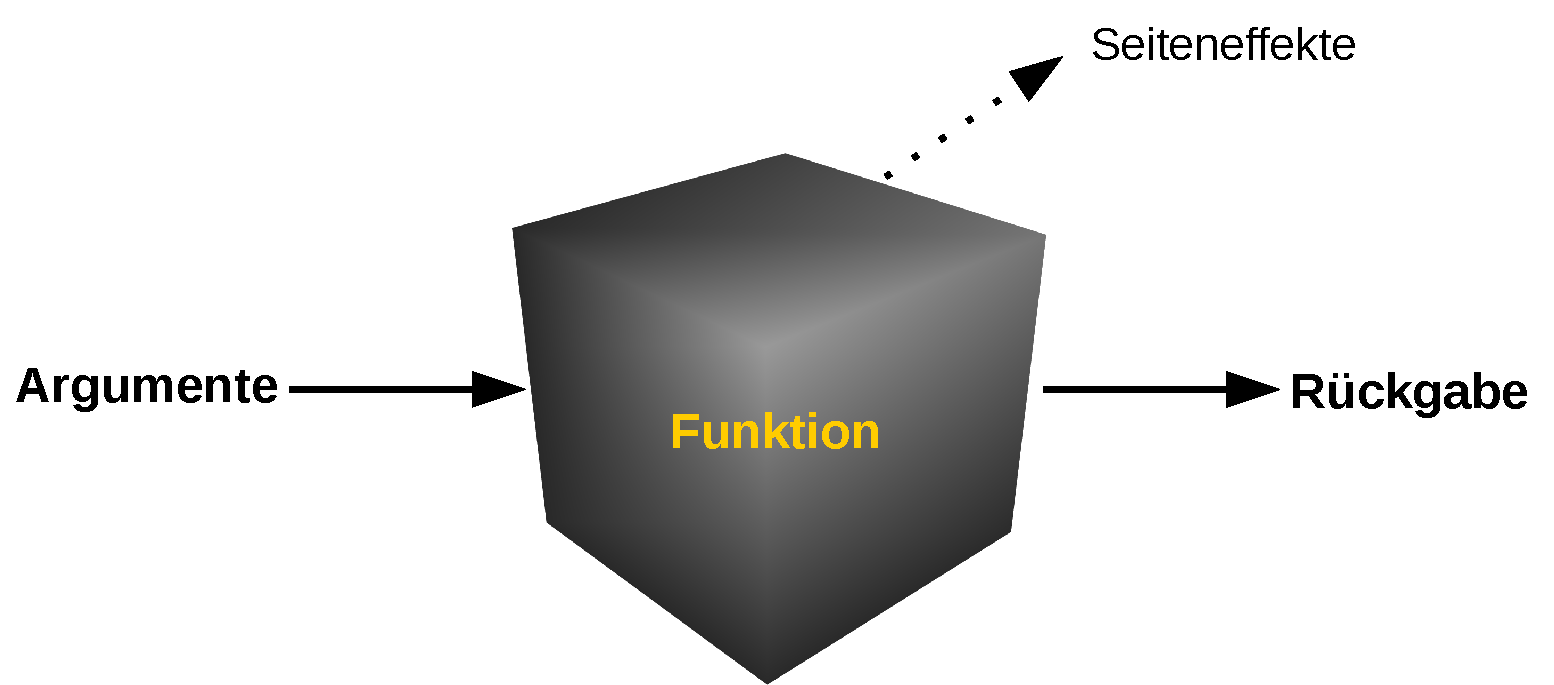
\includegraphics[]{../images/BlackBoxModel.pdf}
\end{center}

Funktionen nehmen Argumente an, die ihr Verhalten steuern. Sie geben
genau ein \texttt{R}-Objekt zurück, das Rückgabewert genannt wird. Wenn
der Aufruf einer Funktion außer dieser Rückgabe weitere Auswirkung auf
die ``Umgebung'' hat, nennt man das einen Seiteneffekt. Als
\texttt{R}-Neuling ist es manchmal wichtig einzusehen, was der
Unterschied zwischen den Seiteneffekten und der Rückgabe einer Funktion
ist.

Die innere Arbeitsweise von Funktionen wird als ``Black Box''
betrachtet. Wir wissen nicht unbedingt, wie eine Funktion intern
funktioniert, was uns aber auch nicht interessiert. So lange uns
\texttt{mean} den korrekten Mittelwert ausgibt, ist uns egal, wie
\texttt{mean} den Mittelwert berechnet.\footnote{Das ist natürlich
  zunächst einmal anders, wenn wir selbst neue Funktionen schreiben.
  Aber auch dann gilt: wenn ich die Funktion geschrieben habe und der
  Berechnung vertraue, kann ich später auf sie zugreifen, ohne mir jedes
  Mal über die interne Funktionsweise Gedanken zu machen. Das kann eine
  enorme Arbeitserleichterung sein.} Von Funktionen interessiert uns in
erster Linie, welche Daten wir einer Funktion als Argumente übergeben
müssen und was sie uns dafür in Austausch zurückgeben. Die folgenden
Abschnitte befassen sich mit den einzelnen Bestandteilen des
``Black-Box-Modells''.

\section{Argumente}\label{argumente}

Funktionsargumente determinieren das Verhalten von Funktionen. Im
einfachsten Fall bedeutet das, dass die Elemente eines Vektors, den wir
\texttt{mean} übergeben, den ausgegebenen Mittelwert determinieren. Wenn
wir gar keinen Vektor übergeben, erhalten wir kein Ergebnis, sondern
eine Fehlermeldung:

\begin{Shaded}
\begin{Highlighting}[]
\KeywordTok{mean}\NormalTok{()}
\NormalTok{Fehler }\ControlFlowTok{in} \KeywordTok{mean.default}\NormalTok{() }\OperatorTok{:}\StringTok{ }\NormalTok{Argument }\StringTok{"x"} \KeywordTok{fehlt}\NormalTok{ (ohne}
\NormalTok{Standardwert)}
\end{Highlighting}
\end{Shaded}

Um zu verstehen, wie man mit Argumenten das Verhalten von Funktionen
beeinflusst, ist ein Verständnis der folgenden Punkte wichtig:\footnote{Teilweise
  wurden diese Punkte schon in \protect\hyperlink{subset}{Kapitel 3 im
  Abschnitt zur Funktion \texttt{subset}} angesprochen.}

\begin{enumerate}
\def\labelenumi{\arabic{enumi}.}
\tightlist
\item
  Manche Argumente haben Standardwerte (Englisch: ``default values''),
  die angenommen werden, wenn wir diese Argumente beim Aufrufen der
  Funktion nicht explizit angeben. Diese Argumente heißen
  \emph{optionale Argumente}.
\item
  Wenn Argumente keinen Standardwert haben, \textbf{müssen} wir dem
  Argument einen Wert übergeben, da die Funktion sonst eine
  Fehlermeldung und kein Ergebnis ausgibt.
\item
  Argumente haben Namen, die wir verwenden können, um mit der Form
  ``\texttt{Argumentname\ =\ Wert}'' zu adressieren.
\item
  Wenn wir für ein Argument nicht explizit den Namen angeben, wird das
  Argument nach seiner Position in der Liste aller angegeben Argumente
  identifiziert.
\item
  Mit der \texttt{R}-Hilfe können wir herausfinden, welche Argumente
  Funktionen annehmen, wie diese heißen, und welche davon optional bzw.
  verpflichtend sind.
\end{enumerate}

Wir werden diese Punkte nun exemplarisch anhand der Funktion
\texttt{mean} nachvollziehen. Wir wissen bereits, dass \texttt{mean}
mindestens zwei Argumente annimmt. Beide Argumente haben Namen:

\begin{itemize}
\tightlist
\item
  \texttt{x}: der numerische oder logische Vektor, für den der
  Mittelwert bestimmt werden soll
\item
  \texttt{na.rm}: ein ein-elementiger logischer Vektor, der angibt, ob
  \texttt{NA}-Werte von der Berechnung ausgeschlossen werden sollen
\end{itemize}

Da der Aufruf \texttt{mean} ohne Angabe eines numerischen oder logischen
Vektors einen Fehler ergibt, ist uns klar, dass \texttt{x} kein
optionales Argument ist. Wir \textbf{müssen} einen Vektor übergeben, für
den wir einen Mittelwert bestimmen können. Sonst würde es auch keinen
Sinn machen, \texttt{mean} überhaupt aufzurufen.

Auf der anderen Seite wissen wir auch, dass wir das Argument
\texttt{na.rm} nicht unbedingt angeben müssen -- das würden wir
normalerweise nur dann machen, wenn wir wissen, dass unsere Daten
fehlende Werte enthalten. Folgender Aufruf funktioniert nämlich, ohne
dass wir dem Argument \texttt{na.rm} einen Wert übergeben:

\begin{Shaded}
\begin{Highlighting}[]
\KeywordTok{mean}\NormalTok{(}\DecValTok{1}\OperatorTok{:}\DecValTok{10}\NormalTok{)}
\end{Highlighting}
\end{Shaded}

\begin{verbatim}
[1] 5.5
\end{verbatim}

Doch was passiert mit \texttt{na.rm}, wenn wir es nicht explizit
angeben? Hierbei nehmen wir folgende Regel zur Kenntnis:
\textbf{optionale Argumente sind deswegen optional, da ihnen von der
Funktion ein Wert zugewiesen wird, wenn wir das Argument nicht selber
übergeben}. Das Argument \texttt{na.rm} hat den Standardwert
\texttt{FALSE}, weswegen \texttt{NA}-Werte im Normalfall nicht von der
Berechnung ausgeschlossen werden. Stattdessen wird uns \texttt{NA}
zurückgegeben, wenn \texttt{x} mindestens einen fehlenden Wert enthält.
Folgende Aufrufe sind demnach äquivalent:

\begin{Shaded}
\begin{Highlighting}[]

\KeywordTok{mean}\NormalTok{(}\DecValTok{1}\OperatorTok{:}\DecValTok{10}\NormalTok{)}
\KeywordTok{mean}\NormalTok{(}\DecValTok{1}\OperatorTok{:}\DecValTok{10}\NormalTok{, }\DataTypeTok{na.rm =} \OtherTok{FALSE}\NormalTok{)}
\end{Highlighting}
\end{Shaded}

Da wir nicht immer alle optionalen Argumente von Funktionen angeben
wollen -- stattdessen ``vertrauen'' wir auf die Standardwerte --, ist es
sehr hilfreich, dass wir Funktionsargumente per Namen ansprechen können.
So können wir nur genau die optionalen Argumente auswählen, die wir
anpassen wollen; für die anderen belassen wir den Standardwert. Das
haben wir bei der Funktion \texttt{mean} kennengelernt: nur wenn wir
fehlende Werte von der Berechnung des Mittelwerts ausschließen wollen,
weisen wir dem Argument \texttt{na.rm} den Wert \texttt{TRUE} zu:

\begin{Shaded}
\begin{Highlighting}[]
\KeywordTok{mean}\NormalTok{(}\KeywordTok{c}\NormalTok{(}\DecValTok{1}\NormalTok{, }\DecValTok{2}\NormalTok{, }\DecValTok{3}\NormalTok{, }\OtherTok{NA}\NormalTok{), }\DataTypeTok{na.rm =} \OtherTok{TRUE}\NormalTok{)}
\end{Highlighting}
\end{Shaded}

\begin{verbatim}
[1] 2
\end{verbatim}

Interessanterweise wissen wir bislang gar nicht, ob wir an dieser Stelle
\texttt{na.rm} tatsächlich mit Namen ansteuern müssen. In Funktionen
können wir Argumente ja anhand ihres Namens \emph{oder} ihrer Position
ansprechen. Wenn \texttt{na.rm} das zweite Argument wäre, könnten wir
auch folgenden Aufruf verwenden:

\begin{Shaded}
\begin{Highlighting}[]
\KeywordTok{mean}\NormalTok{(}\KeywordTok{c}\NormalTok{(}\DecValTok{1}\NormalTok{, }\DecValTok{2}\NormalTok{, }\DecValTok{3}\NormalTok{, }\OtherTok{NA}\NormalTok{), }\OtherTok{TRUE}\NormalTok{)}
\NormalTok{Fehler }\ControlFlowTok{in} \KeywordTok{mean.default}\NormalTok{(}\KeywordTok{c}\NormalTok{(}\DecValTok{1}\NormalTok{, }\DecValTok{2}\NormalTok{, }\DecValTok{3}\NormalTok{, }\OtherTok{NA}\NormalTok{), }\OtherTok{TRUE}\NormalTok{) }\OperatorTok{:}\StringTok{ }
\StringTok{  'trim'}\NormalTok{ must be numeric of length one}
\end{Highlighting}
\end{Shaded}

Das hat aber nicht funktioniert. Diese Fehlermeldung informiert uns
darüber, dass \texttt{mean} an der zweiten Position ein Argument mit dem
Namen ``\texttt{trim}'' erwartet. Offensichtlich hat \texttt{mean} mit
\texttt{trim} noch ein weiteres optionales Argument, das wir bislang gar
nicht kannten. Das heißt für uns: solange wir für \texttt{trim} -- was
auch immer das ist -- keinen Wert angeben, müssen wir \texttt{na.rm} per
Namen ansprechen.

Wenn wir Argumente mit Namen ansteuern, brauchen wir uns über die
Reihenfolge der Argumente keine Gedanken machen. Das ist oftmals sehr
hilfreich. Deswegen funktioniert folgender Aufruf:

\begin{Shaded}
\begin{Highlighting}[]
\KeywordTok{mean}\NormalTok{(}\DataTypeTok{na.rm =} \OtherTok{FALSE}\NormalTok{, }\DataTypeTok{x =} \DecValTok{1}\OperatorTok{:}\DecValTok{10}\NormalTok{)}
\end{Highlighting}
\end{Shaded}

\begin{verbatim}
[1] 5.5
\end{verbatim}

Unter Berücksichtigung unseres Wissens über die Vergabe von Namen bei
Funktionsargumenten erweitern wir nun das Beispiel von oben -- folgende
Aufrufe sind alle äquivalent:

\begin{Shaded}
\begin{Highlighting}[]
\KeywordTok{mean}\NormalTok{(}\DecValTok{1}\OperatorTok{:}\DecValTok{10}\NormalTok{)}
\KeywordTok{mean}\NormalTok{(}\DecValTok{1}\OperatorTok{:}\DecValTok{10}\NormalTok{, }\DataTypeTok{na.rm =} \OtherTok{FALSE}\NormalTok{)}
\KeywordTok{mean}\NormalTok{(}\DataTypeTok{x =} \DecValTok{1}\OperatorTok{:}\DecValTok{10}\NormalTok{)}
\KeywordTok{mean}\NormalTok{(}\DataTypeTok{x =} \DecValTok{1}\OperatorTok{:}\DecValTok{10}\NormalTok{, }\DataTypeTok{na.rm =} \OtherTok{FALSE}\NormalTok{)}
\KeywordTok{mean}\NormalTok{(}\DataTypeTok{na.rm =} \OtherTok{FALSE}\NormalTok{, }\DataTypeTok{x =} \DecValTok{1}\OperatorTok{:}\DecValTok{10}\NormalTok{)}
\end{Highlighting}
\end{Shaded}

Nicht äquivalent zu den obigen Aufrufen sind jedoch folgende Aufrufe,
die zu Fehlermeldungen führen, da \texttt{na.rm} nicht das zweite
Argument von \texttt{mean} ist:

\begin{Shaded}
\begin{Highlighting}[]
\KeywordTok{mean}\NormalTok{(}\DecValTok{1}\OperatorTok{:}\DecValTok{10}\NormalTok{, }\OtherTok{FALSE}\NormalTok{)}
\KeywordTok{mean}\NormalTok{(}\DataTypeTok{x =} \DecValTok{1}\OperatorTok{:}\DecValTok{10}\NormalTok{, }\OtherTok{FALSE}\NormalTok{)}
\end{Highlighting}
\end{Shaded}

Wir haben nun gelernt wie wir Argumente an Funktionen übergeben können.
Dieses Wissen hilft uns jedoch nur, wenn wir folgende Frage beantworten
können:

~

\textbf{Wie finden wir heraus, was für Argumente eine Funktion annimmt?}

\subsection{\texorpdfstring{Die
\texttt{R}-Hilfe}{Die R-Hilfe}}\label{help}

Wenn wir effektiv herausfinden können, wie wir \texttt{R}-Funktionen
bedienen -- welche Argumente wir ihnen also übergeben müssen -- sind wir
als \texttt{R} Nutzer in einer sehr komfortablen Position. Für sehr
viele statistische und testtheoretische Analysen wurden bereits
Funktionen geschrieben, die uns frei zugänglich sind. Wenn diese
Funktionen noch nicht in der Basisversion von \texttt{R} enthalten sind,
sind sie stattdessen häufig in externen Paketen verfügbar. So können wir
beispielsweise ANOVAs, explorative oder konfirmatorische
Faktorenanalysen und viele andere Auswertungen durchführen -- wenn wir
denn wollen. Wir benötigen dabei nur das folgende Wissen:

\begin{enumerate}
\def\labelenumi{\arabic{enumi}.}
\tightlist
\item
  Welche Funktion führt die gewünschte Berechnung aus?
\item
  Wie können wir diese Funktionen bedienen?
\end{enumerate}

Wir beschäftigen uns im Folgenden mit dem zweiten Punkt.\footnote{Auch
  wenn es häufig erst einmal der Knackpunkt ist zu wissen, ob es schon
  eine Funktion gibt, die das eigene Problem löst, wie diese heißt und
  in welchem Paket ich sie finde.} Wir lernen, wie wir uns mit der
\texttt{R}-Hilfe einen Überblick über die Arbeitsweise von Funktionen
verschaffen können. Probieren wir es exemplarisch für die Funktion
\texttt{mean} aus:

\begin{Shaded}
\begin{Highlighting}[]
\NormalTok{?mean}
\end{Highlighting}
\end{Shaded}

Interessant ist für erst einmal der obere Abschnitt ``Usage'':

\begin{Shaded}
\begin{Highlighting}[]
\NormalTok{Usage}\OperatorTok{:}

\StringTok{    }\KeywordTok{mean}\NormalTok{(x, ...)}

\NormalTok{    ## Default S3 method:}
    \KeywordTok{mean}\NormalTok{(x, }\DataTypeTok{trim =} \DecValTok{0}\NormalTok{, }\DataTypeTok{na.rm =} \OtherTok{FALSE}\NormalTok{, ...)}
\end{Highlighting}
\end{Shaded}

Wir ignorieren an dieser Stelle, dass uns zwei Varianten angeboten
werden, die Funktion \texttt{mean} zu nutzen.\footnote{Viele Funktionen
  können auf verschiedene Arten aufgerufen werden können. Das heißt: sie
  können mit unterschiedlichen \texttt{R}-Objekten als Eingabe genutzt
  werden.} Wenn in der Hilfe eine ``Default S3 method'' angeboten wird,
interessiert uns oftmals diese; so ist es auch hier der Fall. An dieser
Stelle finden wir die Informationen, die wir benötigen, um die Funktion
zu nutzen. Wir sehen

\begin{itemize}
\tightlist
\item
  die Namen der Argumente,
\item
  die Reihenfolge der Argumente,
\item
  welche Argumente optional sind,
\item
  was die Standardwerte der optionalen Argumente sind.
\end{itemize}

Die Standardwerte der optionalen Argumente lassen sich dadurch ablesen,
dass in der Argumentliste in der Form ``\texttt{Argumentname\ =\ Wert}''
schon ein Wert angegeben ist. Das Argument \texttt{trim} hat etwa den
Standardwert \texttt{0}. Wie wir bereits wissen, hat das Argument
\texttt{na.rm} hat den Standardwert \texttt{FALSE}. Bei nicht-optionalen
Argumenten ist kein Standardwert, sondern nur der Name des Arguments
angegeben.

Wenn wir mehr über die Argumente erfahren wollen, müssen wir den
Abschnitt ``Arguments'' der \texttt{R}-Hilfe konsultieren. Folgende
Punkte interessieren uns bei der Beschreibung:

\begin{enumerate}
\def\labelenumi{\arabic{enumi}.}
\tightlist
\item
  Was ist die inhaltliche Bedeutung eines Arguments
\item
  Was für ein \texttt{R}-Objekt muss ich übergeben, um ein Argument
  anzusteuern (z.B. Vektor; \texttt{data.frame}; \texttt{matrix};
  \texttt{list}; oder sogar eine Funktion -- siehe
  \protect\hyperlink{tapply}{Kapitel 3: Funktion tapply}).
\end{enumerate}

Die Beschreibung der Argumente achtet sehr auf Prägnanz und technische
Korrektheit, wie wir am Beispiel der Beschreibung der Argumente der
Funktion \texttt{mean} erkennen können:

\begin{verbatim}
Arguments:

    x: An R object.  Currently there are methods for 
       numeric/logical vectors and date, date-time and
       time interval objects. Complex vectors are allowed
       for ‘trim = 0’, only.

    trim: the fraction (0 to 0.5) of observations to
       be trimmed from each end of ‘x’ before the mean
       is computed.  Values of trim outside that range
       are taken as the nearest endpoint.

    na.rm: a logical value indicating whether ‘NA’ values
       should be stripped before the computation proceeds.
\end{verbatim}

Die \texttt{R}-Hilfe ist also hilfreich, aber nicht immer ganz leicht zu
nutzen. Oftmals ist eine weitere Google-Recherche oder das Nachfragen
bei einer Freundin oder einem Freund sinnvoll, wenn man die Nutzung
einer Funktion meistern will. Mehr Hilfe zur Nutzung einer Funktion
finden wir im Abschnitt ``Examples'' der \texttt{R}-Hilfe. Hier können
wir am konkreten Beispiel betrachten, wie die Funktion angewendet werden
kann. Wenn wir Glück haben, ist genau das dabei, was wir brauchen. Der
Code ist dabei so gewählt, dass man ihn \emph{Copy-\&-Paste} auch selber
in der Konsole ausführen kann. Bei \texttt{mean} finden wir etwa den
folgenden Beispiel-Code:

\begin{Shaded}
\begin{Highlighting}[]
\NormalTok{Examples}\OperatorTok{:}
\StringTok{     }\NormalTok{x <-}\StringTok{ }\KeywordTok{c}\NormalTok{(}\DecValTok{0}\OperatorTok{:}\DecValTok{10}\NormalTok{, }\DecValTok{50}\NormalTok{)}
\NormalTok{     xm <-}\StringTok{ }\KeywordTok{mean}\NormalTok{(x)}
     \KeywordTok{c}\NormalTok{(xm, }\KeywordTok{mean}\NormalTok{(x, }\DataTypeTok{trim =} \FloatTok{0.10}\NormalTok{))}
\end{Highlighting}
\end{Shaded}

\subsection{Namenlose Argumente}\label{namenlose-argumente}

In der Einführung in die Arbeitsweise von Funktionsargumenten habe ich
behauptet, dass Argumente Namen haben. Wie bei fast jeder allgemeinen
Regel, hat auch diese Regel Ausnahmen -- Argumente haben nämlich gar
nicht immer einen Namen. Das ist für uns zwar nicht ganz so wichtig,
aber wir können es hier zur Kenntnis nehmen. Wir haben sogar schon mit
Funktionen gearbeitet, die namenlose Argumente annehmen können. Das ist
beispielsweise immer dann notwendig, wenn Funktionen eine beliebige
Anzahl von Argumenten annehmen. Die Funktion \texttt{c} nimmt zum
Beispiel beliebig viele Vektoren entgegen, die dann zu einem Vektor
zusammengefügt werden. Auch andere Funktionen wie \texttt{table} -- die
beliebig viele Vektoren zur Erstellung von Kreuztabellen annimmt -- und
\texttt{dplyr::arrange} -- die beliebig viele Kriterien zur Sortierung
eines \texttt{data.frames} annimmt -- haben unbenannte Argumente. In der
\texttt{R}-Hilfe ist dies oftmals an dem Platzhalterargument
``\ldots{}'' (lies: \emph{ellipsis}) zu erkennen, siehe:\footnote{Wir
  nehmen interessiert zur Kenntnis, dass \texttt{c} zwei Argumente mit
  Standardwerten hat: \texttt{recursive} und \texttt{use.names}. Mit
  diesen Argumenten haben wir uns bislang nicht beschäftigt und das
  werden wir auch weiterhin nicht tun. Oftmals ``vertraut'' man den
  Standardwerten, wobei man damit früher oder später auch mal auf die
  Nase fallen wird.}

\begin{Shaded}
\begin{Highlighting}[]
\NormalTok{?c}

\NormalTok{Usage}\OperatorTok{:}

\StringTok{     }\NormalTok{## S3 Generic function}
\StringTok{     }\KeywordTok{c}\NormalTok{(...)}
     
\NormalTok{     ## Default S3 method:}
     \KeywordTok{c}\NormalTok{(..., }\DataTypeTok{recursive =} \OtherTok{FALSE}\NormalTok{, }\DataTypeTok{use.names =} \OtherTok{TRUE}\NormalTok{)}
     
\NormalTok{Arguments}\OperatorTok{:}

\StringTok{     }\NormalTok{...}\OperatorTok{:}\StringTok{ }\NormalTok{objects to be concatenated.}
\end{Highlighting}
\end{Shaded}

\section{Rückgabewerte}\label{ruxfcckgabewerte}

Der Rückgabewert einer Funktion ist das \texttt{R}-Objekt, das die
Funktion ausgibt. Jede Funktion hat einen Rückgabewert. Die Funktion
\texttt{mean} gibt beispielsweise einen ein-elementigen Vektor aus, der
das arithmetische Mittel des Eingabevektors repräsentiert. Die Funktion
\texttt{subset} gibt immer einen \texttt{data.frame} aus -- wie der
aussieht, bestimmen die Argumente, die wir der Funktion übergeben.

Das Verständnis von Rückgabewerten führt uns etwas tiefer in die
Innereien der \texttt{R}-Programmiersprache. Betrachten wir im folgenden
Beispiel die Funktion \texttt{t.test}, die einen \emph{t}-Test
durchführt und dabei die Mittelwerte zweier Vektoren vergleicht. Ich
verwende den NPI-Datensatz aus Kapitel 4 und vergleiche den mittleren
Narzissmus-Gesamtwert (Spalte \texttt{score}) zwischen weiblichen und
männlichen Testnehmenden (Spalte \texttt{gender}; Kodierung: männlich =
1, weiblich = 2).\footnote{An dieser Stelle ist es sinnvoll, noch einmal
  zu rekapitulieren, wie hier die Narzissmuswerte der Männer und Frauen
  ausgewählt werden.}

\begin{Shaded}
\begin{Highlighting}[]
\KeywordTok{t.test}\NormalTok{(npi}\OperatorTok{$}\NormalTok{score[npi}\OperatorTok{$}\NormalTok{gender }\OperatorTok{==}\StringTok{ }\DecValTok{1}\NormalTok{],}
\NormalTok{       npi}\OperatorTok{$}\NormalTok{score[npi}\OperatorTok{$}\NormalTok{gender }\OperatorTok{==}\StringTok{ }\DecValTok{2}\NormalTok{])}
\end{Highlighting}
\end{Shaded}

Wir erhalten folgende Ausgabe in der Konsole:

\begin{verbatim}

    Welch Two Sample t-test

data:  npi$score[npi$gender == 1] and npi$score[npi$gender == 2]
t = 13.249, df = 10681, p-value <
2.2e-16
alternative hypothesis: true difference in means is not equal to 0
95 percent confidence interval:
 1.801341 2.426906
sample estimates:
mean of x mean of y 
 14.19595  12.08183 
\end{verbatim}

Hier werden uns alle relevanten Aspekte der \emph{t}-Test-Berechnung
ausgegeben. Ein erster interessanter Hinweis ist, dass kein klassischer
\emph{t}-Test, sondern ein ``Welch Two Sample t-test'' gerechnet
wurde.\footnote{Setzt man das Argument \texttt{var.equal} auf
  \texttt{TRUE}, wird ein klassischer t-Test gerechnet (Standardwert:
  \texttt{FALSE}). Es ist etwas ironisch, dass die Funktion
  \texttt{t.test} keinen t-Test rechnet. Wenn man das erwartet, könnte
  man an dieser Stelle auf die Nase fallen, wenn man einfach auf die
  Standardwerte der Funktion vertraut. Mehr Informationen zum
  Welch-t-Test finden sich hier:
  \href{https://en.wikipedia.\%20org/wiki/\%20Welch\%27s_t-test}{https://en.wikipedia.org/wiki/Welch\%27s\_t-test}.}
Weiterhin werden uns t-Wert, Freiheitsgrade, p-Wert
(``\texttt{p-value\ \textless{}\ 2.2e-16}'' bedeutet: der p-Wert ist so
klein, dass vor dem ersten Wert hinter dem Komma, der \textbf{nicht}
Null ist, mindestens 16 Nullen stehen), das 95\%-Konfidenzintervall der
Differenz der mittleren Werte, sowie die Mittelwerte selbst ausgegeben.
Insgesamt kann man interpretieren, dass Männer im Mittel signifikant
höhere Narzissmuswerte aufweisen als Frauen. Aber dieser Befund ist für
uns in diesem Fall uninteressant -- wir wollen uns ja mit dem
Rückgabewert befassen. Was für ein \texttt{R}-Objekt wurde uns denn
ausgegeben?

Was in der Konsole angezeigt wird, stellt nicht direkt das
\texttt{R}-Objekt dar, das die Funktion \texttt{t.test} ausgibt. Es
handelt sich hierbei um eine etwas lesefreundlichere Zusammenfassung des
Tests. Um das tatsächlich ausgegebene Objekt zu inspizieren, kann ich
die Funktion \texttt{str} verwenden. Dazu speichere ich die Ausgabe des
t-Tests zunächst in einer Variablen ab:

\begin{Shaded}
\begin{Highlighting}[]
\NormalTok{test <-}\StringTok{ }\KeywordTok{t.test}\NormalTok{(npi}\OperatorTok{$}\NormalTok{score[npi}\OperatorTok{$}\NormalTok{gender }\OperatorTok{==}\StringTok{ }\DecValTok{1}\NormalTok{],}
\NormalTok{               npi}\OperatorTok{$}\NormalTok{score[npi}\OperatorTok{$}\NormalTok{gender }\OperatorTok{==}\StringTok{ }\DecValTok{2}\NormalTok{])}
\KeywordTok{str}\NormalTok{(test)}
\end{Highlighting}
\end{Shaded}

\begin{verbatim}
List of 9
 $ statistic  : Named num 13.2
  ..- attr(*, "names")= chr "t"
 $ parameter  : Named num 10681
  ..- attr(*, "names")= chr "df"
 $ p.value    : num 9.4e-40
 $ conf.int   : atomic [1:2] 1.8 2.43
  ..- attr(*, "conf.level")= num 0.95
 $ estimate   : Named num [1:2] 14.2 12.1
  ..- attr(*, "names")= chr [1:2] "mean of x" "mean of y"
 $ null.value : Named num 0
  ..- attr(*, "names")= chr "difference in means"
 $ alternative: chr "two.sided"
 $ method     : chr "Welch Two Sample t-test"
 $ data.name  : chr "npi$score[npi$gender == 1] and npi$score[npi$gender == 2]"
 - attr(*, "class")= chr "htest"
\end{verbatim}

Das von \texttt{t.test} ausgegebene Objekt ist eine ``List of 9'', also
eine Liste mit 9 Einträgen. Listen sind sehr allgemeine Datencontainer,
die Elemente von beliebigem Typ und beliebiger Zahl beinhalten
können.\footnote{Ein Eintrag einer Liste könnte beispielsweise eine
  andere Liste sein.} Listen stellen eine wichtige Datenstruktur in
\texttt{R} dar -- vielleicht ist es sogar die wichtigste Datenstruktur,
da \texttt{data.frames} spezielle Listen sind, in denen jeder Eintrag
(d.h., jede Spalte) ein Vektor gleicher Länge ist. Die Elemente der
Liste können benannt sein, wie es bei der Rückgabe von \texttt{t.test}
der Fall ist. In diesem Fall kann ich, wie wir es von der Spaltenauswahl
in \texttt{data.frames} kennen, mit der \texttt{\$}-Notation auf
einzelne Elemente zugreifen:

\begin{Shaded}
\begin{Highlighting}[]
\NormalTok{test}\OperatorTok{$}\NormalTok{statistic  }\CommentTok{# t-Wert als ein-elementiger Vektor}
\end{Highlighting}
\end{Shaded}

\begin{verbatim}
       t 
13.24906 
\end{verbatim}

\begin{Shaded}
\begin{Highlighting}[]
\NormalTok{test}\OperatorTok{$}\NormalTok{alternative  }\CommentTok{# ein- oder zweiseitiger Test?}
\end{Highlighting}
\end{Shaded}

\begin{verbatim}
[1] "two.sided"
\end{verbatim}

\begin{Shaded}
\begin{Highlighting}[]
\NormalTok{test}\OperatorTok{$}\NormalTok{parameter  }\CommentTok{# Freiheitsgrade}
\end{Highlighting}
\end{Shaded}

\begin{verbatim}
     df 
10681.4 
\end{verbatim}

Es ist nicht unüblich, dass komplexere statistische Berechnungen eine
Liste als Ausgabeobjekt ergeben. Listen sind dann sinnvoll, wenn während
der Berechnung mehrere Werte anfallen und es nützlich ist, diese an den
Nutzer zurückzugeben. Im Falle des t-Tests interessieren uns etwa die
Freiheitsgrade, der t-Wert und der p-Wert.

\section{Seiteneffekte}\label{seiteneffekte}

Jede Funktion hat genau einen Rückgabewert, also genau ein
\texttt{R}-Objekt, das von der Funktion zurückgegeben wird. Jegliche
Auswirkungen, die eine Funktion darüber hinaus hat -- außerhalb der
inneren Arbeitsweise --, werden Seiteneffekte genannt. Beispielsweise
war die Konsolen-Ausgabe der Funktion \texttt{t.test} im oberen Fall ein
Seiteneffekt. Wenn ich die Funktion \texttt{t.test} aufrufe, wird mir
eine Zusammenfassung des Tests in der Konsole ausgeben, die als Mensch
etwas einfacher zu verarbeiten ist als die Liste, die die
``tatsächliche'' Rückgabe darstellt. Das Zeichnen von Abbildungen ist
auch als Seiteneffekt zu verstehen. Wenn wir beispielsweise
\texttt{hist(npi\$score)} aufrufen, wird uns ein Histogramm der
Narzissmuswerte des NPI angezeigt. Dieses Histogramm ist ein
Seiteneffekt und nicht die Ausgabe der Funktion \texttt{hist};
Interessierte sind aufgefordert herausfinden, was deren tatsächliche
Rückgabe ist.

Ich werde die Diskussion von Seiteneffekten bei dieser kurzen und
oberflächlichen Einführung belassen. Manchmal ist die Unterscheidung in
Seiteneffekte und Rückgabe sinnvoll; wenn wir etwa die Ergebnisse einer
Funktion weiter verwenden möchten, ist es wichtig zu wissen, welche
Datenstruktur die Funktion ausgibt und wie wir auf die ausgegebenen
Werte zugreifen können. Um Power-Analysen für t-Tests zu simulieren
(eine Einführung in solche Simulationen wird in Kapitel 7 folgen), ist
es beispielsweise nötig, die exakten p-Werte aus der Ausgabe der
Funktion \texttt{t.test} auszulesen. In dem Fall werden wir die Funktion
\texttt{t.test} gegebenenfalls 10,000 Mal aufrufen und können es uns
nicht leisten, den p-Wert jedes Mal aus der Konsolen-Ausgabe abzulesen.
Stattdessen wollen wir den Prozess der p-Wert-Extraktion automatisieren;
und genau für solche Automatisierungen lernen wir das Programmieren.

\section{Selbst geschriebene
Funktionen}\label{selbst-geschriebene-funktionen}

Das Schreiben eigener Funktionen sollte früher oder später zum
Repertoire eines \texttt{R}-Nutzers gehören. Mit selbst geschriebenen
Funktionen können wir häufig durchgeführte Berechnungen abstrahieren und
beliebig oft durchführen. Betrachten wir den folgenden Code:

\begin{Shaded}
\begin{Highlighting}[]
\NormalTok{(}\FloatTok{0.23} \OperatorTok{*}\StringTok{ }\DecValTok{2}\NormalTok{)}\OperatorTok{/}\NormalTok{(}\DecValTok{1} \OperatorTok{+}\StringTok{ }\NormalTok{(}\DecValTok{2} \OperatorTok{-}\StringTok{ }\DecValTok{1}\NormalTok{) }\OperatorTok{*}\StringTok{ }\FloatTok{0.23}\NormalTok{)}
\NormalTok{(}\FloatTok{0.47} \OperatorTok{*}\StringTok{ }\DecValTok{3}\NormalTok{)}\OperatorTok{/}\NormalTok{(}\DecValTok{1} \OperatorTok{+}\StringTok{ }\NormalTok{(}\DecValTok{3} \OperatorTok{-}\StringTok{ }\DecValTok{1}\NormalTok{) }\OperatorTok{*}\StringTok{ }\FloatTok{0.23}\NormalTok{)  }\CommentTok{# copy-paste Fehler}
\NormalTok{(}\FloatTok{0.68} \OperatorTok{*}\StringTok{ }\DecValTok{4}\NormalTok{)}\OperatorTok{/}\NormalTok{(}\DecValTok{1} \OperatorTok{+}\StringTok{ }\NormalTok{(}\DecValTok{4} \OperatorTok{-}\StringTok{ }\DecValTok{1}\NormalTok{) }\OperatorTok{*}\StringTok{ }\FloatTok{0.68}\NormalTok{)}
\end{Highlighting}
\end{Shaded}

Erkennt ihr, was berechnet wird? Falls nicht, betrachtet diesen Code:

\begin{Shaded}
\begin{Highlighting}[]
\KeywordTok{spearman_brown}\NormalTok{(}\FloatTok{0.23}\NormalTok{, }\DecValTok{2}\NormalTok{)}
\KeywordTok{spearman_brown}\NormalTok{(}\FloatTok{0.37}\NormalTok{, }\DecValTok{3}\NormalTok{)}
\KeywordTok{spearman_brown}\NormalTok{(}\FloatTok{0.68}\NormalTok{, }\DecValTok{4}\NormalTok{)}
\end{Highlighting}
\end{Shaded}

In der ersten Variante sind nur ein paar Zahlen und arithmetische
Operationen zu sehen, die Semantik der Berechnung ist jedoch vollkommen
unklar. Durch das copy-pasten des Codes ist mir sogar ein Fehler
unterlaufen, denn ich habe in der zweiten Zeile einmal vergessen den
Wert 0.23 durch 0.47 auszutauschen -- solche Fehler passieren häufig und
sind sehr schwierig zu entdecken \citep[siehe][]{li2006}. Durch die
Nutzung der Funktion, die ich in Kapitel 4 definiert habe, ist der Code
lesbarer geworden und einfach interpretierbar: ich möchte drei
Reliabilitätsschätzer um die Faktoren 2, 3 bzw. 4 korrigieren. Sofern
ich bei der Definition meiner Funktion keinen Fehler gemacht habe, sind
diese Aufrufe auch robuster gegenüber Copy-Paste-Fehlern.

Mit eigenen Funktionen folgen wir dem Programmierer-Credo „\emph{do not
repeat yourself}``. Wenn wir einmal Code zur Lösung eines Problems
geschrieben haben, möchten wir denselben Code nicht noch einmal
schreiben, um ein gleiches bzw. ähnliches Problem zu lösen. Eigene
Funktionen helfen uns effizienter -- man könnte sogar sagen: fauler --
zu arbeiten. Außerdem führen sie zu besser lesbarem Code, denn
Funktionsnamen\footnote{Wie bei Variablen ist auch bei Funktionen eine
  sinnvolle Benennung unerlässlich.} kommunizieren die Intention von
Code deutlich besser als das reine Aneinanderreihen von Zahlen,
Operatoren und Variablen.

\subsection{Definition der eigenen
Funktion}\label{definition-der-eigenen-funktion}

Erinnern wir uns an die Spearman-Brown-Funktion, die ich in Kapitel 4
definiert habe:

\begin{Shaded}
\begin{Highlighting}[]
\DecValTok{1}\NormalTok{   spearman_brown <-}\StringTok{ }\ControlFlowTok{function}\NormalTok{(reliability, factor) \{}
\DecValTok{2}\NormalTok{       numerator  <-}\StringTok{ }\NormalTok{reliability }\OperatorTok{*}\StringTok{ }\NormalTok{factor}
\DecValTok{3}\NormalTok{       denominator <-}\StringTok{ }\DecValTok{1} \OperatorTok{+}\StringTok{ }\NormalTok{(factor}\DecValTok{-1}\NormalTok{) }\OperatorTok{*}\StringTok{ }\NormalTok{reliability}
\DecValTok{4}\NormalTok{       corrected_reliability <-}\StringTok{ }\NormalTok{numerator }\OperatorTok{/}\StringTok{ }\NormalTok{denominator}
\DecValTok{5}       \KeywordTok{return}\NormalTok{(corrected_reliability)}
\DecValTok{6}\NormalTok{   \}}
\end{Highlighting}
\end{Shaded}

Um die Funktion zu definieren, führe ich diese sechs Zeilen Code einfach
in der \texttt{R}-Konsole aus. In RStudio reicht es sogar, STRG-Enter zu
drücken, wenn sich mein Cursor in Zeile 1 befindet. In dieser Zeile
beginnt die Definition der Funktion: ich erstelle eine Variable, der ich
mit ``\texttt{\textless{}-}'' eine Funktion zuweise. Die Funktion
\texttt{spearman\_brown} wird also mit der Funktion \texttt{function}
erstellt (kein Witz). Die Funktion \texttt{function} nimmt die Argumente
entgegen, die auch meine neu definierte Funktion
\texttt{spearman\_brown} annehmen soll. Die Parameter, die bei der
Spearman-Brown-Korrektur eine Rolle spielen, sind der
Reliabilitätsschätzer und der Korrekturfaktor. Aus diesem Grund werden
die zwei Argumente \texttt{reliability} und \texttt{factor} definiert.

Auf die Definition der Argumente folgt der ``Körper'' (engl.:
\emph{body}) der Funktion. Der Körper führt die gewünschte Berechnung
durch und verwendet dabei die Funktionsargumente als Variablen.
Funktionsargumente sind also nichts anderes als Variablen, die im Innern
einer Funktion leben. Der Körper der Funktion wird in geschwungenen
Klammern \texttt{\{·\}} eingeschlossen. Solche Klammern bilden einen
abgeschlossenen Block von \texttt{R}-Code; sie werden uns auch im
nächsten Kapitel bei der Verwendung von Schleifen wieder begegnen.

In Zeile 5 wird mit der Funktion \texttt{return}\footnote{Es ist nicht
  unbedingt nötig, \texttt{return} zur Definition von Rückgabewerten zu
  verwenden. Aber ich mache es immer so und verrate die Alternative auch
  nicht.} angegeben, dass die Variable \texttt{corrected\_reliability}
von der Funktion zurückgegeben werden soll. Das heißt: das
\texttt{R}-Objekt, das innerhalb der Funktion in die Variable
\texttt{corrected\_reliability} geschrieben wird, ist der Rückgabewert
der Funktion.

\subsection{Lokale Variablen}\label{lokale-variablen}

Werfen wir noch einmal einen Blick auf den Körper der Funktion
\texttt{spearman\_brown}. Wir sehen hier bereits gewohnten
\texttt{R}-Code -- nichts besonderes: Variablen werden geschrieben und
Berechnungen werden durchgeführt. Ein wichtiger Punkt an diesen
Berechnungen ist jedoch, dass sie nur innerhalb der Funktion stattfinden
und keine Wirkungen ``nach außen'' haben. Was heißt das konkret?
Beispielsweise sind alle Variablen, die innerhalb der Funktion definiert
werden, sogenannte \emph{lokale} Variablen. Das heißt: sie sind
außerhalb der Funktion nicht sichtbar und verschwinden nach Aufruf der
Funktion wieder. Es ist also nicht so, dass bei Aufruf der Funktion die
Variablen \texttt{numerator}, \texttt{denominator} und
\texttt{corrected\_reliability} in die \texttt{R}-Umgebung geschrieben
werden.\footnote{Dies ist ein weiterer Vorteil der Verwendung von
  Funktionen. Viele Variablen, die ich schreibe, brauche ich nicht
  unbedingt in meiner Umgebung; sie sind nur Mittel zum Zweck. Durch die
  Verwendung von Funktionen bleiben solche Hilfsvariablen verdeckt.} Nur
der Rückgabewert dringt nach außen; ich kann ihn abfangen, indem ich ihn
in einer Variablen abspeichere, etwa wie folgt:

\begin{Shaded}
\begin{Highlighting}[]
\NormalTok{split_half_correct <-}\StringTok{ }\KeywordTok{spearman_brown}\NormalTok{(}\FloatTok{0.63}\NormalTok{, }\DecValTok{2}\NormalTok{)}
\end{Highlighting}
\end{Shaded}

Durch diesen Befehl wird eine korrigierte Reliabilität in eine Variable
mit dem Namen \texttt{split\_half\_correct} geschrieben; dass der
Rückgabewert der Funktion innerhalb der Funktion in einer Variablen mit
dem Namen \texttt{corrected\_reliability} abgespeichert ist, ist für das
ausgegebene Objekt nicht von Bedeutung.

Argumente sind ebenfalls lokale Variablen in der Funktion. Wenn wir
einer Funktion also ein Argument übergeben, definieren wir damit eine
lokale Variable mit dem Namen des Arguments innerhalb der Funktion.
Daraus können wir beispielsweise schließen, dass im Code der Funktion
\texttt{mean} irgendwo eine Variable mit dem Namen \texttt{na.rm}
verwendet wird.

\subsection{Optionale Argumente}\label{optionale-argumente}

Bei der Definition einer Funktion können wir Standardwerte vergeben und
somit optionale Argumente definieren. Wenn wir beispielsweise davon
ausgehen, dass wir die Spearman-Brown-Korrektur meistens verwenden, um
eine Split-Half-Korrelation zu korrigieren, könnten wir das Argument
\texttt{factor} per default wie folgt auf 2 setzen:

\begin{Shaded}
\begin{Highlighting}[]
\NormalTok{spearman_brown <-}\StringTok{ }\ControlFlowTok{function}\NormalTok{(reliability, }\DataTypeTok{factor =} \DecValTok{2}\NormalTok{) \{}
\NormalTok{    ...}
\NormalTok{\}}
\end{Highlighting}
\end{Shaded}

Diese Schreibweise kennen wir schon vom Aufruf von Funktionen, wenn wir
die Argumente mit Namen ansprechen. In diesem Fall können wir die
Funktion \texttt{spearman\_brown} auch wie folgt äquivalent verwenden:

\begin{Shaded}
\begin{Highlighting}[]
\NormalTok{split_half_correct <-}\StringTok{ }\KeywordTok{spearman_brown}\NormalTok{(}\FloatTok{0.63}\NormalTok{)}
\NormalTok{split_half_correct <-}\StringTok{ }\KeywordTok{spearman_brown}\NormalTok{(}\FloatTok{0.63}\NormalTok{, }\DecValTok{2}\NormalTok{)}
\end{Highlighting}
\end{Shaded}

\subsection{Wann schreibe ich meine eigene
Funktion}\label{wann-schreibe-ich-meine-eigene-funktion}

Wie wir in den letzten Abschnitten gesehen haben, ist die technische
Definition einer Funktion keine schwierige Sache. Schwieriger ist
häufiger die Antwort auf die Frage, wann ich tatsächlich eine Funktion
schreiben will. Darauf gibt es keine einzige richtige Antwort, und am
Ende muss jeder für sich selbst entscheiden. Generell ist eine sinnvolle
Daumenregel, dann eine Funktion zu schreiben, wenn man denselben Code
mehrfach geschrieben hat. Häufiges \emph{copy-\&-pasten} kann da ein
guter Indikator sein. In dem Fall solltet ihr identifizieren, welche
Details sich jeweils bei den verschiedenen Varianten des Codes geändert
haben, und diese in Argumente umwandeln.

Um zu erkennen, wann Funktionen nützlich sind und welche Variablen man
als Argumente umsetzen will, bedarf es sicherlich einiger Erfahrung mit
\texttt{R}. Mein Tipp für Anfänger ist deswegen vor allem: erst mal
einfach ``coden'' -- später Funktionen schreiben. Mit mehr Erfahrung
kann sich diese Vorgehensweise ändern. Ich überlege oftmals schon in der
Planungsphase eines Projekts, welche Funktionen sich sinnvollerweise
anbieten und wie diese zusammen arbeiten sollten. Aber das Vorgehen
hängt auch stark von der Art des Projekts ab. Wenn ich bloß Daten
einlese und einen t-Test oder eine ANOVA rechne, muss ich dafür keine
Funktion schreiben. Wenn ich hingegen viel mit Daten an sich arbeite --
also oft Daten auswähle, transformiere, etc. --, machen eigene
Funktionen oftmals mehr Sinn.

\section{Fragen zum vertiefenden
Verständnis}\label{fragen-zum-vertiefenden-verstuxe4ndnis-3}

\begin{enumerate}
\def\labelenumi{\arabic{enumi}.}
\tightlist
\item
  Was ist der Rückgabewert der Funktion \texttt{str}?
\item
  Was ist der Rückgabewert der Funktion \texttt{hist}?
\item
  Kann ich mit der Funktion \texttt{spearman\_brown} gleichzeitig
  mehrere Reliabilitätsschätzer korrigieren? (Code inspizieren \(\to\)
  überlegen \(\to\) ausprobieren)
\end{enumerate}

\chapter{Schleifen}\label{schleifen}

Inhalt folgt.

\chapter{Simulationen}\label{simulationen}

Inhalt folgt.

\chapter{Anhang}\label{anhang}

Dieser Abschnitt arbeitet einige Schwierigkeiten auf, die sich in den
praktischen Übungen des Seminars ergeben haben.

\hypertarget{datenEinlesen}{\section{Daten
einlesen}\label{datenEinlesen}}

Das Einlesen von Daten in \texttt{R} stellt uns vor verschiedene
Probleme. Ich gehe an dieser Stelle auf ein grundlegendes Problem ein,
das sich bei dem Einlesen jeglicher Daten stellt (egal ob man SPSS,
Excel, csv, oder sonstige Dateien einliest): Woher weiß \texttt{R}, wo
sich die Daten befinden, die ich einlesen möchte? Die Festplatte ist
groß -- \texttt{R} kann nur wissen, in welchem Ordner Daten liegen, wenn
wir es \texttt{R} verraten.

Unsere Strategie: Wir verwenden RStudio-Projekte. Beachtet, dass dies
nur eine von verschiedenen Möglichkeiten ist, mit dem
``Dateisuchproblem'' umzugehen. Aber es ist eben die, die wir nutzen.
\textbf{Beachtet ebenfalls, dass das das Einzige ist, wofür wir RStudio
Projekte nutzen: Wir legen RStudio Projekte an, um \texttt{R}
mitzuteilen, wo es nach Daten suchen soll.} Bevor wir ein RStudio
Projekt anlegen, müssen wir wissen, wo auf unserem Computer der
Datensatz liegt. Wenn wir das wissen, legen wir in dem entsprechenden
Ordner wie folgt ein Projekt an:

~

\(\to\) File\\
\(\to\) New project\\
\(\to\) Associate a project with an existing working directory\\
\(\to\) Browse\\
\(\to\) \emph{Zum Ordner navigieren}\\
\(\to\) Open\\
\(\to\) Create Project

~

Nach dem Anlegen startet sich RStudio neu und unten rechts im Panel wird
der Inhalt des Projekt-Ordners angezeigt. Wenn wir das Projekt gestartet
haben, können wir Daten einlesen, die in diesem Ordner liegen. Dafür
werden wir Funktionen aufrufen, die den Datensatz mit Dateinamen
ansteuern. Folgender Aufruf etwa könnte eine csv-Datei einlesen und die
Tabelle als \texttt{data.frame} in der Variablen \texttt{tp} speichern.

\begin{Shaded}
\begin{Highlighting}[]
\NormalTok{tp <-}\StringTok{ }\KeywordTok{read.csv}\NormalTok{(}\StringTok{"technophobie.csv"}\NormalTok{)}
\end{Highlighting}
\end{Shaded}

Wenn wir schon einmal ein Projekt im Ordner mit unseren Daten angelegt
haben, können wir das Projekt beim nächsten Mal wieder aufrufen. Dafür
gehen wir über

~

\(\to\) Open Project\\
\(\to\) \emph{Zum Ordner navigieren}\\
\(\to\) \emph{Projektdatei auswählen} (hat die Endung .Rproj) \(\to\)
\emph{Öffnen}

\section{Das Environment sauber
halten}\label{das-environment-sauber-halten}

Wenn wir in \texttt{R} arbeiten, ist es wichtig, dass wir einen
Überblick über die Variablen haben, die gerade existieren. Im Folgenden
beschreibe ich ein paar grundlegende Strategien, um unsere
\texttt{R}-Arbeitsumgebung einigermaßen sauber zu halten.

\subsection{Variablen löschen}\label{variablen-luxf6schen}

RStudio gibt uns in einem Panel oben rechts darüber Auskunft, welche
Variablen sich in unserem sogenannten \emph{Environment} befinden. Darin
kommen alle Variablen vor, die wir irgendwann mit einer Zuweisung
(``\texttt{\textless{}-}'') erstellt haben. Um ein bisschen Ordnung zu
halten, ist es nützlich zu wissen, wie man einzelne oder alle Variablen
wieder entfernen kann. Es kann schnell passieren, dass man sehr viele
Variablen erstellt, über die man sonst die Übersicht verliert.

Mit der Funktion \texttt{rm} kann man Variablen löschen, etwa:

\begin{Shaded}
\begin{Highlighting}[]
\NormalTok{foo <-}\StringTok{ }\DecValTok{1}\OperatorTok{:}\DecValTok{10}
\KeywordTok{rm}\NormalTok{(foo)}
\end{Highlighting}
\end{Shaded}

Möchte man alle Variablen aus dem Environment löschen, kann man den
Befehl \texttt{rm(list\ =\ ls())} verwenden, etwa:

\begin{Shaded}
\begin{Highlighting}[]
\NormalTok{foo <-}\StringTok{ }\DecValTok{1}\OperatorTok{:}\DecValTok{10}
\NormalTok{bar <-}\StringTok{ }\DecValTok{1}\OperatorTok{:}\DecValTok{100}
\NormalTok{gaz <-}\StringTok{ }\KeywordTok{mean}\NormalTok{(bar)}
\KeywordTok{rm}\NormalTok{(}\DataTypeTok{list =} \KeywordTok{ls}\NormalTok{()) }\CommentTok{# löscht alles, nur mit Vorsicht verwenden}
\end{Highlighting}
\end{Shaded}

\subsection{Mit einem sauberen Environment
starten}\label{mit-einem-sauberen-environment-starten}

Wenn man RStudio beendet, wird einem von RStudio die Frage gestellt, ob
man seinen ``workspace'' abspeichern will. Das kann etwa so aussehen,
bei euch sieht es gegebenenfalls ein wenig anders aus:

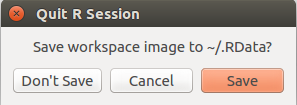
\includegraphics{../images/SaveWorkspace.png}

Wenn man in diesem Fall zustimmt, wird im derzeitigen ``working
directory'' -- für uns heißt das: der Ordner unseres RStudio Projekts --
eine Datei mit dem Namen ``.RData'' abgelegt. Diese Datei enthält alle
Variablen, die sich derzeit in unserem Environment befinden. Also alle
Variablen, die uns oben rechts im Panel auch angezeigt werden. Wenn wir
zustimmen und das Projekt aus dem Ordner neu laden, werden beim nächsten
Mal alle Variablen unserer Session neu geladen. Ich rate stark davon ab,
so zu arbeiten. Ich würde bevorzugen, \textbf{immer}\footnote{Natürlich
  gibt es auch hier Ausnahmen. Wenn ihr selber einen Grund findet, aus
  dem es für euch doch gut ist, die Variablen abzuspeichern -- etwa weil
  das Dateneinlesen sonst sehr lange dauert --, dann macht bitte das,
  was für euch sinnvoll ist.} mit einem leeren Environment zu starten.
Der einfachste Weg, um dies zu bewerkstelligen, ist immer ``Don't save''
auszuwählen, wenn man gefragt wird. Wenn man aus Versehen mal auf
``Save'' geklickt hat, kann man das Environment beim nächsten Start des
Projekts mit dem Befehl \texttt{rm(list\ =\ ls())} wieder leeren. Auf
Dauer hilft dann aber nur, die angelegte Datei im RStudio Projektordner
zu löschen (diese wird vermutlich ``.RData'' heißen).

\bibliography{referenzen.bib}



\end{document}
